\scanpage{1}
\figure{%
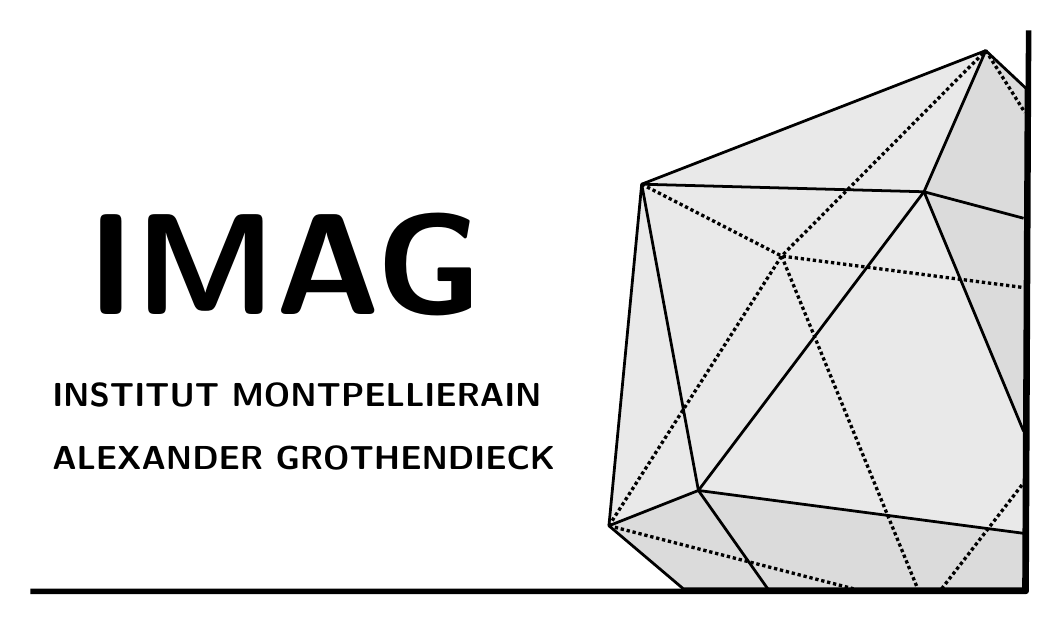
\begin{tikzpicture}[x=0.016cm,y=-0.016cm,line join=round]
\node[anchor=west,font=\sffamily\bfseries,scale=5.2] at (17,202) {IMAG};
\node[anchor=west,font=\sffamily\bfseries,scale=1.2] at (20,305) {INSTITUT MONTPELLIERAIN};
\node[anchor=west,font=\sffamily\bfseries,scale=1.2] at (20,355) {ALEXANDER GROTHENDIECK};
\path[fill=gray!17] (497,138)--(770,32)--(802,62)--(800,459)--(530,459)--(471,409)--cycle;
\path[fill=gray!28] (770,32)--(802,62)--(800,334)--(721,144)--cycle;
\path[fill=gray!28] (471,409)--(542,381)--(800,415)--(800,459)--(530,459)--cycle;
\draw[line width=1pt] (497,138)--(770,32)--(802,62)--(800,459)--(530,459)--(471,409)--cycle;
\draw[line width=1pt] (497,138)--(721,144)--(800,165);
\draw[line width=1pt] (770,32)--(721,144)--(542,381)--(471,409);
\draw[line width=1pt] (497,138)--(542,381)--(597,459);
\draw[line width=1pt] (542,381)--(800,415);
\draw[line width=1pt] (721,144)--(800,334);
\draw[densely dotted,line width=1.2pt] (497,138)--(608,195)--(800,220);
\draw[densely dotted,line width=1.2pt] (471,409)--(608,195)--(770,32);
\draw[densely dotted,line width=1.2pt] (608,195)--(716,459);
\draw[densely dotted,line width=1.2pt] (471,409)--(665,459);
\draw[densely dotted,line width=1.2pt] (735,459)--(800,375);
\draw[densely dotted,line width=1.2pt] (770,32)--(801,81);
\draw[line width=2pt] (12,461)--(802,461)--(804,16);
\end{tikzpicture}}

\scanpage{2}
\margin{(\unsure{10 p})}
\uline{Calculs des} $S_0\unsure{\mathcal{T}}_G$
\mspage{1}

\scanpage{3}
\mspage{I}
\uline{Calcul de} $S_0\mathcal{T}_G$, \uline{pour} $G$ \uline{\unsure{graphe}} MD \uline{de dim. modulaire} $0$.

\margin{\unsure{On notera} plutôt $S_0^{\circ}\mathcal{T}_G$ \unsure{pour ces} groupoïdes \unsure{étriqués|extrêmes}, \unsure{car} \unsure{bien trop petits}\unsure{]|)}}

$S_0\mathcal{T}_G$ est un $\mathbb{Z}^{\widehat{A}}$-groupoïde, déduit du $\mathbb{Z}^{\widehat{\vec A}}$-groupoïde $S_0\mathcal{T}_{G^b}$ par le changement de groupe \deleted{\unsure{en}} \unsure{interne}
\[
\mathbb{Z}^{\widehat{\vec A}}\longrightarrow\mathbb{Z}^{\widehat A}
\qquad\text{associé à}\qquad
\widehat{\vec A}\longrightarrow\widehat A
\]
i.e.
\[
(1)\qquad S_0\mathcal{T}_G=S_0\mathcal{T}_{G^b}\wedge_{\mathbb{Z}^{\widehat{\vec A}}}\mathbb{Z}^{\widehat A}
\]
et
\[
(2)\qquad S_0\mathcal{T}_{G^b}=\prod_{s\in S}S_0\mathcal{T}_{G_s^b}
=\prod_{s\in S}S_0\mathcal{T}_{0,\widehat{\vec A}_s}
\]
ce qui nous \unsure{ramène} à décrire $S_0\mathcal{T}_G$, quand $G$ est un \unsure{démigraphe} ayant un seul sommet, donc can$^{\mathrm t}$. isomorphe à un $G_{0,I}$, $I$ étant un ens. à trois éléments, \deleted{de sorte} -- i.e. on est ramené à décrire \deleted{\illegible{1}} $S_0\mathcal{T}_{0,I}$.

Considérons \unsure{la} \deleted{courbe}\inserted{droite} projective $I$-marquée sur $\mathbb C$, $\mathbb P^1_I$. Soit $\omega(I)$ l'ens des deux orientations de $I$. Si $\alpha\in\omega(I)$, on a des iso. canoniques \inserted{de $\mathbb U$-torseurs} pour les espaces tangents unitaires $T_i$ \unsure{en les} $i\in I\subset\mathbb P^1_I$
\[
T_i\overset{\varphi_{\alpha,i}}{\underset{\sim}{\longleftrightarrow}}\mathbb U
=\{z\in\mathbb C\mid |z|=1\}
\]
i.e. un isom de $\mathbb U^I$-torseurs
\[
\mathbb U^I\xrightarrow[\sim]{\varphi}P\mathbb U_G=P\mathbb U_{0,I}=\prod_{i\in I}T_i
\]
i.e. un point \deleted{noté} $\bar\alpha=\varphi(1)\in P\mathbb U_{0,I}$, d'où un plongement canonique
\[
(3)\qquad\omega(I)\hookrightarrow P\mathbb U_{0,I}
\]
compatible avec l'homomorphisme sur les groupes d'opérateurs

$(4)$\quad
\diagram{\begin{tikzcd}[ampersand replacement=\&, column sep=large,row sep=large]
\{\pm1\}\arrow[rr]\arrow[dr,"\mathrm{diag}"']\&\&\mathbb U^I\\
\&\{\pm1\}^I\arrow[ur,"{\substack{\text{déduit de l'inclusion}\\\{\pm1\}\hookrightarrow\mathbb U}}"']\&
\end{tikzcd}}
\mspage{2}

\scanpage{4}
Bien entendu, (3) et (4) sont compatibles avec l'action de $\unsure{\mathfrak S}_I$ (qui opère sur $\omega(I)$ par la signature).

Je définis $S_0\mathcal T_{0,I}$ comme le \unsure{ss-groupoïde} du groupoïde fondamental de $P\mathbb U_{0,I}$ induit \deleted{\unsure{par}} sur $\omega(I)$ comme ens. d'objets. Je voudrais en donner une expression purement algébrique. Pour ceci, soit $\widetilde{\mathbb U}\simeq\mathbb R$ le \inserted{groupe} revêtement universel standard de $\mathbb U$, et considérons la suite exacte
\[
(5_0)\qquad 0-\mathbb Z\longrightarrow
\underset{t\;\mapsto\;\exp 2i\pi t}{\mathbb R\longrightarrow\mathbb U}
\longrightarrow0
\]
d'où
\[
(5_I)\qquad0\longrightarrow\mathbb Z^I\longrightarrow\mathbb R^I\longrightarrow\mathbb U^I\longrightarrow0,
\]
\deleted{\unsure{P}} Notons que $P\mathbb U_{0,I}$ est un torseur sous le groupe topologique $\mathbb U^I$, \deleted{ce qui suffit à}\deleted{\unsure{dét}}\inserted{structure algébrique} qui détermine sa topologie. Je vais donner une construction purement algébrique du groupoïde fondamental de cet espace, en utilisant seulement $(5_I)$ et sa structure de torseur. De façon générale, considérons une structure d'extension de groupes topologiques comme
\[
(6)\qquad0\longrightarrow\pi\longrightarrow\widetilde T\longrightarrow T\longrightarrow0
\]
avec \inserted{$\pi$ discret,} $\pi\subset\widetilde T^0$ et $\widetilde T^0$ simplement connexe
\mspage{3}

\scanpage{5}
(\deleted{\unsure{normalement}}\inserted{en pratique}, $\widetilde T$ est un espace vectoriel réel de dim finie, $\pi$ un $\mathbb Z$-module libre de r. f.). \deleted{On a alors, pour $x,y\in$}\inserted{Soit $P$ un $U$-torseur,} qui hérite donc d'une topologie, d'où un groupoïde fondamental. On va décrire de façon purement algébrique ce groupoïde. On a \unsure{en effet}, pour $x,y\in P$, un isom \deleted{\unsure{de}} canonique
\[
(7)\qquad \Pi(\unsure{x|a},y)=\widetilde U_{y-x}
\qquad(\text{fibre de }\widetilde U\text{ en }y-x\in U)
\]
La composition des flèches dans $\Pi_1P$ étant donnée par l'addition dans $\widetilde U$.

\deleted{Soit} Cette formule décrit \deleted{\unsure{donc}}\inserted{un groupoïde}, en fait, pour \unsure{tte} extension de groupes abéliens
\[
\deleted{\unsure{pour}}\quad(8)\qquad0\longrightarrow\pi\longrightarrow\mathcal E\longrightarrow\gamma\longrightarrow0
\]
et un torseur $\varepsilon$ sous $\gamma$ -- on trouve un \inserted{$\pi$-}groupoïde \inserted{connexe} $\mathcal E(\varepsilon)$, ayant $\varepsilon$ comme ens de ses objets, et ses ens. de flèches donnés par
\[
\operatorname{Hom}(x,y)=\mathcal E_{y-x}
\]
\margin{\unsure{marche dès que} \unsure{l’on a un} hom de groupes $\mathcal E\longrightarrow\gamma$, \unsure{(comm. ?)} pas néc. surjectif, la surjectivité \unsure{(9)|($\varphi$)} \unsure{assure} la connexité de $\mathcal E(\varepsilon)$.}
la composition des flèches étant donnée par l'addition dans $\mathcal E$. On peut aussi décrire ce groupoïde par l'ens des flèches
\[
(10)\qquad \operatorname{Fl}\mathcal E(\varepsilon)=\deleted{\unsure{\mathcal E\times\varepsilon}}\mathcal E\times\varepsilon
\]
\mspage{4}

\scanpage{6}
Avec l'application source donnée par $\operatorname{pr}_2$, l'application but par la loi d'opération de $\mathcal E$ sur $\varepsilon$ (via $\gamma$ et $\mathcal E\longrightarrow\gamma$), la loi de composition étant donnée par
\[
(u,vx)\circ(v,x)=(uv,x)
\]
Considérons un groupe $\gamma'$, un \deleted{\unsure{hom}} $\gamma'$-torseur $\varepsilon'$, et un homomorphisme de torseurs
\[
\varepsilon'\;-\;\varepsilon
\]
associé à un hom de groupes
\[
\gamma'\;-\;\gamma,
\]
on veut décrire le \inserted{$\pi$-}groupoïde induit sur $\varepsilon'$ comme ens. d'objets par le $\pi$-groupoïde $\mathcal E(\varepsilon)$, grâce à l'application précédente. On trouve qu'il est can$^{\mathrm t}$ isom au $\pi$-groupoïde $\mathcal E'(\varepsilon')$, où $\mathcal E'$
\[
(11)\qquad0-\pi\longrightarrow\mathcal E'\longrightarrow\gamma'\longrightarrow0
\]
est l'extension, image inverse de (8) par $\gamma'\;-\;\gamma$.

Revenant alors à la description de $S_0\mathcal T_{0,I}$, en termes de l'inclusion (3), on voit qu'on a
\[
(12)\qquad S_0\mathcal T_{0,I}\deleted{\unsure{=}}\simeq\mathcal E_I(\omega(I))
\]
\margin{Dans les \inserted{\unsure{conn}} $\mathbb Z^I$-groupoïdes}
où $\mathcal E_I$ est l'extension
\[
(13)\qquad0-\mathbb Z^I\longrightarrow\mathcal E_I\longrightarrow\{\pm1\}\longrightarrow0
\]
\mspage{5}

\scanpage{7}
image inverse de l'extension $(5_I)$, par l'homomorphisme (4) de $\underbrace{\{\pm1\}}_{\mu_2}$ dans $U^I$.

Je vais donner une description bcp plus simple de cette extension, en \deleted{\unsure{notant que}}\inserted{factorisant} comme en (4)
\[
\mu_2\xrightarrow{\mathrm{diag}}\mu_2^I\longrightarrow U^I.
\]
On est donc réduit à déterminer l'ext. de $\mu_2$ par $\mathbb Z$ déduite de l'ext. can. (5) de $U$ par $\mathbb Z$, par le plongement
\[
\mu_2\subset U
\]
extension qui est canoniquement isom. à l'ext. \unsure{standart}

$(14)$\quad
\diagram{\begin{tikzcd}[ampersand replacement=\&, row sep=small]
0\arrow[r,no head]\&\mathbb Z\arrow[r,"2"]\&\mathbb Z\arrow[r]\&\mathbb Z/2\mathbb Z\arrow[r]\arrow[d,phantom,"\wr"]\&0\\
\&\&\&\mu_2\&
\end{tikzcd}}

Donc on prend la puissance cartésienne $I$. ième de cette extension

\diagram{\begin{tikzcd}[ampersand replacement=\&, row sep=small]
0\arrow[r,no head]\&\mathbb Z^I\arrow[r,"2"]\&\mathbb Z^I\arrow[r]\&(\mathbb Z/2\mathbb Z)^I\arrow[r,no head]\arrow[d,phantom,"\wr"]\&0\\
\&\&\&\mu_2^I\&
\end{tikzcd}}

qui donne l'image inverse de $(5_I)$ par $\mu_2^I\;-\;U^I$, puis on prend l'ext induite (de $\mu_2$ par $\mathbb Z^I$) déduite de l'hom diagonal $\mu_2\;-\;\mu_2^I$. On peut considérer l'hom d'extensions

\diagram{\begin{tikzcd}[ampersand replacement=\&, column sep=small,row sep=large]
0\arrow[r]\&\mathbb Z\arrow[r,"2"]\arrow[d,"\mathrm{diag}"']\&\mathbb Z\arrow[r,no head]\arrow[d,"\mathrm{diag}"']\&\mathbb Z/2\mathbb Z\arrow[r]\arrow[d,"\mathrm{diag}"]\&0\\
0\arrow[r]\&\mathbb Z^I\arrow[r,"2"]\&\mathbb Z^I\arrow[r]\&(\mathbb Z/2\mathbb Z)^I\arrow[r,no head]\&0
\end{tikzcd}}
\mspage{6}

\scanpage{8}
qui donne la description suivante de (13) comme extension déduite de l'extension évidente de \deleted{\unsure{par}} $\mathbb Z/2\mathbb Z$ par $\mathbb Z$, grâce à l'hom diag. $\mathbb Z\;-\;\mathbb Z^I$

$(15)$\quad
\diagram{\begin{tikzcd}[ampersand replacement=\&, column sep=large,row sep=large]
0\arrow[r,no head]\&\mathbb Z\arrow[r,no head,"2"]\arrow[d]\&\mathbb Z\arrow[r]\arrow[d]\&\mathbb Z/2\mathbb Z\arrow[r]\arrow[d,"\unsure{\wr|2}"]\&0\\
0\arrow[r,no head]\&\mathbb Z^I\arrow[r]\&\mathcal E_I\arrow[r]\&\mu_2\arrow[r,no head]\&0
\end{tikzcd}}

Donc pour un $\mu_2$-torseur $\varepsilon$ i.e. un ens à deux éléments $\varepsilon$, on a pour $x,y\in\varepsilon$ un isom canonique de $\mathbb Z^I$-torseurs
\[
(16)\qquad\underbrace{\operatorname{Hom}}_{\mathcal E_I(\varepsilon)}(x,y)
=T_{x-y}\wedge_{\mathbb Z}\mathbb Z^I\simeq
\begin{cases}
\mathbb Z^I&\text{si }x=y\\
\overset{\deleted{\unsure{\mathbb Z}}}{\mathrm{Imp}}^I&\text{si }x\ne y
\end{cases}
\]
\margin{où Imp est l'ens des entiers impairs. \unsure{dans}}
où \deleted{$\unsure{T_{xy}}$} $T_{x-y}$ désigne le $\mathbb Z$-torseur image inverse de $x-y\in\mathbb Z/2\mathbb Z$ dans $\mathbb Z$ (i.e. formé des entiers pairs si $x=y$, des entiers impairs si $x\ne y$), et où l'extension du groupe d'opérateurs des torseurs est \unsure{relatif} à l'hom. diagonal $\mathbb Z\;-\;\mathbb Z^I$.

Ceci s'applique en particulier au cas de $\varepsilon=\omega(I)$, et achève de donner la description algébrique complète de $S_0\mathcal T_{0,I}$, en termes de $I\in\operatorname{Ob}\mathrm{Ens}_3$.

Cette description est compatible avec les opérations de $\unsure{\mathfrak S}_I$. On trouvera donc un
\mspage{7}

\scanpage{9}
description du groupe fondamental mixte en un point $x\in\omega(I)$
\deleted{$\unsure{\Pi_1}S_0\mathcal T_{0,I}$}
\[
\begin{aligned}
(17)\qquad\Pi_1(S_0\mathcal T_{0,I},\mathfrak S_I;x)
&=\{\alpha,l\mid\alpha\in\mathfrak S_I,\ l:x\longleftarrow\alpha x\text{ dans }S_0\mathcal T_{0,I}\}\\
&=\{(\alpha,(n_i)_{i\in I})\in\mathfrak S_I\times\mathbb Z^I\mid\text{les }n_i\text{ ont la parité définie par }\operatorname{sg}(\alpha)\}
\end{aligned}
\]
\margin{de façon générale, si $x,y\in\varepsilon\ (=\omega(I))$ les hom \unsure{dans le} $\Pi_1$ mixte de $x$ dans $y$ sont donnés par les couples $(l,\alpha)$ avec $\boxed{l:\alpha x\longrightarrow\deleted{\unsure{x}}y}$ dans le $\Pi_1$ \uline{\unsure{pur}} \unsure{(16)|(18)} -- comp. donnée (18).}
avec comme composition
\[
(18)\qquad(l,\alpha)(l',\alpha')=
\deleted{\unsure{(\alpha\alpha',}}
\bigl(\deleted{\unsure{\alpha\alpha'}}\underbrace{l\circ\alpha(l')}_{l+\alpha(l')},\deleted{\unsure{l}}\alpha\alpha'\bigr)
\]
Comme \deleted{$\unsure{\mathcal E}$} $S_0\mathcal T_{0,I}$ est déduit d'un $\mathbb Z$-groupoïde (sur $\omega(I)$ comme ens d'objets) par changement de groupe d'opérateurs interne $\mathbb Z\;-\;\mathbb Z^I$, l'extension envisagée de $\mathfrak S_I$ par $\mathbb Z^I$ peut être regardée aussi comme déduite d'une extension de $\mathfrak S_I$ par $\mathbb Z$ (savoir le groupe fond. mixte \deleted{\unsure{on a}} du \inserted{$\mathbb Z$-}groupoïde (à opérateurs $\mathfrak S_I$) précédent).

Sa description explicite est la $=$ \deleted{\unsure{que}}\inserted{que dans} (17), (18), sauf que les $l$ sont des éléments de $\mathbb Z$ au lieu de $\mathbb Z^I$ -- et l'op de $\mathfrak S_I$ sur $\mathbb Z$ \deleted{est} est triviale. Donc on voit que l'ext. envisagée n'est autre que l'extension, déduite de l'extension (14) de $\mu_2$ par $\mathbb Z$, via l'homom signature $\mathfrak S_I\;-\;\mu_2$. En résumé:

\uline{Proposition} Soit $x\in\omega(I)$. Alors $\Pi_1(S_0\mathcal T_{0,I},\mathfrak S_I;x)$ est can. isom. \unsure{à la l'extension|à l'extension} de $\mathfrak S_I$ par $\mathbb Z^I$
\mspage{8}

\scanpage{10}
obtenue à partir de l'extension (14) de $\mathbb Z/2\mathbb Z\simeq\mu_2$ par $\mathbb Z$

\diagram{\begin{tikzcd}[ampersand replacement=\&, row sep=small]
0\arrow[r,no head]\&\mathbb Z\arrow[r,no head,"2"]\&\mathbb Z\arrow[r]\&\mathbb Z/2\mathbb Z\arrow[r,no head]\arrow[d,phantom,"\Vert"]\&0\\
\&\&\&\mu_2\&
\end{tikzcd}}

en prenant l'image inverse de celle-ci par l'hom signature
\[
\mathfrak S_I\xrightarrow{\operatorname{sgn}}\mu_2\simeq\mathbb Z/2\mathbb Z,
\]
et en prenant la $\mathbb Z^I$-extension déduite de celle-ci par \unsure{l'hom} \inserted{diag} $\mathbb Z\;-\;\mathbb Z^I$.

Cette extension n'est pas scindable -- car l'extension induite sur un sous-groupe $\gamma_k$ d'ordre $2$, défini par une transposition $\sigma_k=(i,j)$, ne l'est pas -- car en regardant la projection $\mathbb Z^I\;-\;\mathbb Z$ correspondant au troisième indice $k$ (fixe par l'involution) on trouve une extension de $\gamma_k$ par $\mathbb Z$, qui n'est autre (via l'identification $\gamma_k\simeq\mathbb Z/2\mathbb Z$) que l'extension (14) de $\mathbb Z/2\mathbb Z$ par $\mathbb Z$, qui n'est pas scindable évidemment. Par contre la restriction de l'extension à $\mathfrak S_I^+$, qui est le stabilisateur de $x$ dans $\mathfrak S_I$, est évidemment canoniquement scindée -- ce qui est manifeste aussi sur la forme explicite (17)(18) -- le scindage est
\[
(19)\qquad\alpha\longmapsto(0,\alpha)\qquad\alpha\in\mathfrak S_I^+.
\]
\mspage{9}

\scanpage{11}
Il est un peu étrange que l'expression obtenue pour $\Pi_1(S_0\mathcal T_{0,I},\mathfrak S_I;x)$ ne dépende pas du choix de $x\in\omega(I)$ -- c'est un groupe $G(I)$, extension de $\mathfrak S_I$ par $\mathbb Z^I$, qui se construit canoniquement, sans référence à la donnée d'un $x\in\omega(I)$. Donc $\mathfrak S_I$ opère sur ce groupe \inserted{extension} (de façon compatible avec son op. sur $\mathbb Z^I$ et sur lui-$=$), bien qu'il n'y ait pas de scindage par quoi décrire cette opération. Bien entendu, la restriction de cette opération à $\mathfrak S_I^+$ n'est autre que celle déduite de ce scindage canonique au dessus de $\mathfrak S_I^+$.

\figure{\begin{tikzpicture}\draw (0,0)--(1,0);\end{tikzpicture}}

Reprenons maintenant le cas d'un graphe MD\deleted{\unsure{G}} $G$ de dim. modulaire $0$, de sorte que $S_0\mathcal T_G$ se déduit du produit
\[
S_0\mathcal T_{G^b}=\prod_{s\in S}S_0\mathcal T_{G_s^b}
=\prod_{s\in S}S_0\mathcal T_{0,\widehat{\vec A}_s}
\]
par l'hom de groupes \deleted{d'op.} d'op. internes
\[
(20\qquad\mathbb Z^{\widehat{\vec A}}\longrightarrow\mathbb Z^{\widehat A}.
\]
On peut d'autre part décrire le produit $S_0\mathcal T_{G^b}$ en termes du torseur
\[
\unsure{(21)}\qquad\varepsilon(G)=\varepsilon(G^b)=\prod_{s\in S}\underbrace{\omega(\widehat{\vec A}_s)}_{\varepsilon(G_s^b)}
\]
\mspage{10}

\scanpage{12}
\deleted{\unsure{à gauche}}
sous le groupe
\[
(22)\qquad\gamma(G)=\gamma(G^b)=\{\pm1\}^S
\]
et de l'extension

$(23)$\quad
\diagram{\begin{tikzcd}[ampersand replacement=\&, row sep=small]
\&\&\&\gamma(G)\arrow[d,phantom,"\Vert"]\&\\
0\arrow[r,no head]\&\mathbb Z^S\arrow[r,"2"]\&\mathbb Z^S\arrow[r]\&\deleted{\unsure{\mu_2}}(\mathbb Z/2\mathbb Z)^S\arrow[r,no head]\&0
\end{tikzcd}}

(puiss. cartésienne, d'exposant $S$, de l'ext (14))
en considérant l'homomorphisme
\[
\mathbb Z^S\longrightarrow\mathbb Z^{\widehat{\vec A}}
\]
déduit de l'application-source
\[
\widehat{\vec A}\longrightarrow S
\]
d'où une extension
\[
\unsure{(24)|(25)}\qquad0-\mathbb Z^{\widehat{\vec A}}\longrightarrow\mathcal E(G^b)\longrightarrow\gamma(G)\longrightarrow0
\]
(ne dépendant que de $G^b$). Ceci posé,

On a
\[
(25)\qquad S_0\mathcal T_{G^b}=\mathcal E(G^b)\bigl(\underbrace{\varepsilon(G^b)}_{\varepsilon(G)}\bigr)
\]
Pour passer à $S_0\mathcal T_G$, on considère l'extension
\[
(26)\qquad0\longrightarrow\mathbb Z^{\widehat A}\;-\;\mathcal E(G)\;-\;\gamma(G)\;-\;0
\]
de $\gamma(G)=\gamma(G^b)$ par $\mathbb Z^{\widehat A}$, déduite de $\mathcal E(G^b)$ (24) par l'hom (20). On trouve
\mspage{11}

\scanpage{13}
\margin{On peut aussi déduire $S_0\mathcal T_G$ de $\mathcal E_S(\varepsilon(G))$, où $\mathcal E_S$ est l'ext. (23), par l'hom composé $\mathbb Z^S\longrightarrow\mathbb Z^{\widehat{\vec A}}\longrightarrow\mathbb Z^{\widehat A}$.}
donc l'expression intrinsèque
\[
(27)\qquad S_0\mathcal T_G\simeq\mathcal E(G)(\varepsilon(G))
\]
i.e.
\[
(28)\quad\left\{
\begin{aligned}
\operatorname{Ob}S_0\mathcal T_G&=\varepsilon(G)\\
\operatorname{Hom}_{S_0\mathcal T_G}(x,y)&=
\underbrace{\mathcal E(G)_{y-x}}_{\substack{\text{fibre de }\mathcal E(G)\text{ au-dessus}\\\text{de }y-x\in\gamma(G)}}
\qquad\text{pour }x,y\in\varepsilon(G)
\end{aligned}\right.
\]
la composition des homomorphismes étant donnée par la \deleted{composition}\inserted{loi d'addition} dans $\mathcal E(G)$.

On peut prendre (28) comme \uline{définition} de $S_0\mathcal T_G$, pour $G$ de dim modulaire nulle.

\figure{\begin{tikzpicture}\draw (0,0)--(1.5,0);\end{tikzpicture}}

Considérons p.ex. le \deleted{démigraphe}\inserted{MD-graphe} du type
\figure{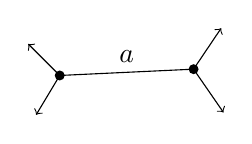
\begin{tikzpicture}[scale=1]
\fill (0,0) circle (1.8pt);\fill (1.7,0.08) circle (1.8pt);
\draw (0,0)--node[above]{$a$}(1.7,0.08);
\draw[->] (0,0)--(-.4,.4);\draw[->] (0,0)--(-.3,-.5);
\draw[->] (1.7,.08)--(2.05,.6);\draw[->] (1.7,.08)--(2.08,-.47);
\end{tikzpicture}}
correspondant à la donnée d'un ens \deleted{$\unsure{E|I}$}\inserted{$I$} de cardinal 4, et d'une partition de type $(2,2)$ de $I$, i.e. à la donnée d'un \uline{carré} combinatoire $\unsure{Q|C}$ (dont $I$ est l'ens des sommets, et la partition est celle des diagonales). \unsure{On notera|On note}
\mspage{12}

\scanpage{14}
$G_Q$ le graphe associé à un carré combinatoire $Q$,
\figure{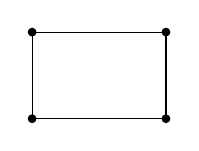
\begin{tikzpicture}\draw (0,0)--(1.7,0)--(1.7,1.1)--(0,1.1)--cycle;\fill (0,0) circle(1.6pt);\fill (1.7,0) circle(1.6pt);\fill (0,1.1) circle(1.6pt);\fill (1.7,1.1) circle(1.6pt);\end{tikzpicture}}
Soit $\operatorname{diag}Q$ l'ens des deux diagonales de $Q$; $\unsure{\mathcal A|A}(Q)$ l'ens des quatre côtés, s'identifie à
\[
\unsure{\mathcal A|A}(Q)=\prod_{\Delta\in\operatorname{diag}Q}\Delta
\]
\margin{\deleted{ens sur lequel}\inserted{torseur sous} $\{\pm1\}^{\operatorname{diag}Q}$, \deleted{qui} \unsure{donc|dont} $\{\pm1\}\subset\{\pm1\}^{\operatorname{diag}Q}$ y opère}
\deleted{\unsure{qui se}} qui se groupent \deleted{\unsure{en}} par paires de côtés opposés, en codiagonales. Alors
\[
\operatorname{codiag}(Q)\simeq\bigwedge_{\Delta\in\operatorname{diag}Q}\Delta
\]
On a ici, en termes du graphe $G_Q$
\[
\begin{aligned}
S&\simeq\operatorname{diag}Q&&\text{soit }\Delta_s\text{ la diagonale associée à }s\in S\\
I&=A^{\mathrm{lib}}=\unsure{\mathbf I|I}(Q)&&\text{ens des }\deleted{\text{côtés orientés}}\inserted{\text{sommets}}\text{ de }Q\\
\widehat{\vec A}&\simeq\mathbf I\amalg\widetilde S&&\substack{\text{en associant à }s\in S\text{ l'arête}\\\text{orientée liée }\widetilde s\text{ d'origine }s}\\
\widehat{\vec A}_s&=\Delta_s\amalg\{\widetilde s\}&&\text{donc }\varepsilon_s=\omega(\widehat{\vec A}_s)\simeq\Delta_s\\
\varepsilon_{(G)}&\simeq\prod_{s\in S}\Delta_s\simeq A(Q)&&\text{en tant que torseurs}\\
\gamma_G&=\prod_{s\in S}\{\pm1\}=\{\pm1\}^{S}.&&
\end{aligned}
\]
On trouve $S_0\mathcal T_G$ à l'aide de l'extension $\mathcal E_{G^b}$
\[
0\longrightarrow\mathbb Z^S\xrightarrow{2}\mathbb Z^S\longrightarrow\overbrace{\{\pm1\}^S}^{\gamma(G)}\longrightarrow0
\]
et du \inserted{$\gamma(G)$-torseur} $\varepsilon(G)$, en prenant $\mathcal E_{G^b}(\varepsilon(G))$, ce qui donne un $\mathbb Z^S$-\unsure{groupoïde}\inserted{sur $\gamma(G)$}, et en faisant l'extension du groupe \unsure{central} $\mathbb Z^S$ à $\mathbb Z^{\widehat{\vec A}}$, par
\mspage{13}

\scanpage{15}
l'homomorphisme
\diagram{\begin{tikzcd}[ampersand replacement=\&, column sep=large,row sep=large]
\mathbb Z^S\arrow[rr,no head]\arrow[dr,"{\substack{\text{déduit par}\\\text{contravariance}\\\text{de }\widehat{\vec A}\xrightarrow[\mathrm{or.}]{}S}}"']\&\&\mathbb Z^{\widehat A}\\
\&\mathbb Z^{\widehat{\vec A}}\arrow[ur,"{\substack{\text{déduit par}\\\text{cov. de}\\\widehat{\vec A}\longrightarrow\widehat A\simeq\widehat{\vec A}/\sigma}}"']\&
\end{tikzcd}}
\margin{\deleted{\unsure{transposé de} $\widehat{\vec A}$}$\longrightarrow S$\quad\deleted{$\vec a\mapsto$}$\operatorname{or}(\vec a)$}
Or :
\[
\mathbb Z^{\widehat A}\simeq\mathbb Z^I\times\mathbb Z,\quad\text{et}\quad\mathbb Z^S\mathbin{-}\mathbb Z^I\times\mathbb Z
\]
se décompose en
\[
\mathbb Z^S\longrightarrow\mathbb Z^I\qquad\substack{\text{associé par contravariance}\\\text{à }I\xrightarrow[\mathrm{deg}\,2]{}S}
\]
et en
\[
\mathbb Z^S\xrightarrow[\text{hom somme}]{}\mathbb Z
\]
\mspage{14}

\scanpage{16}
\uline{$\overline{\mathrm{II}}$}\quad \uline{Dé}termination de $S_0\mathcal T_{0,I}$, pour $\operatorname{card}I=4$.

Soit
\[
(1)\quad\left\{\begin{aligned}
J&=\text{ens des partitions de type }(2,2)\text{ de }I\\
\Sigma&=\mathbb P^1_J\quad\text{la }\deleted{\text{sphère}}\inserted{\text{dr. proj.}}\text{ }J\text{-marquée associée}\\
\omega&=\omega(J)\quad\text{l'ens des orientations de }J.
\end{aligned}\right.
\]
\margin{\uline{NB} $\mathfrak S_I$ opère sur $\Sigma=\Sigma_I\deleted{\unsure{(I)}}$ par l'intermédiaire de $\mathfrak S_J$, via
\diagram{\begin{tikzcd}[ampersand replacement=\&,column sep=small,row sep=small]
{}\arrow[r]\&\unsure{V(I)|V(J)}\arrow[r,no head]\&\mathfrak S_I\arrow[r]\&\mathfrak S_J\arrow[r,no head]\&0\\
\&\begin{gathered}\text{l'espace vect. de}\\\text{dim 2 sur }\mathbb F_2\\\text{déterminé}\\\text{par }J\end{gathered}\arrow[u]
\end{tikzcd}}
$V(J)^*\simeq J$}
On peut plonger $\omega$ dans $\Sigma$ par un isomorphisme
\[
(2)\qquad\omega\simeq\Sigma^{\mathfrak S_J^+}=\Sigma^{\mathfrak S_I^+}
\]
en associant à $x\in\omega$ le point fixe sous $\mathfrak S_J^+$ qui est ds l'hémisphère qui correspond à l'orientation de l'équateur $\Sigma_{\mathbb R}$ correspondant à l'ordre circulaire donné sur $J$. Pour \deleted{$\unsure{\forall}$} $\alpha\in J$, je désigne par \deleted{$\sigma_\alpha$ la transposition}
\[
\sigma_\alpha\in\mathfrak S_I
\]
la transposition dans $J$ qui fixe $\alpha$, $\widetilde\alpha$ le pt fixe $\ne\alpha$ de cette transposition.
\figure{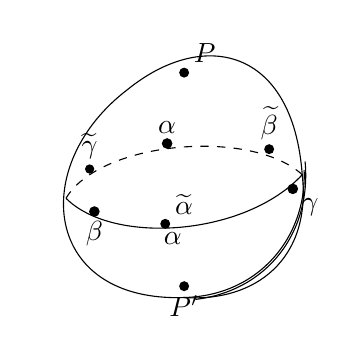
\begin{tikzpicture}[scale=1.2]
\draw (0,0) .. controls (-1.5,-.05) and (-1.65,1.4) .. (-.6,2.2) .. controls (.2,2.85) and (1.15,2.65) .. (1.25,1.3) .. controls (1.35,.4) and (.75,-.05) .. (0,0);
\draw (-1.25,1.05) .. controls (-.75,.55) and (.65,.65) .. (1.25,1.3);
\draw[dashed] (-1.25,1.05) .. controls (-.9,1.65) and (.7,1.8) .. (1.25,1.3);
\draw (.0,.0) .. controls (.8,.02) and (1.3,.65) .. (1.27,1.35);
\draw (.12,-.02) .. controls (.88,.07) and (1.35,.69) .. (1.28,1.44);
\fill (0,2.38) circle(1.5pt) node[above right]{$P$};
\fill (0,.12) circle(1.5pt) node[below]{$\unsure{P'}$};
\fill (-.18,1.63) circle(1.6pt) node[above]{$\alpha$};
\fill (-1,1.36) circle(1.4pt) node[above]{$\widetilde\gamma$};
\fill (.9,1.57) circle(1.5pt) node[above]{$\widetilde\beta$};
\fill (-.95,.91) circle(1.6pt) node[below]{$\beta$};
\fill (-.2,.78) circle(1.5pt) node[above right]{$\widetilde\alpha$};
\node[below] at(-.12,.79){$\deleted{\unsure{\alpha}}$};
\fill (1.15,1.15) circle(1.6pt) node[below right]{$\gamma$};
\end{tikzpicture}}
\margin{De façon générale, on \unsure{désignera|désigne} par $\unsure{P'|x'}$ l'\unsure{antipodique} d'un pt $P$ de $\Sigma$.}
On pose
\[
(3)\qquad\Sigma^*\deleted{\unsure{(I)}}=\Sigma_I\deleted{\unsure{\alpha(I)}}=\Sigma-\deleted{\unsure{\{}}J
\]
On a des iso. canoniques (sur $\mathbb C$)
\[
(4)\quad\left\{\begin{aligned}
M_{0,I}&\simeq\Sigma_I^*\\
\widehat M_{0,I}&\simeq\Sigma_I
\end{aligned}\right.
\]
\mspage{15}

\scanpage{17}
On prend
\[
\Sigma_J=\mathbb P(V(J))\simeq\check{\mathbb P}(V(J))
\]
où $V(J)$ défini par noyau
\[
0\mathbin{-}V(J)\longrightarrow\mathcal O^J\xrightarrow[\text{somme}]{}\mathcal O\mathbin{-}0.
\]
La section $\unsure{\alpha^*|\alpha}$ de $\Sigma_J$ est définie par le noyau
\deleted{\unsure{la section} $\unsure{\alpha}\sum_{\beta\in J\setminus\{\alpha\}}\beta$ de $V($}
\[
V(J)\xrightarrow{\operatorname{pr}_\alpha}\mathcal O
\]
qui est donné \deleted{par} loc. par \deleted{$\unsure{\alpha\mapsto\lambda\beta-\lambda\gamma}$}\inserted{$\mathcal O.(\beta-\gamma)$}, où $\beta,\gamma$ sont les élts de $J$ diff de $\alpha$. Quant à $\alpha'$, il est donné par la section
\[
-2\alpha+\beta+\gamma=-2\alpha+\sum_{\beta\in J\setminus\{\alpha\}}\beta
\]
soit $\Delta_{\alpha'}$. On a
\[
0\mathbin{-}\Delta_{\alpha'}\longrightarrow V(J)\longrightarrow\underline{\mathcal O}_{\alpha'}\unsure{(1)|\omega}\longrightarrow0
\]
\deleted{d'où}\inserted{et}
\[
\Delta_{\alpha'}\xrightarrow[\substack{\operatorname{pr}_\beta\\(\beta\ne\alpha)}]{\sim}\mathcal O.
\qquad\substack{\text{isom indépendant}\\\text{du choix de }\beta}
\]
on trouve donc, passant aux déterminants
\diagram{\begin{tikzcd}[ampersand replacement=\&, row sep=large,column sep=large]
\det V(J)\arrow[r,phantom,"\simeq"]\arrow[d,phantom,"\simeq" description]\&\underline{\mathcal O}_{\alpha'}\unsure{(1)|\omega}\\
\mathcal O^{\deleted{\unsure{\omega}}}\otimes_{\mathbb Z}\mathbb Z(\omega)\arrow[dr,bend right,"{\mathbb Z\text{ tordu par }\omega=\operatorname{or}(J)}"']\&\\
\&{}
\end{tikzcd}}
On a un isom
\[
\deleted{\unsure{\mathcal L}}\widehat T_i\simeq\deleted{\unsure{\mathcal T}}\{\mathcal O(1)\}\otimes_{\mathbb Z}L(\omega),
\]
\inserted{fibré normal de $\unsure{\widehat{\mathcal X}_{0,I}|\widehat{\mathcal C}_{0,I}}$ dans $\widehat M_{0,I}$ le long de la section $i$ $(\in I)$}
où on a l'alternative
\[
\begin{aligned}
L(\omega)&=\mathbb Z&&\text{(isom }\unsure{\text{fonctoriel}}\text{ en }\unsure{\deleted{I}J|\deleted{J}I},i\text{)}\\
L(\omega)&=\mathbb Z(\omega)&&\text{(id}\ \unsure{\}}\quad\text{où }\omega=\omega(J)\text{)}
\end{aligned}
\]
\figure{
\begin{tikzpicture}\draw (0,0)--(1.2,.05);\end{tikzpicture}}
Pour déterminer quelle est l'alternative correcte
\mspage{16}

\scanpage{18}
je prends l'image inverse par la section $\alpha'\deleted{\unsure{\Sigma}}$ $(\alpha\in J)$ de $M_{0,I}$, on aura donc
\[
\underbrace{T_i}_{\substack{\text{fibré tangent}\\\text{le long de la}\\\text{section }i\text{ de la}\\\text{sphère proj. relative}\\X\quad I\text{-marquée}}}
\simeq\underbrace{\unsure{\mathcal L|\mathcal V}\left(\underbrace{\underline{\mathcal O}_{\alpha'}(1)}_{\mathcal O\otimes_{\mathbb Z}\mathbb Z(\omega)}\right)\otimes_{\mathbb Z}L(\omega)}_{\underline{\mathcal O}\otimes_{\mathbb Z}\left(\mathbb Z(\omega)\otimes_{\mathbb Z}L(\omega)\right)}
\]
Mais on a, pour une structure carrée $Q=Q_\alpha$ sur $I$, et un sommet marqué $i$, d'où une diagonale marquée
\[
\omega(Q)\simeq\omega\deleted{\unsure{(J)}}
\]
et on trouve
\figure{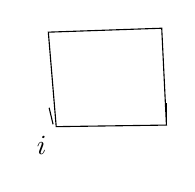
\begin{tikzpicture}\draw (0,0)--(1.4,.02)--(1.34,1.25)--(-.1,1.2)--cycle;\draw(-.04,.03)--(-.09,.24);\draw(1.4,.03)--(1.4,.3);\node[below left]at(0,0){$i$};\end{tikzpicture}}
\[
T_i\simeq\mathcal O\otimes_{\mathbb Z}\mathbb Z(\omega)
\]
et comparant, on trouve $L(\omega)=\mathbb Z$, donc en définitive
\[
\boxed{\widehat T_i\simeq\mathcal O(1)}\simeq\check F(\omega)
\]
\margin{où
\diagram{\begin{tikzcd}[ampersand replacement=\&, column sep=small]
0\arrow[r,no head]\&F\arrow[r,no head]\&V(J)_\Sigma\arrow[r]\&\underline{\mathcal O}_\Sigma(1)\arrow[d]\\
\&\&\&0
\end{tikzcd}}}
On trouve donc
\[
S\widehat P_I\overset{\mathrm{déf}}{=}\prod_{/\unsure{M_i|\widehat M}}\widehat P_i
\simeq\left(\check V^*(\mathcal O(1))\right)^{4}_{/\underbrace{\widehat M_{0,I}}_{\Sigma_I}}
\simeq V^*(\mathcal O(1))\mathbin{\wedge}_{G_m}G_m^I
\]
donc
\[
SP_I\simeq\left(V^*(\mathcal O(1))\mid\underbrace{M_{0,I}}_{\Sigma_I^*}\right)\mathbin{\wedge}_{G_m}G_m^I
\]
d'où (sur $\mathbb C$ maintenant, et dans le \unsure{contexte} analy.)
\[
S\mathcal T_{0,I}\simeq\Pi_1\left(V^*(\mathcal O(1))\mid\Sigma_I^*\right)\mathbin{\wedge}_{\mathbb Z}\mathbb Z^I
\]
\mspage{17}

\scanpage{19}
\margin{$(22\,\mathrm p)$}
Étude de $P\Sigma_J^*$

(et de $P\Sigma_n^*\ \ldots$)

$S_0\mathcal T_{0,4},\ S_0\mathcal T_{0,I}$

$(\operatorname{card}I=4)$
\mspage{18}

\scanpage{20}
\mspage{\textcircled{\unsure{0|O}}}
\figure{\begin{tikzpicture}[x=.0065cm,y=-.0065cm,>=stealth,every node/.style={font=\scriptsize}]
\draw[gray] (440,555)..controls(570,375)and(1220,356)..(1383,524)..controls(1415,620)and(1130,682)..(739,666)..controls(560,676)and(425,612)..(440,555);
\draw[gray] (440,555)--(449,1110)--(450,1725);
\draw[gray] (1383,524)..controls(1402,925)and(1392,1450)..(1396,1735);
\draw[gray] (739,666)..controls(710,1030)and(702,1530)..(685,1845);
\draw[gray] (1117,634)..controls(1152,1000)and(1080,1510)..(1076,1852);
\draw[densely dotted] (775,413)--(740,990)--(720,1618);
\draw[densely dotted] (1171,419)--(1150,973)--(1130,1608);
\draw[gray] (450,1725)..controls(575,1582)and(1160,1552)..(1396,1735)..controls(1360,1885)and(645,1918)..(450,1725);
\fill[gray] (904,535) ellipse(24 and 10);\fill[gray] (923,1730) ellipse(24 and 10);
\foreach \x/\y in {440/555,575/454,981/409,1317/454,1383/524,1300/596,739/666,539/647,509/1800,569/1646,896/1607,1305/1629,1270/1811,890/1850}{\fill(\x,\y)circle(2pt);}
\draw[->] (706,422)..controls(584,436)and(505,481)..(450,541);
\draw[->] (1137,410)..controls(1020,399)and(900,406)..(793,416);
\draw[->] (1366,498)..controls(1324,451)and(1243,433)..(1184,420);
\draw[->] (1380,575)--(1383,535);
\draw[->] (452,587)..controls(481,644)and(599,664)..(723,664);
\draw[very thick,->] (754,669)..controls(904,671)and(1007,652)..(1112,635);
\draw[very thick,->] (1135,647)--(1125,1229);
\draw[->] (1161,896)--(1151,963);\draw[->] (749,922)--(738,984);
\draw[->] (446,1040)--(452,1103);\draw[->] (447,1190)--(445,1129);
\draw[->] (1399,1024)--(1407,1080);\draw[->] (1405,1175)--(1410,1120);
\draw[->] (728,1150)--(715,1222);\draw[->] (707,1304)--(709,1244);
\draw[->] (1136,1312)--(1126,1250);
\draw[->] (693,1607)--(710,1617);\draw[->] (1102,1606)--(1122,1605);
\draw[->] (500,1792)..controls(472,1776)and(445,1754)..(439,1728);
\draw[->] (879,1853)--(701,1850);\draw[->] (1276,1807)..controls(1226,1826)and(1159,1838)..(1095,1846);
\draw[->] (1398,1672)..controls(1433,1707)and(1411,1743)..(1405,1756);
\draw[->] (1060,1825)--(898,1825);
\draw[->] (1452,540)..controls(1507,506)and(1487,452)..(1411,421);
\draw[->] (347,1742)..controls(305,1700)and(319,1659)..(396,1673);
\foreach \x/\y in {550/1034,950/980,1335/1005,530/1215,892/1248,1342/1180}{\fill[gray](\x,\y)circle(4pt);}
\draw[->] (512,1023)..controls(509,962)and(557,963)..(572,1007);
\draw[->] (585,1040)..controls(591,1081)and(533,1105)..(516,1062);
\draw[->] (583,1045)..controls(583,1081)and(530,1082)..(520,1070);
\draw[->] (910,965)..controls(923,915)and(967,920)..(985,960);
\draw[->] (989,988)..controls(990,1030)and(929,1020)..(910,991);
\draw[->] (1295,989)..controls(1320,947)and(1370,953)..(1374,1019);
\draw[->] (1370,1032)..controls(1339,1070)and(1308,1069)..(1292,1018);
\draw[->] (1364,1030)..controls(1311,1063)and(1304,1048)..(1293,1022);
\draw[->] (489,1200)..controls(500,1154)and(563,1164)..(576,1215);
\draw[->] (485,1224)..controls(480,1290)and(542,1283)..(574,1239);
\draw[->] (1330,1133)..controls(1307,1129)and(1280,1164)..(1286,1189);
\draw[->] (1281,1204)..controls(1266,1268)and(1367,1244)..(1383,1160);
\draw[->] (1381,1148)..controls(1373,1129)and(1350,1124)..(1330,1133);
\draw[gray] (450,1110)--(930,1090)--(1410,1105)--(530,1215)--(930,1090)--(1342,1180);
\draw[gray] (930,1090)--(710,1238);\draw[gray] (930,1090)--(844,1235);\draw[gray] (930,1090)--(944,1235);\draw[gray] (930,1090)--(1124,1238);
\begin{scope}\clip (930,1090)--(844,1235)--(1124,1238)--cycle;\foreach \t in {650,675,...,1200}{\draw[gray](\t,1250)--(\t+220,1050);}\end{scope}
\begin{scope}\clip (930,1090)--(530,1215)--(710,1238)--cycle;\foreach \t in {550,575,...,900}{\draw[gray](\t,1250)--(\t+25,1100);}\end{scope}
\draw[->] (457,1093)--(505,1051);\draw[->] (692,997)--(580,1028);
\draw[->] (755,991)--(900,978);\draw[->] (1110,970)--(998,973);
\draw[->] (1160,976)--(1288,989);\draw[->] (1379,1043)--(1402,1084);
\draw[->] (450,1131)--(485,1190);\draw[->] (692,1236)--(578,1227);
\draw[->] (725,1237)--(837,1239);\draw[very thick,->] (1111,1236)--(953,1240);
\draw[very thick,->] (943,1236)..controls(915,1179)and(872,1179)..(843,1235);
\draw[->] (845,1259)..controls(872,1300)and(923,1300)..(943,1258);
\draw[->] (1150,1237)--(1284,1203);\draw[->] (1398,1130)--(1376,1167);
\node[right]at(1540,500){$V_{\mathbb C}^{\omega}$};\node[right]at(1530,1080){$V_\omega$};\node[right]at(1503,1715){$V_{\mathbb C}^{\omega'}$};
\node[left,text=gray]at(353,568){$\unsure{O_\omega}$};\node[left,text=gray]at(356,1150){$\unsure{O}$};\node[left,text=gray]at(271,1770){$\unsure{O_{\omega'}}$};
\node[below left]at(739,666){$\widetilde P_{a_1}^{\omega}$};\node[below]at(940,669){$\widetilde P_s^{\omega}$};\node[below left]at(1117,634){$\widetilde P_a^{\omega}$};
\node[above]at(857,651){$\widetilde d_r^{\omega}$};\node[above]at(938,637){$\deleted{\unsure{\widetilde d_s^{\omega}}}$};\node[above]at(1018,640){$\widetilde d_s^{\omega}$};\node[above]at(1125,615){$\deleted{\unsure{\widetilde P_a^{\omega}}}$};
\node[left]at(745,910){$\widetilde c_{a_1}^{\omega}=\widetilde c_{\omega^{-1}(r)}$};\node[left]at(1130,887){$\unsure{\widetilde C_r|\widetilde c_r}\text{ ou }\widetilde C_a^{\omega}$};
\node[below left]at(710,1238){$\widetilde Q_{a_1}$};\node[below right]at(1124,1238){$\widetilde Q_a$};
\node[below left]at(844,1240){$\widetilde R_{r_1}$};\node[below]at(892,1248){$\widetilde R_s$};\node[below right]at(946,1240){$\widetilde R_r$};
\node[above]at(780,1229){$\widetilde b_{r_1}$};\node[above]at(1050,1229){$\widetilde b_r$};\node[above]at(896,1209){$\widetilde a_r$};
\node at(967,1136){$r$};\node at(1032,1137){$r'$};\node at(1082,1106){$r''$};\node at(817,1152){$r_2$};
\node at(777,1150){$\deleted{\unsure{\omega(r)}}$};\node at(851,1125){$\deleted{\unsure{r'}}$};\node at(863,1160){$\deleted{\unsure{r_1}}$};\node at(988,1178){$\deleted{\unsure{r}}$};\node at(1080,1165){$\deleted{\unsure{r}}$};\node at(1285,1126){$\deleted{\unsure{\omega\omega(r)}}$};
\node[left]at(721,1530){$\widetilde c_{r_1}=\widetilde c_{a_1}^{\omega'}$};
\node[below]at(690,1853){$\widetilde P_{a_1}^{\omega'}$};\node[below]at(891,1860){$\widetilde P_s^{\omega}$};\node[below]at(1081,1858){$\unsure{\widetilde P_a^{\omega'}|\widetilde Q_a^{\omega'}}$};
\node[above]at(978,1825){$\widetilde b_r^{\omega'}$};\node[below]at(787,1867){$(\unsure{\widetilde d_{r'}^{\omega}|\widetilde d_r^{\omega'}})$};
\node[below]at(997,1878){$\deleted{\unsure{\widetilde d_s^{\omega'}}}$};\node[below]at(997,1934){$\unsure{\widetilde d_{r_1}\text{ ou }\widetilde d_s^{\omega'}}$};
\node[anchor=west,align=left]at(40,930){$\begin{aligned}
s&\in S\\a&\in A\\r&=(s,a)\\r_1&=(s,\unsure{a_1})=\tau_A r\\r_2&=\omega^{-1}(r)=\tau_0\tau_A\deleted{\unsure{r}}=\tau_0\tau_A r\\
&\deleted{\unsure{r'}=\omega(r)=\tau_0(\tau_1r)}\\
r'&=\tau_0r\\r''&=\unsure{\tau_A|\tau_1}r'=\tau_1\tau_0r=\omega(r))
\end{aligned}$};
\end{tikzpicture}}
\mspage{19}

\scanpage{21}
\mspage{20}
\begin{center}
U N I V E R S I T E\\
DES SCIENCES ET TECHNIQUES\\
DU LANGUEDOC\\
------------\\
Service de la Scolarité\\
MR/IE\\
\uline{Diffusion} : Liste A\\
N$^\circ$ 2090
\end{center}
Montpellier, le 2 avril 1980

\begin{center}
\uline{AVIS DE SOUTENANCE D'UNE THESE DE DOCTORAT DE SPECIALITE} :\\
\uline{CHIMIE ORGANIQUE PHYSIQUE}
\end{center}
\uline{Nom et Prénom} : MARCHETTI Jacqueline épouse SMADJA

\uline{Titre de la thèse} : Résolution cinétique et détermination du pouvoir rotatoire spécifique
de cétones chirales

\uline{Date, heure et lieu de soutenance prévus} : 10 avril 1980 à 10 heures ; U.E.R. des Sciences,
Centre Universitaire de la Réunion

\uline{Nom du Directeur de la thèse} : Messieurs Gérard LAMATY et Jacques CONAN

\uline{Désignation du laboratoire où la thèse est préparée} :
Laboratoire de Chimie Organique Centre Universitaire de la Réunion

\uline{Analyse de l'ouvrage} :
Un certain nombre de dioxolannes-1,3 diastéréoisomères ont été synthétisés à partir de cétones
chirales et de diols optiquement actifs dérivés de l'acide R-R tartrique.

Les constantes de vitesse d'hydrolyse de ces dioxolannes ont été mesurées ainsi que l'évolu-
tion, en fonction du temps, du pouvoir rotatoire de la cétone obtenue. A partir de ces deux
données on déduit le pouvoir rotatoire spécifique des cétones et les meilleures conditions
d'obtention de produits optiquement actifs.

\uline{Durée approximative des recherches ayant abouti à la thèse} : 4 ans.

\uline{Composition du jury proposé} : MM. : LAMATY Gérard\\
LATTES Armand\\
CARBONEL Max\\
ROQUE J.P.\\
CONAN Jacques

P/le Secrétaire Général\\
L'Attachée d'Administration Universitaire,

\figure{
\begin{tikzpicture}[x=.8cm,y=.8cm]
\draw (0,.1) .. controls (-.18,.55) and (.35,.7) .. (.65,.65);
\draw (.65,.65) .. controls (.25,.69) and (-.1,.34) .. (.08,.2) .. controls (.3,.01) and (.8,.13) .. (.49,.31) .. controls (.35,.36) and (.33,.13) .. (.77,.22);
\draw (.54,.22) .. controls (1,.25) and (.8,.16) .. (1.05,.19)--(1.49,.2);
\draw (1.6,.22) .. controls (1.91,.1) and (1.94,.41) .. (1.92,.62);
\draw (1.94,.68)--(1.98,.9);
\draw (.03,.73)--(0,.91);
\draw (.15,-.05)--(2.95,-.04);
\end{tikzpicture}}
\uline{A. GENTIL.}

MR LE PROFESSEUR GROTHENDIECK ALEX.

MATHEMATIQUES\hfill 5

\scanpage{22}
\mspage{21}
\figure{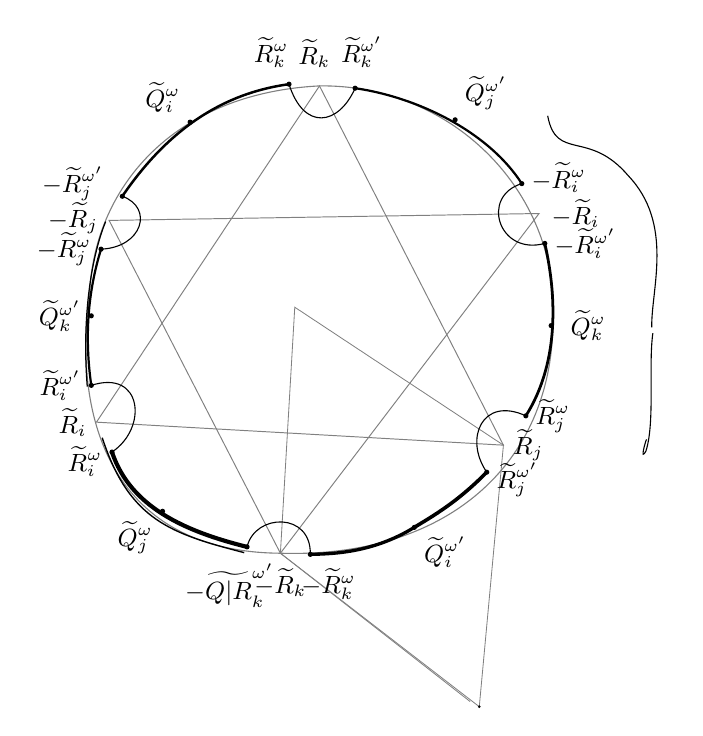
\begin{tikzpicture}[x=.73cm,y=.73cm,every node/.style={font=\small}]
\draw[gray,line width=.35pt] (2.22,7.01)--(9.7,7.13)--(5.2,1.22)--cycle;
\draw[gray,line width=.35pt] (5.88,9.35)--(2.0,3.5)--(9.08,3.1)--cycle;
\draw[gray,line width=.3pt] (5.45,5.5)--(9.08,3.1)--(8.66,-1.45)--(5.2,1.22)--cycle;
\draw[gray,line width=.3pt] (5.2,1.22)--(8.5,-1.36);
\draw[gray] (5.88,9.35) .. controls (8.25,9.38) and (10.1,7.42) .. (9.94,5.2) .. controls (9.91,2.78) and (8.11,1.13) .. (5.2,1.22) .. controls (2.28,1.24) and (1.58,3.55) .. (1.88,5.7) .. controls (1.94,7.54) and (3.3,9.22) .. cycle;
\draw[line width=.9pt] (2.45,7.43) .. controls (3.45,8.9) and (4.56,9.27) .. (5.35,9.38);
\draw[line width=.8pt] (6.5,9.31) .. controls (7.6,9.15) and (8.82,8.55) .. (9.4,7.65);
\draw[line width=1pt] (9.8,6.61) .. controls (10.03,5.6) and (10.02,4.48) .. (9.47,3.61);
\draw[line width=1.3pt] (8.79,2.63) .. controls (8.27,2.1) and (7.84,1.86) .. (7.53,1.67);
\draw[line width=1.2pt] (7.53,1.67) .. controls (6.8,1.22) and (6.1,1.21) .. (5.72,1.2);
\draw[line width=1.5pt] (4.62,1.33) .. controls (3.54,1.6) and (2.59,2.02) .. (2.27,2.98);
\draw[line width=.8pt] (1.91,4.14) .. controls (1.79,4.98) and (1.85,5.77) .. (2.08,6.51);
\draw[line width=.5pt] (4.57,1.23) .. controls (3.3,1.56) and (2.57,1.79) .. (2.1,3.23);
\draw[line width=.45pt] (1.84,4.12) .. controls (1.74,5.4) and (1.93,6.43) .. (2.16,6.99);
\draw (5.35,9.38) .. controls (5.61,8.56) and (6.21,8.66) .. (6.5,9.31);
\draw (2.45,7.43) .. controls (3.0,7.23) and (2.8,6.54) .. (2.08,6.51);
\draw (1.91,4.14) .. controls (2.8,4.43) and (2.9,3.4) .. (2.27,2.98);
\draw (4.62,1.33) .. controls (4.76,1.92) and (5.74,1.94) .. (5.72,1.2);
\draw (8.79,2.63) .. controls (8.39,3.21) and (8.71,3.96) .. (9.47,3.61);
\draw (9.4,7.65) .. controls (8.67,7.43) and (9.0,6.39) .. (9.8,6.61);
\foreach \p in {(5.35,9.38),(6.5,9.31),(2.45,7.43),(2.08,6.51),(1.91,4.14),(2.27,2.98),(4.62,1.33),(5.72,1.2),(8.79,2.63),(9.47,3.61),(9.4,7.65),(9.8,6.61),(3.63,8.72),(8.24,8.76),(9.91,5.18),(7.53,1.67),(3.15,1.95),(1.91,5.35)}{\fill \p circle(.045);}
\fill (8.66,-1.45) circle(.025);
\node[above] at (5.04,9.5) {$\widetilde R_k^\omega$};
\node[above] at (5.79,9.5) {$\widetilde R_k$};
\node[above] at (6.62,9.5) {$\widetilde R_k^{\omega'}$};
\node[above left] at (3.63,8.72) {$\widetilde Q_i^\omega$};
\node[above right] at (8.24,8.76) {$\widetilde Q_j^{\omega'}$};
\node[left] at (2.3,7.65) {$-\widetilde R_j^{\omega'}$};
\node[left] at (2.2,7.05) {$-\widetilde R_j$};
\node[left] at (2.08,6.51) {$-\widetilde R_j^\omega$};
\node[left] at (1.91,5.35) {$\widetilde Q_k^{\omega'}$};
\node[left] at (1.91,4.14) {$\widetilde R_i^{\omega'}$};
\node[left] at (2.0,3.5) {$\widetilde R_i$};
\node[left] at (2.27,2.82) {$\widetilde R_i^\omega$};
\node[below left] at (3.15,1.95) {$\widetilde Q_j^\omega$};
\node[below] at (4.32,1.2) {$-\widetilde{\unsure{Q|R}}_k^{\omega'}$};
\node[below] at (5.2,1.12) {$-\widetilde R_k$};
\node[below] at (6.04,1.12) {$-\widetilde R_k^\omega$};
\node[below right] at (7.53,1.67) {$\widetilde Q_i^{\omega'}$};
\node[right] at (8.79,2.5) {$\widetilde R_j^{\omega'}$};
\node[right] at (9.08,3.1) {$\widetilde R_j$};
\node[right] at (9.47,3.61) {$\widetilde R_j^\omega$};
\node[right] at (10.08,5.18) {$\widetilde Q_k^\omega$};
\node[right] at (9.4,7.75) {$-\widetilde R_i^\omega$};
\node[right] at (9.75,7.13) {$-\widetilde R_i$};
\node[right] at (9.8,6.61) {$-\widetilde R_i^{\omega'}$};
\draw (9.85,8.83) .. controls (10.0,8.03) and (10.56,8.6) .. (11.25,7.79) .. controls (12.05,6.95) and (11.65,5.82) .. (11.66,5.15);
\draw (11.68,5.05) .. controls (11.6,4.5) and (11.72,3.5) .. (11.56,3.0) .. controls (11.45,2.8) and (11.55,3.17) .. (11.57,3.2);
\end{tikzpicture}}
NB $\omega_{ij}$ est l'orientation telle que
$\omega_{ij}(j)=i$
\[
(\{i,j,k\}=J)\qquad
\widetilde R_i^{\unsure{\omega}}=(e_j-e_k)\mathbin{\wedge}\omega_{jk}
\]
\[
\widetilde Q_i^\omega=\widetilde R_{\omega^2\unsure{i}}-\widetilde R_{\omega i}
\]
donc
\[
i_\omega\widetilde Q_i^\omega=\widetilde R_i
\]
\[
i_\omega\widetilde R_i=-\widetilde Q_i^\omega=\widetilde Q_i^{\omega'}
\]
\[
\widetilde Q_i^\omega=(e_j+e_k-2e_i)\mathbin{\wedge}\omega
\]

\scanpage{23}
\mspage{22}
\begin{center}
UNIVERSITÉ DES SCIENCES\\
ET TECHNIQUES DU LANGUEDOC\\
MONTPELLIER II\\
Place Eugène Bataillon\\
34060 MONTPELLIER CEDEX\\
---
\end{center}
Tél. : 63.91.44 -- Télex : USTMONT 49944 F

ACADÉMIE DE MONTPELLIER
\begin{center}--------\end{center}
FA/RR

Service Général

Montpellier, le 6 Mars\hfill 19 79

\begin{center}\uuline{A D D I T I F}\end{center}

Comme suite à notre lettre du 28 Février 1979
(n$^\circ$ 01176 - Diffusion : Liste A - Directeurs de Laboratoires
propres et d'Equipe de Recherche) et en complément à notre
envoi, veuillez trouver ci-joint :

- Renseignements pratiques.\\
- Organigramme

concernant le "Questionnaire Bilan".

\begin{center}---\end{center}

\scanpage{24}
\mspage{23}
\figure{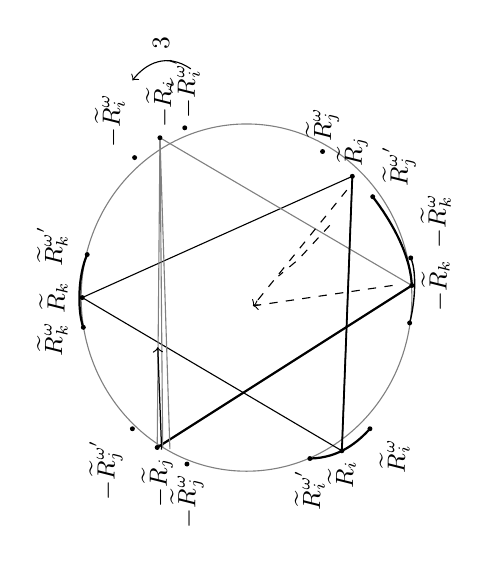
\begin{tikzpicture}[x=.7cm,y=.7cm,every node/.style={font=\small}]
\begin{scope}[rotate=90,transform shape]
\draw[gray] (0,0) ellipse (3.15 and 3.0);
\draw (0,2.98)--(-2.78,-1.73)--(2.2,-1.92)--cycle;
\draw[gray] (-2.72,1.62)--(2.9,1.57)--(.22,-3.0)--cycle;
\draw[line width=.8pt] (-2.72,1.62)--(.22,-3.0);
\draw[line width=.65pt] (-2.78,-1.73)--(2.2,-1.92);
\draw[gray,line width=.4pt] (-2.72,1.52)--(2.9,1.57);
\draw[gray,line width=.4pt] (-2.75,1.39)--(2.9,1.57);
\draw[->,line width=.45pt] (-2.76,1.54)--(-.9,1.61);
\draw[line width=.8pt] (-.54,2.96)..controls(-.25,3.07)and(.41,3.06)..(.78,2.89);
\draw[line width=.8pt] (-2.92,-1.15)..controls(-2.91,-1.7)and(-2.6,-2.04)..(-2.38,-2.24);
\draw[line width=.8pt] (1.83,-2.29)..controls(1.41,-2.61)and(.81,-2.97)..(.22,-3.0);
\draw[line width=.5pt] (-.46,-2.96)..controls(-.13,-3.05)and(.45,-3.1)..(.72,-2.98);
\draw[->,dashed] (.22,-2.65)--(-.15,-.12);
\draw[->,dashed] (1.95,-1.82)--(-.15,-.12);
\draw[dashed] (1.31,-1.51)--(.69,-.94)--(.39,-.58);
\foreach \p in {(-.54,2.96),(0,2.98),(.78,2.89),(-2.38,2.07),(-2.72,1.62),(-3.02,1.08),(-2.92,-1.15),(-2.78,-1.73),(-2.38,-2.24),(-.46,-2.96),(.22,-3.0),(.72,-2.98),(1.83,-2.29),(2.2,-1.92),(2.65,-1.38),(2.54,2.03),(2.9,1.57),(3.08,1.12)}{\fill \p circle(.045);}
\node[above] at (-.75,3.07) {$\widetilde R_k^\omega$};
\node[above] at (0,3.07) {$\widetilde R_k$};
\node[above] at (.94,3.07) {$\widetilde R_k^{\omega'}$};
\node[above left] at (-2.38,2.07) {$-\widetilde R_j^{\omega'}$};
\node[left] at (-2.72,1.62) {$-\widetilde R_j$};
\node[left] at (-3.02,1.08) {$-\widetilde R_j^\omega$};
\node[left] at (-2.92,-1.15) {$\widetilde R_i^{\omega'}$};
\node[left] at (-2.78,-1.73) {$\widetilde R_i$};
\node[below left] at (-2.38,-2.24) {$\widetilde R_i^\omega$};
\node[below] at (.22,-3.0) {$-\widetilde R_k$};
\node[below right] at (.72,-2.98) {$-\widetilde R_k^\omega$};
\node[below right] at (1.83,-2.29) {$\widetilde R_j^{\omega'}$};
\node[right] at (2.2,-1.92) {$\widetilde R_j$};
\node[right] at (2.65,-1.38) {$\widetilde R_j^\omega$};
\node[above right] at (2.54,2.03) {$-\widetilde R_i^\omega$};
\node[right] at (2.9,1.57) {$-\widetilde R_i$};
\node[right] at (3.08,1.12) {$\unsure{-}\widetilde R_i^{\unsure{\omega'}}$};
\draw[->] (4.15,1.01)..controls(4.45,1.45)and(4.25,1.83)..(3.94,2.07);
\node[right] at (4.32,1.55) {$3$};
\end{scope}
\end{tikzpicture}}

\figure{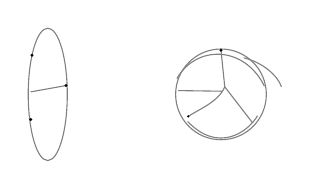
\begin{tikzpicture}[x=.8cm,y=.8cm]
\draw[gray] (0,0) ellipse (.31 and 1.05);
\draw[gray] (-.27,.04)--(.29,.14);
\fill (-.25,.62) circle(.025);\fill(-.27,-.4)circle(.025);\fill(.29,.14)circle(.025);
\begin{scope}[xshift=2.2cm]
\draw[gray] (0,0) circle(.72);
\draw[gray] (-.7,.25)..controls(-.4,.78)and(.36,.79)..(.69,.13);
\draw[gray](-.53,-.43)..controls(-.03,-.95)and(.44,-.58)..(.58,-.34);
\draw[gray](0,.7)--(.06,.12)--(.5,-.45);
\draw[gray](.06,.12)..controls(-.04,-.12)and(-.34,-.23)..(-.52,-.35);
\draw[gray](-.68,.06)--(.02,.05);
\draw[gray](.36,.58)..controls(.66,.51)and(.9,.3)..(.96,.12);
\fill (0,.7)circle(.025);\fill(-.52,-.35)circle(.02);
\end{scope}
\end{tikzpicture}}

\figure{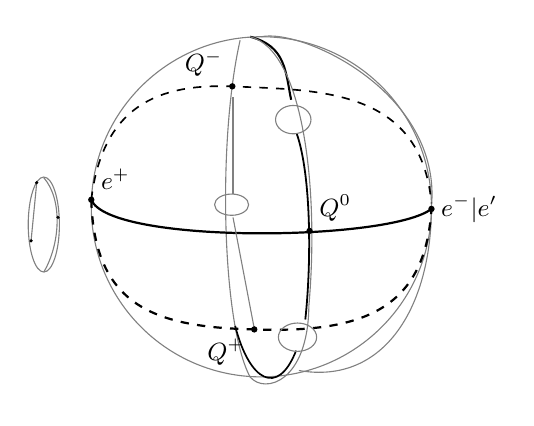
\begin{tikzpicture}[x=.9cm,y=.9cm,every node/.style={font=\small}]
\draw[gray] (0,0) circle(2.4);
\draw[gray] (0,2.4)..controls(.58,2.52)and(2.55,1.61)..(2.4,0)..controls(2.4,-1.4)and(1.74,-2.52)..(.53,-2.31);
\draw[gray](-.3,2.35)..controls(-.62,.95)and(-.56,-1.65)..(-.16,-2.4);
\draw[line width=.75pt](-.16,2.4)..controls(.35,2.27)and(.34,1.9)..(.42,1.51);
\draw[line width=.65pt](.5,1.03)..controls(.7,.45)and(.71,-.75)..(.62,-1.59);
\draw[line width=.6pt](.49,-2.03)..controls(.23,-2.69)and(-.17,-2.46)..(-.37,-1.68);
\draw[gray](-.16,2.4)..controls(.58,2.22)and(.82,.3)..(.67,-1.4)..controls(.66,-2.47)and(.05,-2.65)..(-.16,-2.4);
\draw[dashed,line width=.6pt](-2.4,.1)..controls(-2.23,1.54)and(-1.3,1.73)..(-.41,1.7)..controls(.76,1.64)and(2.25,1.7)..(2.4,.05);
\draw[line width=.8pt](-2.4,.1)..controls(-2.15,-.53)and(1.8,-.49)..(2.4,-.03);
\draw[dashed,line width=.8pt](-2.4,.1)..controls(-2.36,-1.41)and(-1.49,-1.7)..(-.1,-1.73)..controls(1.37,-1.78)and(2.31,-1.49)..(2.4,-.03);
\draw[gray](-.42,.03)ellipse(.24 and .15);
\draw[gray](.45,1.23)ellipse(.25 and .2);
\draw[gray](.51,-1.84)ellipse(.27 and .2);
\draw[gray](-.4,.18)--(-.4,1.55);
\draw[gray](-.4,-.15)--(-.1,-1.72);
\foreach \p in {(-2.4,.1),(2.4,-.03),(.68,-.34),(-.41,1.7),(-.1,-1.73)}{\fill\p circle(.045);}
\node[above right]at(-2.4,.1){$e^+$};
\node[right]at(2.4,-.03){$\unsure{e^-|e'}$};
\node[above right]at(.68,-.34){$\unsure{Q}^0$};
\node[above left]at(-.41,1.7){$\unsure{Q}^-$};
\node[below left]at(-.1,-1.73){$\unsure{Q}^{\unsure{+}}$};
\draw[gray](-3.07,-.25)ellipse(.22 and .67);
\draw[gray](-3.07,.41)..controls(-2.8,.1)and(-2.84,-.53)..(-3.07,-.92);
\draw[gray](-3.25,-.48)--(-3.17,.34);
\fill(-3.17,.34)circle(.025);\fill(-3.25,-.48)circle(.025);\fill(-2.87,-.15)circle(.025);
\end{tikzpicture}}

\figure{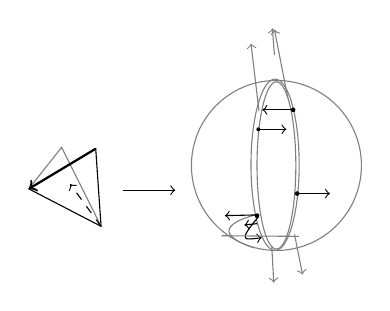
\begin{tikzpicture}[x=.85cm,y=.85cm]
\draw (-3.1,.1)--(-2.1,.7)--(-2.02,-.46)--cycle;
\draw[gray](-3.1,.1)--(-2.61,.72)--(-2.02,-.46);
\draw[->,line width=.8pt](-2.1,.7)--(-3.1,.1);
\draw[->,dashed](-2.02,-.46)--(-2.48,.17);
\draw[->](-1.69,.08)--(-.91,.08);
\draw[gray](.6,.45)circle(1.27);
\draw[gray](.6,.45)ellipse(.29 and 1.25);
\draw[gray](.58,.46)ellipse(.36 and 1.28);
\draw[->](.31,-.42)--(.12,-.44);
\draw[->](.91,.03)--(1.4,.03);
\draw[->](.85,1.28)--(.39,1.28);
\draw[->](.33,.99)--(.75,.99);
\draw[->,gray](.53,-.75)--(.56,-1.3);
\draw[->,gray](.87,-.58)--(.99,-1.18);
\draw[->,gray](.34,1.26)--(.22,2.27);
\draw[->,gray](.77,1.46)--(.57,2.48);
\draw[->,gray](.57,2.1)--(.54,2.5);
\draw[gray](.28,-.29)..controls(-.23,-.43)and(-.24,-.61)..(.26,-.78);
\draw[->](.28,-.29)--(-.17,-.3);
\draw[->](.33,-.32)..controls(.01,-.7)and(.12,-.66)..(.38,-.63);
\draw[gray](-.22,-.6)--(.94,-.61);
\fill(.31,-.3)circle(.035);\fill(.91,.03)circle(.035);\fill(.85,1.28)circle(.035);\fill(.33,.99)circle(.03);
\end{tikzpicture}}

\scanpage{25}
\margin{24}
\begin{center}- 2 -\end{center}
\begin{flushright}
MR LE PROFESSEUR GROTHENDIECK ALEX.\\
MATHEMATIQUES \hfill 5
\end{flushright}

Ces documents doivent \uline{impérativement} me parvenir, datés et signés par chaque chef de projet, \uline{avant le 15 mai prochain} à l'adresse suivante :

\begin{center}
Ministère des Universités\\
Délégation aux Relations Universitaires\\
Internationales\\
Bureau des Echanges Scientifiques\\
173, boulevard Saint-Germain\\
75006 PARIS
\end{center}

Il peut s'agir :

1) De projets nouveaux pour lesquels les moyens sont accordés annuellement (les demandes ponctuelles ne relevant pas des projets intégrés).

2) De projets en cours. Il est rappelé que la demande de moyens doit être renouvelée chaque année. Outre le dossier ci-joint, vous voudrez bien me faire parvenir un bilan détaillé faisant apparaître l'état d'avancement du projet, les résultats obtenus et les perspectives de développement de la coopération..

Les responsables français sont tenus d'une part de présenter un projet, même si les responsables québécois, ont, de leur côté, établi un projet parallèle, d'autre part, de mentionner les noms et qualités des personnes impliquées.

J'appelle votre attention sur la possibilité d'accorder à compter de cette année de nouveaux moyens (délégation de courte ou longue durée) en application du décret n\textsuperscript{o} 78-216 du 2 mars 1978 relatif au régime de certaines positions des personnels enseignants titulaires de statut universitaire.

Je vous précise enfin que cette circulaire ne concerne pas les projets d'enseignement et de recherche en médecine, pharmacie, agronomie, pour lesquels les procédures sont différentes. A ce sujet, vous voudrez bien vous référer à la note ci-annexée.

\begin{flushright}
Pour le Ministre\\
et par \unsure{délégation}\\
Le \unsure{Délégué aux Relations}\\
\unsure{Universitaires Internationales}\\
\unsure{P. T.}\\
Pierre TABATONI
\end{flushright}

\margin{La présente circulaire sera publiée au Bulletin Officiel du Ministère de l'Education et du Ministère des Universités}

\hrule
\medskip
DIFFUSION, liste C, n\textsuperscript{o} 1874, NC.PB

MONTPELLIER, le 27 Mars 1979

Le Délégué aux Relations Internationales,

\unsure{F. Schué}

\uline{F. SCHUE}

\begin{flushright}
Transmis par la Cellule des Relations\\
Internationales\\
(Mme CAPELLE, poste 315) où vous pourrez\\
consulter les annexes et retirer un formulaire de présentation de projet.
\end{flushright}

\scanpage{27}
\mspage{1}
\margin{26}
\[
\left(\begin{gathered}
r=(s,a\deleted{\unsure{,\omega}})\quad\hbox{ou }(s,a,\omega)\\
r'=\sigma_0r=(s,a')
\end{gathered}\right)
\]
\diagram{
\begin{array}{c|ll|l}
\unsure{a_r}&\longmapsto\ \widetilde a_r:\widetilde R_r\longrightarrow\widetilde R_{r'}&r\in R&\\
b_r&\mathrel{\longleftarrow\!\vert}\ \widetilde b_r:\widetilde Q_a\longrightarrow\widetilde R_r&r\in R&\left.\vphantom{\begin{array}{c}1\\1\\1\end{array}}\right\}\ \text{flèches ``\unsure{obliques}''}\\
c_a&\mathrel{\longleftarrow\!\vert}\ \widetilde c_a^\omega:\widetilde P_a^\omega\longrightarrow\widetilde Q_a&(a,\omega)\in A\times\underline\omega\simeq R&\\
&\text{ou }\widetilde c_r&&\\
1&\mathrel{\longleftarrow\!\vert}\ \lambda_{\widetilde P_a^\omega}\quad\text{lacet en }\widetilde P_a^\omega,\ \deleted{\unsure{\lambda}}&(a,\omega)\in A\times\underline\omega\simeq R&\\
1&\mathrel{\longleftarrow\!\vert}\ \lambda_{\widetilde Q_a}^{\deleted{\unsure{\omega}}}\quad\text{lacet en }\widetilde Q_a&(a,\deleted{\unsure{\omega}})\in A\deleted{\unsure{\times\underline\omega\simeq R}}&\\
1&\mathrel{\longleftarrow\!\vert}\ \lambda_{\widetilde R_r}\quad\text{lacet en }\widetilde R_r&r\in R&\\
\unsure{1}&\mathrel{\longleftarrow\!\vert}\ \mu_{\widetilde Q_a^{\deleted{\unsure{\omega}}}}^{\deleted{\unsure{\omega}}}:\widetilde Q_a\longrightarrow\deleted{\unsure{a\omega}}(\widetilde Q_a^\vee)&(a,\deleted{\unsure{\omega}})\in A\deleted{\unsure{\simeq R}}&\text{flèches ``fibres''}\\
1&\mathrel{\longleftarrow\!\vert}\ \mu_{\widetilde R_r}:\widetilde R_r\longrightarrow\deleted{\unsure{a\omega}}\widetilde R_r^\vee&r\in R&\text{ou ``verticales''}\\
1&\mathrel{\longleftarrow\!\vert}\ \widetilde d_{\unsure{r}}^{\unsure{\omega}}:\widetilde P_{a_1}^\omega\longrightarrow\widetilde P_a^\omega&r\unsure{=}(s,\omega)\in S\times\underline\omega\simeq R&\\
&\text{ou }\widetilde d_s^\omega&&
\end{array}
}
\inserted{\unsure{renversent l'ordre}}
\inserted{\unsure{renv. l'ordre}}
\margin{\deleted{\(\unsure{\lambda_{\widetilde Q_a}}\)}\quad\deleted{\(\unsure{\lambda_{\widetilde R_r}}\)}\quad\deleted{\(\unsure{\mu_{\widetilde Q_a}^\omega}\)}\quad\deleted{\(\unsure{\mu_{\widetilde R_r}^\omega}\)}\quad\deleted{\unsure{\(\omega\) quelconque}}}

\diagram{
\begin{array}{c|ll}
P^\omega&\mathrel{\longleftarrow\!\vert}\widetilde P_a^\omega&(a,\omega)\in A\underline\omega\simeq R\\
Q_a&\mathrel{\longleftarrow\!\vert}\widetilde Q_a&a\in A\\
R_r&\mathrel{\longleftarrow\!\vert}\widetilde R_r&r\in R
\end{array}
}
\margin{\unsure{renv. l'ordre}}
\margin{\deleted{\unsure{1}}}

``relations mixtes''
\[
\textcircled{1}\quad
\widetilde a_r\widetilde b_r\widetilde c_r\widetilde d_r
=\widetilde b_{\unsure{r_1'}}\widetilde c_{\unsure{a_1}}^{\unsure{\omega}}
\qquad
\underline{r\in R},\quad r'=\sigma_0r,\quad
r_1=\sigma_1\sigma_0(r')=\omega'r'.
\]

``relations fibres''
\[
\left\{\begin{array}{ll}
(5)\deleted{\unsure{(2)}}&\widetilde d_{\omega^m r}\cdots\widetilde d_{\omega r}\widetilde d_r=\lambda_{\widetilde P_{\unsure{a'_1}}^\omega}\\
(6)&\unsure{\times}\,\mu_{\widetilde Q_{\unsure{a^\vee}}}^{\deleted{\unsure{\omega}}}\mu_{\widetilde Q_a}^{\deleted{\unsure{\omega}}}=\lambda_{\widetilde Q_a}^{\deleted{\unsure{\omega}}}\\
(7)&\unsure{\times}\,\mu_{\widetilde R_{r\deleted{\unsure{,\omega}}}^\vee}\mu_{\widetilde R_r}=\lambda_{\widetilde R_r}
\end{array}\right.
\quad
\begin{array}{l}
\underline{r\in R},\quad r=(s,a,\omega),\quad a'=\omega^{-1}(a):\\
(a\deleted{\unsure{,\omega}})\in A\deleted{\unsure{\times\underline\omega\simeq R}}\\
r\in R
\end{array}
\]

``relations de transport'' ou ``de commutation''
\[
\left\{\begin{array}{lll}
(8)&\widetilde a_r(\lambda_{\widetilde R_r})=\lambda_{\widetilde R_{r'}}&r\in R\quad r'=\sigma_0(r),\\
(9)&\widetilde b_r(\lambda_{\widetilde Q_a})=\lambda_{\widetilde R_r}&r\in R\quad r=(a,s,\omega)\\
(10)&\widetilde c_r(\lambda_{\widetilde P_a^\omega})=\lambda_{\widetilde Q_a}&(a,\omega)\in A\times\underline\omega\simeq R
\end{array}\right.
\]

\scanpage{28}
\margin{-4}
\uline{Exercice 3} : Calculer les intégrales indéfinies suivantes :
\[
\text{a) }\int x^5 dx\ ;\qquad
\text{b) }\int\frac1{x^3}\,dx;\qquad
\text{c) }\int x\sqrt{x}\,dx\ ;\qquad
\text{d) }\int\frac1{x\sqrt[3]{x}}\,dx
\]

\uline{Propriétés} :

Primitive du \uline{produit} d'une fonction par une constante : $\lambda f(x)$.

On fait le produit de l'intégrale par la constante : $\lambda\int f(x)\,dx$.

Primitive de la \uline{somme} de deux fonctions : $f(x)+g(x)$

ou de la \uline{différence} de deux fonctions : $f(x)-g(x)$

on fait la somme (ou la différence) des intégrales.

Soit :
\[
\begin{aligned}
\int\lambda f(x)\,dx&=\lambda\int f(x)\,dx\\
\int[f(x)+g(x)]\,dx&=\int f(x)\,dx+\int g(x)\,dx\\
\int[f(x)-g(x)]\,dx&=\int f(x)\,dx-\int g(x)\,dx
\end{aligned}
\]

\uline{Attention} ! on n'a pas de formule analogue pour le produit.

\uline{En résumé} : Etant donné deux fonctions $f$ et $g$ dont on connaît une primitive, respectivement $F$ et $G$, alors $\lambda F+\mu G$ est une primitive de la \uline{combinaison linéaire} $\lambda f+\mu g$.

\uline{Exercice 4} : Calculer les intégrales indéfinies suivantes :
\[
\text{a) }\int(3x^5-5x^2+1)\,dx\ ;\qquad
\text{b) }\int2(\sin x-\cos x)\,dx
\]

\uline{Transformations} :

Il est parfois nécessaire de transformer l'expression de la fonction dont on cherche une primitive,

- pour la simplifier,

- pour l'écrire comme une combinaison linéaire de fonctions dont on connaît une primitive.

\uline{Exemple} :
\[
\begin{aligned}
\int\frac{\sin^2x}{1+\cos x}\,dx
&=\int\frac{1-\cos^2x}{1+\cos x}\,dx
=\int\frac{(1-\cos x)(1+\cos x)}{1+\cos x}\,dx=\\
&=\int(1-\cos x)\,dx
=\int dx-\int\cos x\,dx=x-\sin x+c.
\end{aligned}
\]

\uline{Exercice 5} : En transformant l'expression donnée, calculer les intégrales indéfinies suivantes :
\[
\begin{gathered}
\text{a) }\int(x^2+1)^2dx\ ;\quad
\text{b) }\int\operatorname{tg}^2x\,dx\ ;\quad
\text{c) }\int\sin^2\frac x2\,dx\ ;\quad
\text{d) }\int\frac{2+x^2}{1+x^2}\,dx\\
\text{e) }\int(\sin^3x+\cos^2x\sin x)\,dx\ ;\quad
\text{f) }\int\sin\frac x2\cos\frac x2\,dx\ ;\quad
\text{g) }\int\frac{(x-1)(x+1)}x\,dx
\end{gathered}
\]

\uline{Faire l'autotest 1}
\margin{27}

\scanpage{29}
\mspage{2}
\margin{28}
\[
\deleted{\mu_{\widetilde Q_{\unsure{a^\vee}}}^{\omega}\mu_{\widetilde Q_a}^{\omega}
=\unsure{\lambda}_{\widetilde Q_a}^{\omega}
=\widetilde c_a^\omega(\unsure{\lambda}_{\widetilde P_a^\omega})}
\qquad
\deleted{\lambda_{\widetilde Q_a}^{\omega}=}
\]
\[
\deleted{\boxed{
\underbrace{\widetilde A_{\omega^{\unsure{m}}r^*}\longrightarrow
\widetilde A_{\omega r^*}\widetilde A_{r^*}}_{\text{déf }\mu_{\widetilde Q_a}^{\omega}}
\widetilde c_r=\widetilde c_r\widetilde d_{\omega^{\unsure{n}}r^*}\cdots
\widetilde d_{\omega r^*}\widetilde d_{r^*}}}
\]
\deleted{conséquence de (1)}

$\mu_{\widetilde Q_a}^{\omega}$ flèche fibre
\uuline{indép. de $\omega$}
\margin{\deleted{de l'autre}\quad $\vee$}

\[
(\unsure{3})\quad\boxed{\mu_{\widetilde R_r}\circ\widetilde b_r
=\widetilde b_{r^\vee}\mu_{\widetilde Q_a}^{\deleted{\unsure{\omega}}}}
\]
\[
(4)\quad\boxed{\mu_{\widetilde R_{r'}}\circ\widetilde a_r
=\widetilde a_{\unsure{r^\vee}\deleted{\unsure{r'}}}\mu_{\widetilde R_r}}
\]
\[
(2)\quad\boxed{\mu_{\widetilde Q_a}\widetilde c_r
=\widetilde c_{r^\vee}\widetilde d_{\omega^{\unsure{n}}r^*}\cdots\widetilde d_{r^*}}
\Longrightarrow\unsure{\mu}
\]
\[
\uline{\text{via (1)}}:\quad
\underline{\mu_{\widetilde Q_a}
=\widetilde A_{\omega^{\unsure{n}}r^*}\cdots\widetilde A_{\omega r^*}\widetilde A_{r^*}}
\]
\[
A_r=\widetilde b_r^{-1}\widetilde a_r^{-1}\widetilde b_{r_1}
\]

\uline{d'où} $\mu_{\widetilde R_r}$ via $(3)$
\[
\underline{\mu_{\widetilde R_r}^{\deleted{\unsure{\omega}}}
=\widetilde B_{\omega^{\unsure{n}}r}\unsure{-|\cdots}\widetilde B_{\omega r}\widetilde B_r}
\]
où
\[
\underline{\widetilde B_r\overset{\text{déf}}{=}\widetilde a_{r''}^{-1}\widetilde b_{r'}\widetilde b_r^{-1}}
\]

et $(4)$ devient une relation en les $\widetilde a_r,\widetilde b_r,\widetilde c_r$, à laquelle il faut ajouter l'indépendance de l'expression de $\mu_{\widetilde Q_a}$ p.r. à $\omega$)

\margin{2 groupes de relations en $\widetilde a_r,\widetilde b_r,\widetilde c_r$ (où \deleted{\unsure{que}} les $\mu$ sont éliminés) \unsure{dépendant d'une relation} $a\in A$ $(\mu_{\widetilde Q_a}^{\omega}=\mu_{\widetilde Q_a}^{\omega'})$ ou $r\in R$ (savoir la relation $(4)$).}

\margin{Mais on voit que ces deux relations sont équivalentes de façon $\pm$ triviale}

On peut considérer $(5)$ comme \uline{définition} des $\lambda_{\widetilde P_a^\omega}$, $(6),(7)$ comme \uline{définition} des $\lambda_{\widetilde Q_a}$ et $\lambda_{\widetilde R_r}$ (en termes de $\widetilde a_r,\widetilde b_r,\widetilde c_r$) donc $(8,\unsure{9}\deleted{\unsure{10}})$ donnent des équations en $\widetilde a_r\ \widetilde b_r\ \widetilde c_r$

\scanpage{30}
\margin{29}
UNIVERSITE DES SCIENCES\\
ET TECHNIQUES DU LANGUEDOC\\
-\unsure{***}-
\begin{flushright}
\uline{Année 1977.1978}\\
35ème Séance
\end{flushright}
\begin{center}\uuline{CONSEIL SCIENTIFIQUE DE L'UNIVERSITE}\end{center}

Réunion du \dotfill JEUDI 2 MARS 1978\dotfill

\diagram{
\begin{array}{|l|l||l|l|}
\hline
\text{NOMS}&\text{Emargement}&\text{NOMS}&\text{Emargement}\\\hline
\text{\uline{Membres ès-qualité}}&&\text{M. MAURIN }\cdots&\cdots\\
\text{M. ANDRILLAT }\cdots&\text{excusé}&\text{M. PARODI }\cdots&\text{\uline{\unsure{A. Parodi}}}\\
\text{M. AVEROUS }\cdots&\text{\unsure{M. Avérous}}&\text{M. PISTOULET }\cdots&\text{\unsure{Pistoulet}}\\
\text{M. BEN AIM }\cdots&\text{\unsure{R. J.}}&\text{M. POTTIER }\cdots&\text{\uline{\unsure{M. Pottier}}}\\
\text{M. CHRISTOL }\cdots&\cdots&\text{M. RENARD }\cdots&\text{\unsure{Renard}}\\
\text{M. COMMEYRAS }\cdots&\cdots&\text{M. ROUZEYRE }\cdots&\text{\unsure{Rouzeyre}}\\
\text{M. CORRIU }\cdots&\cdots&\text{M. VAGO }\cdots&\text{\unsure{Vago}}\\
\text{M. DURANTE }\cdots&\text{excusé}&\text{Mme VAN CAMPO }\cdots&\text{\unsure{M. Campo}}\\
\text{M. HARTENBERGER }\cdots&\text{\unsure{H}}&\text{M. VERDUCCI }\cdots&\text{Procuration pour Bouchet}\\
\text{M. JACQUIER }\cdots&\text{\unsure{R. Jacquier}}&\multicolumn{2}{l|}{\text{\uline{Membres élus par le collège électoral unique}}}\\
&&\multicolumn{2}{l|}{\text{\uline{Collège A}}}\\
\text{M. JEANTEUR }\cdots&\text{\unsure{L. Thaler}}&\text{M. SABATIER }\cdots&\text{\unsure{P. Sabatier}}\\
\text{représenté par \unsure{M. Thaler}.}&&&\\
\text{M. LIEGEOIS }\cdots&\text{\unsure{A. Liégeois}}&\text{M. BOUGNOT }\cdots&\text{\unsure{Bougnot}}\\
\text{M. LOUIS }\cdots&\text{\unsure{R. L.}}&\text{M. MATHIEU }\cdots&\text{\unsure{M.}}\\
\text{M. MARTY }\cdots&\cdots&\text{M. NOUGIER }\cdots&\text{\unsure{N.}}\\
\text{M. MATTAUER }\cdots&\text{\unsure{Matt}}&\text{M. BRUN }\cdots&\cdots\\\hline
\end{array}
}

\scanpage{31}
\mspage{3}
\margin{30}
\[
(2')\quad\boxed{\widetilde A_{\omega^{\unsure{n}}r''}\unsure{-|\cdots}\widetilde A_{r''}
=\widetilde A_{\omega^{\unsure{m}}r_1}\unsure{-|\cdots}\widetilde A_{r_1}}
\quad\forall a\in A\qquad\deleted{\unsure{r\in R}}
\]

les relations de transport $(10)$ \uline{identique}, $(9)$ aussi, $(8)$, \unsure{la}

Il reste
\[
(1)\quad\boxed{\widetilde a_r\widetilde b_r\widetilde c_r\widetilde d_r
=\widetilde b_{r_1}\widetilde c_{r_2}}
\quad r\in R,\ r_1=\sigma_0(r)\ r_2=\sigma_1\sigma_0(r)=\omega^{-1}(r)
\]
\[
(2')\quad\boxed{\widetilde A_{\omega^{\unsure{n}}r''}\widetilde A_{\omega^{\unsure{n-1}}r''}\cdots\widetilde A_{r''}
=\widetilde A_{\omega^{\unsure{m}}r_1}\cdots\widetilde A_{r_1}}
\]
\[
r\in R,\quad r_1=\sigma_0r,\quad r''=\sigma_0\sigma_1(r)=\omega r,
\]
où on pose
\[
\widetilde A_r=\widetilde b_r^{-1}\widetilde a_r^{-1}\widetilde b_{r_1}
\]
\margin{\deleted{\unsure{les $A_r$}}\quad\deleted{\unsure{(1)}}\quad\deleted{\unsure{(2')}}\quad\deleted{6 relations équivalentes}\quad\deleted{\unsure{de $\mu_{\widetilde Q_a}''$ déf}}}

donnant des relations

\uline{introd. des $\mu$}
\[
\left\{\begin{aligned}
\mu_{\widetilde Q_a}&\overset{\text{déf}}=\widetilde A_{\omega^{\unsure{n}}r''}\cdots\widetilde A_{r''}=\cdots\\
\mu_{\widetilde R_r}&\overset{\text{déf}}=\widetilde B_{\omega^{\unsure{n}}r}\cdots\widetilde B_r\\
\mu_{\widetilde P_a^\omega}&\overset{\text{déf}}=\widetilde d_{\omega^{\unsure{n}}r''}\cdots\widetilde d_{\omega r''}\widetilde d_{r''}
\end{aligned}\right.
\]
où
\[
\widetilde B_r\overset{\text{déf}}=\widetilde a_{r''}^{-1}\widetilde b_{r'}\unsure{\widetilde b_r^{-1}}
\]
$\longrightarrow$ relations $(3)\ (4)\ (5)$ de ``commutation'' de ces flèches avec $\widetilde a,\widetilde b,\widetilde c$

\uline{introd. des $\lambda$}
\[
\left\{\begin{aligned}
\lambda_{\widetilde Q_a}&\overset{\text{déf}}=\mu_{\widetilde Q_{a^\vee}}\mu_{\widetilde Q_a}
=\widetilde A_{\omega^m r''}\cdots\widetilde A_{r''}
=\widetilde A_{\omega^m r_1}\cdots\widetilde A_{r_1}\\
\lambda_{\widetilde R_r}&\overset{\text{déf}}=\mu_{\widetilde R_{r^\vee}}\mu_{\widetilde R_r}
=\widetilde B_{\omega^m r}\cdots\widetilde B_r\\
\lambda_{\widetilde P_a^\omega}&\overset{\text{déf}}=\mu_{\widetilde P_{a^\vee}^\omega}\mu_{\widetilde P_a^\omega}
=\widetilde d_{\omega^m r''}\cdots\widetilde d_{r''}
\end{aligned}\right.
\]

\deleted{relations de}\quad $(8),(9),(10)$ Commutation des flèches $\widetilde a_r,\widetilde b_r,\widetilde c_r$ avec des $\lambda$)

\scanpage{32}
\margin{31}
\unsure{UNIVERSITE} DES SCIENCES\\
ET\\
\unsure{TECHNIQUES} DU LANGUEDOC
\begin{flushright}- 6 -\end{flushright}
\begin{center}
PROPOSITIONS RELATIVES A L'AVANCEMENT POUR L'ANNEE 1980\\
MAITRES - ASSISTANTS
\end{center}
\diagram{
\begin{array}{|l|l|l|l|l|l|l|l|l|l|}
\hline
\begin{array}{l}\text{\unsure{Nom} et Ordre}\\\text{\unsure{de présentation}}\end{array} & \begin{array}{l}\text{Section}\\\text{C.C.U.}\end{array} & \begin{array}{l}\text{Date de}\\\text{naissance}\end{array} & \begin{array}{l}\text{Date d'entrée}\\\text{dans l’enseigne-}\\\text{ment}\\\text{supérieur}\end{array} & \begin{array}{l}\text{Classement}\\\text{actuel}\end{array} & \begin{array}{l}\text{Date dernière}\\\text{promotion}\\\text{d'échelon}\end{array} & \begin{array}{l}\text{Ancienneté}\\\text{au 1.01.1980}\\\text{}\\\text{(échelon)}\end{array} & \begin{array}{l}\text{Classe}\\\text{proposée}\end{array} & \text{Choix} & \text{Ancienneté}\\\hline
\text{LEVITA Max} & \text{5e} & \text{16.06.37} & \text{1.03.63} & \text{1\textsuperscript{o} cl- 3\textsuperscript{o} ech} & \text{1.01.77} & \text{3 ans} & \text{1\textsuperscript{o}cl 4\textsuperscript{o}ech} & \text{1.01.80} & \text{}\\
\text{LEYRELOUP André} & \text{25e} & \text{12.05.46} & \text{1.02.73} & \text{2\textsuperscript{o} cl- 3\textsuperscript{o} ech} & \begin{array}{l}\text{1.01.79}\\\text{avec 11m}\end{array} & \text{1 an 11m} & \text{1\textsuperscript{o}cl 1\textsuperscript{o}ech} & \text{1.08.80} & \text{}\\
\text{LLINARES Claude} & \text{23e} & \text{21.03.42} & \text{1.10.64} & \text{1\textsuperscript{o} cl- 3\textsuperscript{o} ech} & \begin{array}{l}\text{1.01.77}\\\text{avec 6m 9j}\end{array} & \text{3 ans 6m9j} & \text{1\textsuperscript{o}cl 4\textsuperscript{o}ech} & \text{1.01.80} & \text{1.07.80}\\
\text{LOUCHE Claude} & \text{9e} & \text{12.05.49} & \text{1.10.71} & \text{2\textsuperscript{o} cl- 2\textsuperscript{o} ech} & \begin{array}{l}\text{1.01.79}\\\text{avec 1a 3m}\end{array} & \text{2 ans 3m} & \text{2\textsuperscript{o}cl 3\textsuperscript{o}ech} & \text{1.04.80} & \text{}\\
\text{MARTI Jacques} & \text{29e} & \text{18.02.46} & \text{1.10.69} & \text{1\textsuperscript{o} cl- 1\textsuperscript{o} ech} & \text{1.01.78} & \text{2 ans} & \text{1\textsuperscript{o}cl 2\textsuperscript{o}ech} & \text{1.07.80} & \text{}\\
\text{MARTIN J.Claude} & \text{21e2e} & \text{31.03.40} & \text{1.10.67} & \text{1\textsuperscript{o} cl- 2\textsuperscript{o} ech} & \text{1.10.76} & \text{3 ans 3m} & \text{1\textsuperscript{o}cl 3\textsuperscript{o}ech} & \text{1.01.80} & \text{1.10.80}\\
\text{MARUCCHI Jean} & \text{23e} & \text{17.08.28} & \text{1.01.60} & \text{1\textsuperscript{o} cl- 4\textsuperscript{o} ech} & \text{1.01.78} & \text{2 ans} & \text{1\textsuperscript{o}cl 5\textsuperscript{o}ech} & \text{1.07.80} & \text{}\\
\text{Mme MASCHERPA Daisy} & \text{27e} & \text{3.12.40} & \text{1.01.69} & \text{1\textsuperscript{o} cl- 1\textsuperscript{o} ech} & \text{1.01.78} & \text{2 ans} & \text{1\textsuperscript{o}cl 2\textsuperscript{o}ech} & \text{1.07.80} & \text{}\\
\text{MATHEZ Joël} & \text{30e} & \text{15.04.40} & \text{1.10.65} & \text{1\textsuperscript{o} cl- 3\textsuperscript{o} ech} & \text{1.12.77} & \text{2 ans 1m} & \text{1\textsuperscript{o}cl 4\textsuperscript{o}ech} & \text{1.12.80} & \text{}\\
\text{MEDEN Françoise} & \text{17e} & \text{22.06.41} & \text{1.10.64} & \text{1\textsuperscript{o} cl- 2\textsuperscript{o} ech} & \text{1.09.76} & \text{3 ans 4m} & \text{1\textsuperscript{o}cl 3\textsuperscript{o}ech} & \text{1.01.80} & \text{1.09.80}\\
\text{MERLE Pierre} & \text{21e} & \text{18.04.45} & \text{1.11.69} & \text{1\textsuperscript{o} cl- 1\textsuperscript{o} ech} & \text{1.01.78} & \text{2 ans} & \text{1\textsuperscript{o}cl 2\textsuperscript{o}ech} & \text{1.07.80} & \text{}\\
\text{MIARA André} & \text{23e} & \text{8.08.45} & \text{1.10.70} & \text{1\textsuperscript{o} cl- 1\textsuperscript{o} ech} & \begin{array}{l}\text{1.01.80}\\\text{anc. 1a 9m}\end{array} & \text{1 an 9m} & \text{1\textsuperscript{o}cl 2\textsuperscript{o}ech} & \text{1.10.80} & \text{}\\
\text{MICHEL Jean} & \text{23e} & \text{28.02.34} & \text{1.11.58} & \text{1\textsuperscript{o} cl- 4\textsuperscript{o} ech} & \begin{array}{l}\text{1.01.79}\\\text{anc. 1a}\end{array} & \text{2 ans} & \text{1\textsuperscript{o}cl 5\textsuperscript{o}ech} & \text{1.07.80} & \text{}\\
\text{MONTANER Antoine} & \text{21e} & \text{29.08.37} & \text{1.10.63} & \text{1\textsuperscript{o}cl- 3\textsuperscript{o} ech} & \text{1.01.77} & \text{3 ans} & \text{1\textsuperscript{o}cl 4\textsuperscript{o}ech} & \text{1.01.80} & \text{}\\
\text{MONTEIL Eric} & \text{21e} & \text{13.04.42} & \text{1.10.67} & \text{1\textsuperscript{o}cl- 2\textsuperscript{o} ech} & \begin{array}{l}\text{1.01.79}\\\text{anc. 2a 5M}\end{array} & \text{3 ans 5m} & \text{1\textsuperscript{o}cl 3\textsuperscript{o}ech} & \text{1.01.80} & \text{1.08.80}\\
\text{MONTGINOUL Claude} & \text{27e} & \text{22.09.39} & \text{1.09.65} & \text{1\textsuperscript{o}cl- 2\textsuperscript{o} ech} & \text{1.10.77.} & \text{2 ans 3m} & \text{1\textsuperscript{o}cl 3\textsuperscript{o}ech} & \text{1.04.80} & \text{}\\
\text{MORET Jacques} & \text{27e} & \text{1.02.37} & \text{1.10.65} & \text{1\textsuperscript{o}cl- 3\textsuperscript{o} ech} & \text{1.10.77} & \text{2 ans 3m} & \text{1\textsuperscript{o}cl 4\textsuperscript{o}ech} & \text{1.10.80} & \text{}\\
\hline\end{array}}

\scanpage{33}
\mspage{4}
\margin{32}
\[
(2'')\quad\boxed{\widetilde c_a^\omega(\lambda_{\widetilde P_a^\omega})
=\widetilde c_a^{\unsure{\omega}}(\lambda_{\widetilde P_a^{\omega'}})}
\]
en présence de $(1)$, c'est une conséquence de $(2')$, qui équivaut à la relation \unsure{déduite} de $(2')$ en le passant au carré

\diagram{\begin{tikzcd}[ampersand replacement=\&, column sep=huge]
Q \arrow[r,bend left=45,"{\mu,\unsure{\varphi}}"] \arrow[r,bend left=22,"\mu'"'] \&
Q^\vee \arrow[l,bend left=22,"\mu^\vee"'] \arrow[l,bend left=48,"\mu'{}^\vee"]
\end{tikzcd}}
\[
\underbrace{\mu^\vee\mu}_{\lambda}=\underbrace{\mu'{}^\vee\mu'}_{\lambda'}
\qquad
\underbrace{\mu'{}^{\vee-1}\mu^\vee}_{\unsure{\ }}
=\underbrace{\mu'\mu^{-1}}_{\unsure{\ }}
\quad\inserted{\searrow\ (\mu'{}^{-1}\mu)^{-1}}
\]
\[
\mu'=1,\quad\mu'{}^\vee=\mu^\vee
\quad\Longleftarrow\quad\mu^\vee=\mu'{}^\vee\mu'
\]

\hrule
\medskip
\figure{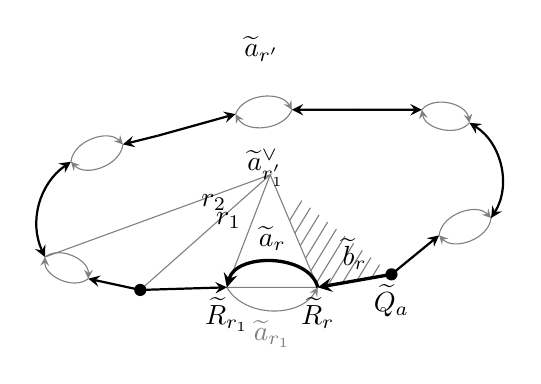
\begin{tikzpicture}[scale=1.1,>=stealth]
\coordinate (a) at (-3.0,0.4);\coordinate (b) at (-2.5,0.15);
\coordinate (c) at (-2.7,1.5);\coordinate (d) at (-2.1,1.7);
\coordinate (e) at (-0.8,2.05);\coordinate (f) at (-0.15,2.1);
\coordinate (g) at (1.35,2.1);\coordinate (h) at (1.9,1.95);
\coordinate (i) at (1.55,0.65);\coordinate (j) at (2.15,0.85);
\coordinate (k) at (-0.9,0.05);\coordinate (l) at (0.15,0.05);
\coordinate (q) at (1,0.2);\coordinate (u) at (-1.9,0.02);
\coordinate (o) at (-0.4,1.35);
\draw[gray] (a)--(o)--(u);\draw[gray] (o)--(l)--(k)--cycle;
\begin{scope}\clip (o)--(q)--(l)--cycle;
\foreach \x in {-0.8,-0.65,...,1.4}{\draw[gray] (\x,-0.2)--++(1.1,1.8);}\end{scope}
\draw[gray,->] (a) to[bend left=65] (b);\draw[gray,->] (b) to[bend left=65] (a);
\draw[gray,->] (c) to[bend left=65] (d);\draw[gray,->] (d) to[bend left=65] (c);
\draw[gray,->] (e) to[bend left=65] (f);\draw[gray,->] (f) to[bend left=65] (e);
\draw[gray,->] (g) to[bend left=65] (h);\draw[gray,->] (h) to[bend left=65] (g);
\draw[gray,->] (i) to[bend left=65] (j);\draw[gray,->] (j) to[bend left=65] (i);
\draw[very thick,->] (l) to[bend right=75] node[above] {$\widetilde a_r$} (k);
\draw[gray,->] (k) to[bend right=60] node[below] {$\widetilde a_{r_1}$} (l);
\draw[thick,<->] (a) to[bend left=40] (c);
\draw[thick,->] (-1.7,1.8)--(d);\draw[thick,->] (-1.7,1.8)--(e);
\draw[thick,->] (.6,2.1)--(f);\draw[thick,->] (.6,2.1)--(g);
\draw[thick,<->] (h) to[bend left=45] (j);
\draw[thick,->] (q)--(i);\draw[very thick,->] (q)--node[above] {$\widetilde b_r$}(l);
\draw[thick,->] (u)--(b);\draw[thick,->] (u)--(k);
\foreach \p in {u,q}{\fill (\p) circle (2pt);}
\node[below] at (k) {$\widetilde R_{r_1}$};\node[below] at (l) {$\widetilde R_r$};\node[below] at (q) {$\widetilde Q_a$};
\node[above] at (-.5,2.55) {$\widetilde a_{\unsure{r'}}$};
\node[below] at (-.45,1.75) {$\widetilde a_{\unsure{r'_1}}^{\unsure{\vee}}$};
\node at (-1.05,1.03) {$r_2$};\node at (-.88,.82) {$r_1$};
\end{tikzpicture}}

\[
\boxed{
\overbrace{\widetilde A_{\omega^n r''}\widetilde A_{\omega^{\unsure{m}}r''}\cdots\widetilde A_{r''}}^{\mu_{\widetilde Q_a}^{\omega}}
=\overbrace{\widetilde A_{\omega^n r_1}\widetilde A_{\omega^{n-1}r_1}\cdots\widetilde A_{r_1}}^{\mu_{\widetilde Q_{\unsure{i}}}^{\omega'}}}
\]
équivalent à ceci, \deleted{\unsure{bien que}}
\[
\deleted{\widetilde B'_{\omega^n r}\widetilde B_{\omega r}\cdots\widetilde B_{\unsure{r^*}}=\mu_r}
\]
\figure{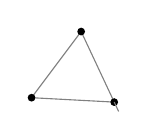
\begin{tikzpicture}[scale=.7]
\draw[gray] (0,0)--(.9,1.2)--(1.5,-.08)--cycle;
\fill (0,0) circle (2pt);\fill (.9,1.2) circle (2pt);\fill (1.5,-.08) circle (2pt);
\draw[gray] (1.5,-.08)--(1.58,-.25);
\end{tikzpicture}}

\scanpage{34}
\margin{33}
\unsure{UNIVERSITE} DES SCIENCES\\
ET\\
\unsure{TECHNIQUES} DU LANGUEDOC
\begin{flushright}- 5 -\end{flushright}
\begin{center}
PROPOSITIONS RELATIVES A L'AVANCEMENT POUR L'ANNEE 1980\\
MAITRES - ASSISTANTS
\end{center}
\diagram{
\begin{array}{|l|l|l|l|l|l|l|l|l|l|}
\hline
\begin{array}{l}\text{\unsure{Nom} et Ordre}\\\text{\unsure{de présentation}}\end{array} & \begin{array}{l}\text{Section}\\\text{C.C.U.}\end{array} & \begin{array}{l}\text{Date de}\\\text{naissance}\end{array} & \begin{array}{l}\text{Date d'entrée}\\\text{dans l'enseigne-}\\\text{ment}\\\text{supérieur}\end{array} & \begin{array}{l}\text{Classement}\\\text{actuel}\end{array} & \begin{array}{l}\text{Date dernière}\\\text{promotion}\\\text{d'échelon}\end{array} & \begin{array}{l}\text{Ancienneté}\\\text{au 1.01.1980}\\\text{}\\\text{(échelon)}\end{array} & \begin{array}{l}\text{Classe}\\\text{proposée}\end{array} & \text{Choix} & \text{Ancienneté}\\\hline
\text{GRANIER Willian} & \text{27e2e} & \text{29.12.44} & \text{1.10.64} & \text{1\textsuperscript{o} cl- 1\textsuperscript{o} ech} & \text{1.06.78} & \text{1 an 7m} & \text{1\textsuperscript{o}cl 2\textsuperscript{o}ech} & \text{1.12.80} & \text{}\\
\text{GUERIN Christian} & \text{27e1e} & \text{23.12.46} & \text{1.10.69} & \text{1\textsuperscript{o} cl- 1\textsuperscript{o} ech} & \begin{array}{l}\text{1.01.79}\\\text{avec 7m}\end{array} & \text{1 an 7m} & \text{1\textsuperscript{o}cl 2\textsuperscript{o}ech} & \text{1.12.80} & \text{}\\
\text{GUIDA Alain} & \text{27e} & \text{4.09.43} & \text{1.10.67} & \text{1\textsuperscript{o} cl- 1\textsuperscript{o} ech} & \begin{array}{l}\text{1.01.79}\\\text{anc. 2 ans}\end{array} & \text{3 ans} & \text{1\textsuperscript{o}cl 2\textsuperscript{o}ech} & \text{} & \text{1.01.80}\\
\text{HERBUTE Serge} & \text{31e} & \text{4.08.44} & \text{1.10.68} & \text{1\textsuperscript{o} cl- 1\textsuperscript{o} ech} & \begin{array}{l}\text{1.01.79}\\\text{avec 1 a 11m}\end{array} & \text{2 ans 11m} & \text{1\textsuperscript{o}cl 2\textsuperscript{o}ech} & \text{1.01.80} & \text{1.02.80}\\
\text{HOCQUEMILLER José} & \text{17e} & \text{3.11.35} & \text{1.10.59} & \text{1\textsuperscript{o} cl- 3\textsuperscript{o} ech} & \text{1.04.76} & \text{3 ans 9m} & \text{1\textsuperscript{o}cl 4\textsuperscript{o}ech} & \text{1.01.80} & \text{1.04.80}\\
\text{HOCQUEMILLER Marcel} & \text{17e} & \text{14.02.30} & \text{1.10.58} & \text{1\textsuperscript{o} cl- 4\textsuperscript{o} ech} & \begin{array}{l}\text{1.01.79}\\\text{avec 1a 9m}\end{array} & \text{2 ans 9m} & \text{1\textsuperscript{o}cl 5\textsuperscript{o}ech} & \text{1.01.80} & \text{1.04.80}\\
\text{ITIER Jean} & \text{27e} & \text{15.04.34} & \text{1.10.56} & \text{1\textsuperscript{o} cl- 5\textsuperscript{o} ech} & \text{1.01.77} & \text{3 ans} & \text{1\textsuperscript{o}cl 6\textsuperscript{o}ech} & \text{} & \text{1.01.80}\\
\text{JACQUEMIN J.Louis} & \text{23e} & \text{13.06.47} & \text{1.10.69} & \text{1\textsuperscript{o} cl- 1\textsuperscript{o} ech} & \text{1.02.78} & \text{1 an 11m} & \text{1\textsuperscript{o}cl 2\textsuperscript{o}ech} & \text{1.08.80} & \text{}\\
\text{JOULLIE André} & \text{21e} & \text{17.03.44} & \text{1.10.67} & \text{1\textsuperscript{o} cl- 1\textsuperscript{o} ech} & \text{1.11.77} & \text{2 ans 2m} & \text{1\textsuperscript{o}cl 2\textsuperscript{o}ech} & \text{1.05.80} & \text{1.11.80}\\
\text{Mme JOULLIE A.Marie} & \text{23e} & \text{10.10.43} & \text{1.10.68} & \text{1\textsuperscript{o} cl- 1\textsuperscript{o} ech} & \text{1.08.77} & \text{2 ans 5m} & \text{1\textsuperscript{o}cl 2\textsuperscript{o}ech} & \text{1.02.80} & \text{1.08.80}\\
\text{LABORDE Olivier} & \text{17e} & \text{6.12.45} & \text{1.10.68} & \text{1\textsuperscript{o} cl- 2\textsuperscript{o} ech} & \text{1.09.77} & \text{2 ans 4m} & \text{1\textsuperscript{o}cl 3\textsuperscript{o}ech} & \text{1.03.80} & \text{}\\
\text{LAVERGNE J.Pierre} & \text{27e} & \text{7.04.43} & \text{1.10.70} & \text{1\textsuperscript{o} cl- 1\textsuperscript{o} ech} & \text{1.01.78} & \text{2 ans} & \text{1\textsuperscript{o}cl 2\textsuperscript{o}ech} & \text{1.07.80} & \text{}\\
\text{LEGRAND Christiane} & \text{31e} & \text{5.11.35} & \text{1.10.59} & \text{1\textsuperscript{o} cl- 3\textsuperscript{o} ech} & \begin{array}{l}\text{1.10.80}\\\text{avec 2a 3m}\end{array} & \text{2 ans 3m} & \text{1\textsuperscript{o}cl 4\textsuperscript{o}ech} & \text{1.10.80} & \text{}\\
\text{LEMAIRE Catherine} & \text{18e} & \text{14.02.42} & \text{1.01.67} & \text{1\textsuperscript{o} cl- 2\textsuperscript{o} ech} & \begin{array}{l}\text{1.01.79}\\\text{avec 2a}\end{array} & \text{3 ans} & \text{1\textsuperscript{o}cl 3\textsuperscript{o}ech} & \text{1.01.80} & \text{}\\
\text{LEPETRE Thierry} & \text{21e} & \text{14.04.39} & \text{1.10.67} & \text{1\textsuperscript{o} cl- 2\textsuperscript{o} ech} & \begin{array}{l}\text{1.01.79}\\\text{avec 1a 14j}\end{array} & \text{2 ans 14j} & \text{1\textsuperscript{o}cl 3\textsuperscript{o}ech} & \text{17.06.80} & \text{}\\
\begin{array}{l}\text{Melle LEVALLOIS Christi-}\\\text{ne}\end{array} & \text{27e} & \text{8.09.36} & \text{15.10.60} & \text{1\textsuperscript{o} cl- 4\textsuperscript{o} ech} & \text{1.12.77} & \text{2 ans 1m} & \text{1\textsuperscript{o}cl 5\textsuperscript{o}ech} & \text{1.06.80} & \text{1.12.80}\\
\hline\end{array}}

\scanpage{36}
\margin{35}
\uline{Lemme} 1\quad soit $\overleftrightarrow{[x,y]}$ un segment

\deleted{\unsure{posons}}
\deleted{tel que la droite $\inserted{\Delta_0}$ de $\unsure{V}$ \unsure{orientée}}
\deleted{$\Delta$ une droite homogène qui ne}

orienté, ne contenant pas l'origine, d'où
\deleted{\unsure{contenant} $x,y$, on suppose que}
une orientation $\omega$ de $V$
\deleted{supposons que $x$ et}
(tel que l'orientation \inserted{de $\Delta_0$} induite par le
$\frac12$ plan contenant \deleted{$\unsure{\Delta}$} $0$
\deleted{\unsure{aille}} \inserted{soit} \deleted{\unsure{celle de}}
$x$ vers $y$).
\deleted{\unsure{On a de}} Soit
$\Delta$ une droite homogène \inserted{de $V$},
\deleted{\unsure{ne contenant pas}} \inserted{telle que}
\deleted{\unsure{passe à}} $\Delta\cap\{x,y\}=\varnothing$.
Considérons
\[
f_{x,y}(s,t)=(1-s)\varphi_\omega\Re l_{y,x}(t)+s\,l_{y,x}(t)
\]
qui, pour $t$ fixé, parcourt le segment joignant
$\varphi_\omega\Re l_{y,x}(t)$ à $l_{y,x}(t)$. Alors
$f_{x,y}([0,1]\times[0,1])$ ne rencontre pas $\Delta_{\mathbb C}$.

\margin{\unsure{Ceci ne marche pas pour} \unsure{un, pour voir ça}!}
\margin{$l_{y,x}(t)=\dfrac{x+y}{2}+e(t)\dfrac{x-y}{2}$\quad
$e(t)=\exp\unsure{2i\pi t}$.}

\uline{Corollaire}\quad \deleted{\unsure{On}.}
Si $x,y\in V^{**}$ \deleted{\unsure{on}} (et
(\deleted{$\unsure{x,y}$} $x,y$ non homothétiques i.e. $x,y$ correspondent
à des pts diff. de $\Sigma^*$) alors on a
commutativité dans $\Pi_1V^{**}$ :
\diagram{
\begin{tikzcd}[ampersand replacement=\&, row sep=large,column sep=huge]
x \arrow[r,"l_{y,x}"] \arrow[d,leftrightarrow,"{L_{\deleted{\unsure{y}},\unsure{x},\varphi_\omega(x)}}"'] \&
y \arrow[d,leftrightarrow,"{L_{y,\varphi_\omega(y)}}"] \\
\varphi_\omega(x) \arrow[r,"{\varphi_\omega(\deleted{\unsure{L}}l_{y,x})=L_{\varphi_\omega(y),\varphi_\omega(x)}}"'] \& \varphi_\omega(y)
\end{tikzcd}}
\margin{$L_{y,x}(t)=t(x-y)+y$}

\scanpage{37}
\margin{36}\margin{\textcircled{3}}
du Languedoc

\uline{Fonctionnement général de l'Université}
\[
\begin{array}{|l|r|r|r|r|r|}\hline
\text{DEPENSES}&1979&\text{DEPENSES }1979\ *&1980&+\ \text{POUR }1980&-\ \text{POUR }1980\\\hline
\text{Personnel}&114\ 000&123\ 841,28&135\ 000&21.000&-\\
\text{Charges}&38\ 500&36\ 000,00^*&40\ 000&1.500&-\\
\text{Impôts}&13\ 500&10\ 453,00^*&15\ 000&1.500&-\\
\text{Entretien mobilier}&7\ 500&3\ 274,57&10\ 000&2.500&-\\
\text{Ordinateur}&87\ 000&115\ 407,65&150\ 000&63.000&-\\
\text{Diffusions, papèterie}&119\ 000&63\ 657,47&71\ 500&-&47.500\\
\text{Petit matériel}&17\ 000&-&-&-&17.000\\
\text{Documentation}&15\ 000&10\ 971,28&15\ 000&-&-\\
\text{P.T.T.}&91\ 000&103\ 000,00&100\ 000&9.000&-\\
\text{Cellule informatique}&6\ 000&7\ 344,52&29\ 500&23.500&-\\
\text{Déplacements (compris commissions spéciales)}&75\ 000&75\ 000,00&78\ 000&3.000&-\\
\text{Publicité}&2\ 000&-&2\ 000&-&-\\
\begin{gathered}\text{Réception}\\\text{Arbre de Noël}\end{gathered}&\begin{gathered}50\ 000\\15\ 000\end{gathered}&\left\{36\ 463,32\right.&\left\{40\ 000\right.&&25.000\\
\begin{gathered}\text{\tikz[baseline=(a.base)]{\node[draw,ellipse,inner sep=1pt](a){Anglais};}}\\\text{Ass. Présidents}\end{gathered}&\begin{gathered}60\ 000\\4\ 500\end{gathered}&\left\{63\ 460,00\right.&\left\{\begin{gathered}-\\4\ 500\end{gathered}\right.&&\begin{gathered}60.000\\-\end{gathered}\\
\text{Subventions}&\underline{84\ 000}&\underline{84\ 000,00}&\underline{15\ 000}&-&\underline{69.000}\\
&799\ 000&732\ 853,09&705\ 500&\unsure{125.000}&218.500\\
\text{Intérêt emprunt}&16\ 000&15\ 955,44&-&-&16.000\\
\text{Remboursement emprunt}&228\ 000&227\ 935,25&-&-&228.000\\
\text{Gros matériel}&-&\left\{\begin{gathered}73\ 823,38\\8\ 225,19\end{gathered}\right.&37\ 128&\unsure{37.128}&-\\\cline{2-6}
&1\ 043\ 000&1\ 058\ 792,35^*&742.628&\unsure{162.128}&462.500\\\hline
\end{array}
\]
\margin{$\longleftarrow\boxed{\begin{gathered}\text{\unsure{Biol.}}\quad6500\\\text{\unsure{Hm.}}\quad6500\\\text{\unsure{Handi.}}\quad2000\end{gathered}}$}
* Exercice non terminé\par
évaluation.

\scanpage{38}
\margin{37}
\uline{Lemme 2} \inserted{(trivial)}
\deleted{On a} Posons, pour $x,y\in V$ et un chemin
$l:x\to y$ dans $V$
\[
g_{\deleted{\unsure{xy}}}(s,t)=\deleted{\unsure{1}}\ (1-s)\varphi_\omega l(t)+l(t)
\]
Soit $\Delta$ une droite de $V$ telle que
\deleted{$l[0,1]$} $|l|\cap\Delta=\varnothing$.
Alors $g([0,1]\times[0,1])\cap\Delta_{\mathbb C}=\varnothing$.
En effet, on a $\Re g([0,1]\times[0,1])=|l|$, et
$\Re\Delta_{\mathbb C}=\Delta$.

\uline{Corollaire}\quad \deleted{\unsure{On a Si on}} $l$ est un chemin
de $V^{**}$, on a commutativité de
\diagram{
\begin{tikzcd}[ampersand replacement=\&, row sep=large,column sep=huge]
\varphi_\omega(x) \arrow[r,"\varphi_\omega(l)"] \arrow[d,"{L_{x,\varphi_\omega(x)}}"'] \&
\varphi_\omega(y) \arrow[d,"{L_{y,\varphi_\omega(y)}}"]\\
x\arrow[r,"l"']\&y
\end{tikzcd}}

\uline{Lemme 3} \inserted{($\pm$ trivial)}
$|l_{y,x}|\cap\Delta_{\mathbb C}=\varnothing$ pour tte
droite $\Delta$ \inserted{(hom. ou non)} qui ne rencontre pas $\{x,y\}$.

Car comme $\Re l_{y,x}=[x,y]$,
on ne peut avoir $|l_{y,x}|\cap\Delta_{\mathbb C}\ne\varnothing$ que si
$\Delta\cap[x,y]\ne\varnothing$, donc (comme $\Delta\cap\{x,y\}=\varnothing$)
$\Delta\cap[x,y]=\{a\}$, $a\ne x,y$, \unsure{mais on aurait}
alors \deleted{$a=\unsure{x}$} $a=\Re l_{\unsure{x,y}}(t)$, avec $(t\ne0,1)$
$\operatorname{Im}l_{\unsure{x,y}}(t)=(\sin t)\dfrac{y-x}{2}$ donc
$y-x\in$ espace \deleted{\unsure{vect.}} des translations de $\Delta$
donc $x,y\in\Delta$\par
absurde

\scanpage{39}
\margin{38}\margin{\textcircled{2}}
\unsure{Université des Sciences et Techniques}\par du Languedoc

\uline{GRANDES MASSES DEPENSES}
\[
\begin{array}{|l|r|r|r|r|}\hline
\text{DEPENSES}&1979&1980&+\ \text{POUR }1980&-\ \text{POUR }1980\\\hline
\text{\unsure{Fonctionnement} général Université}\ \text{(voir3)}&799\ 000&705500&-&93.500\\
\text{\unsure{Matériel}}\quad\text{''}\quad\text{''}\quad\text{''}&-&37\ 128&37128&-\\
\text{\unsure{Remboursement} emprunt}&244\ 000&-&-&244000\\
\text{\unsure{Fonctionnement} général Campus}\ \text{(voir4)}&9\ 414\ 660&\unsure{9.075\ 900}&-&338760\\
\text{\unsure{Gros} travaux}&403\ 000&-&-&403000\\
\text{\unsure{Matériel}}&150\ 000&100000&-&50000\\
\text{\unsure{Bâtiment} Botanique}&343\ 726&340\ 000^*&-&3726\\
\text{\unsure{Station} de Sète}&40\ 000&40\ 000&-&-\\
\text{\unsure{UER}1 à4}\left\{\begin{gathered}\text{Fonctionnement}\\\text{Matériel}\end{gathered}\right.&\begin{gathered}1\ 627\ 131\\163\ 829\ \checkmark\end{gathered}&\begin{gathered}1\ 627\ 131\\{}[163\ 829\end{gathered}&\begin{gathered}-\\-\end{gathered}&\begin{gathered}-\\-\end{gathered}\\
\text{\unsure{C.P.A.}}&29\ 040&29\ 040&-&-\\
\text{\unsure{UER}5 à9 Fonctionnement}&7\ 500&7\ 500&-&-\\
\text{\unsure{Moniteurs}6 mois (82)}&409\ 952&182\ 122&-&227830\\
\text{\unsure{A} + Réserve}&200\ 000&215000&15000&\\
\text{\unsure{3} mois moniteurs (82)}&206\ 090&91\ 061\ \dashv&-&115029\\
\text{\unsure{Matériel}}&&&&\\
\text{\illegible{1}}&-&-&-&-\\\cline{2-5}
\text{TOTAL :}&14\ 037\ 928&\unsure{12.614.211|13.614.211}&52.128&1.475.845\\\hline
\end{array}
\]
\unsure{*} Evaluation\par
\unsure{Les} taxes d'apprentissage ne sont pas prises en compte ISI $\unsure{\#}$ $332\ 000$\par
\hfill Autres $\unsure{\#}$ $170\ 000$

\margin{$\begin{gathered}\text{Subvention matériel}\\750.957\end{gathered}\left\{\begin{array}{lr}
\text{F. G\textsuperscript{al} Univ.}&\unsure{37.128}\\
\text{'' Campus}&100000\\
\text{1 à4}&163.829\\
\text{5 à9}&450.000
\end{array}\right.$}

\scanpage{40}
\margin{39}
\uline{Lemme 4}\quad Posons
$l_x(t)=l_{-x,x}(t)=e(t)x:x\to\unsure{-x|x}$
et considérons
\[
\begin{aligned}
h(s,t)&=(1-s)\deleted{\unsure{\varphi_\omega(\Re l_x(t))}}l_{\varphi(x)}(t)+s\,l_x(t)\\
&=e(t)\bigl((1-s)\varphi(x)+sx\bigr)
\end{aligned}
\]
Alors pour tte droite hom. $\Delta$ de $V$
\deleted{que} telle que $x\notin\Delta$, on a
\[
h([0,1]\times[0,1])\cap\Delta_{\mathbb C}=\varnothing
\]
En effet, $h(s,t)\in\Delta_{\mathbb C}\Longleftrightarrow
(1-s)\varphi(x)+sx\in\Delta_{\mathbb C}$
\[
\underset{\text{\unsure{passer à} }\Re}{\Longrightarrow}
(1-s)x+sx\in\Delta\qquad\text{i.e. }x\in\Delta
\]

\uline{Corollaire}\quad On a commutativité dans
$\Pi_1V^{**}$, si $\unsure{x}\in V^{**}$ :
\diagram{
\begin{tikzcd}[ampersand replacement=\&, row sep=large,column sep=huge]
\varphi_\omega(x)\arrow[r,"l_{\varphi_\omega(x)}"]\arrow[d,"{L_{x,\varphi_\omega(x)}}"']\&-\varphi_\omega(x)\arrow[d,"{L_{-x,\unsure{-\varphi_\omega(x)|\varphi_\omega(x)}}}"]\\
x\arrow[r,"l_x"']\&-x
\end{tikzcd}}

\scanpage{41}
\margin{40}
17--1\qquad Arnaud BEAUVILLE (Angers)\par
François DRESS (Bordeaux)\par
Daniel FERRAND (Rennes)\par
Jean Marc FONTAINE (Grenoble)\par
Jean GIRAUD (Orsay)\par
Georges GRAS (Besançon)\par
Serge GRIGORIEFF (Lyon)

Gérard RAUCH (Mulhouse)\par
Michel RAYNAUD (Orsay)\par
Jacques STERN (Caen)\par
Michel WALDSCHMIDT (Paris 6)

17--2\qquad Marc AUTHIER (Reims)

Louis BOUTET DE MONVEL (Paris 6)\par
Jacques CARMONA (Marseille-Luminy)\par
Jacques CHAZARAIN (Nice)

Michel DUFLO (Paris 7)

Jacques FARAUT (Strasbourg)\par
Jean-Pierre FERRIER (Nancy)

Francis SERGERAERT (Poitiers)

17--3\qquad Daniel BERNARD (Strasbourg)\par
Yves COLIN DE VERDIERES (Grenoble)\par
André GRAMAIN (Tours)

Jean Michel LEMAIRE (Nice)\par
Robert MOUSSU (Dijon)\par
Joseph LE POTIER (Paris 7)\par
Jean PRADINES (Toulouse)

\scanpage{43}
\margin{42}
Soient $n$ un entier $\ge3$, et considérons un
polygône régulier à \inserted{$m=$} $2n$ côtés, dans un
espace vectoriel \inserted{réel} $V$ de dimension 2.
L'ens des sommets $\widetilde{\unsure{I|J}}$ du polygone forme
\inserted{l'ens des sommets d'}un
polygône combinatoire (on dira aussi qu'il est muni d'une structure de polygone
combinatoire, exprimable de diverses façons équivalentes bien connues), dont
la donnée équivaut, à isom. can. près, à celle du plan vectoriel réel $V$
et du polygône régulier dans $V$. La donnée de l'un ou de l'autre
équivaut en effet à celle d'un torseur sous le groupe diédral
\[
(1)\qquad D_m=\mu_m\,\unsure{\rtimes|\cdot}\,\mathbb Z/2\mathbb Z
\]
\margin{(produit $\frac12$ direct, $\mathbb Z/2\mathbb Z$ opérant sur $\mu_m$ via
$\zeta\mapsto\zeta^{-1}$)}
qui est le groupe d'automorphismes de la structure standard
\[
(2)\qquad V_0=\mathbb C,\quad
\widetilde{\unsure{I|J}}_0=\mu_m\overset{\mathrm{def}}={}_m\mathbb C^*\subset V_0
\]
$\mu_m$ opérant sur $(V_0,\widetilde{\unsure{I|J}}_0)$ par homothéties
\[
z\longmapsto\zeta z\qquad(\zeta\in\mu_m)
\]
et $\mathbb Z/2\mathbb Z$ par conjugaison complexe
$z\longmapsto\overline z$

\margin{il suffirait $n\ge2$, mais le cas $n=2$ \unsure{est un cas}
très dégénéré, \unsure{qui ne présente pas certaines particularités combinatoires},
\unsure{manque bien} d'intérêt, \unsure{car} c'est le cas \unsure{de} d'un trou!}

\scanpage{44}
\margin{43}
On posera
\[
(3)\qquad D=D_{\widetilde{\unsure{I|J}}}=\operatorname{Aut}(V,\widetilde{\unsure{I|J}}).
\]
\[
(4)\qquad\underline\omega=\underline\omega_{\widetilde{\unsure{I|J}}}
=\Omega(\widetilde{\unsure{I|J}})\simeq\Omega^{\unsure{\vee}}(V)
\]
\margin{ens des orientations du poly. comb. $\widetilde{\unsure{I|J}}$,
ou de l'espace vectoriel réel $V$}

On a dans $D$ le sous-groupe $D^+$ des rotations, qui est le noyau
de l'hom naturel \inserted{(transp. de str.)}
$D\longrightarrow\mathbb Z/2\mathbb Z\simeq\operatorname{Aut}(\omega)$,
d'où suite exacte
\diagram{ (5)\quad\begin{tikzcd}[ampersand replacement=\&, column sep=large]
1\arrow[r,dash]\&D^+\arrow[r]\&D\arrow[r]\&\mathbb Z/2\mathbb Z\arrow[r,dash]\&1
\end{tikzcd}}
$\mathbb Z/2\mathbb Z$ opérant sur $D^+$ par $\zeta\mapsto\zeta^{-1}$.
On \deleted{y a un point} \inserted{a un plongement}
\[
(6)\qquad\omega\subset D^+
\]
et $\underline\omega$ est formé de deux rotations inverses l'une de l'autre,
d'angle $\dfrac{2\pi}{m}$ \deleted{pour l'} \inserted{dans le} sens de
\deleted{l'} \inserted{l'une et l'autre} orientations du $V$.
Ce sont deux générateurs de $D^+$, inverses
\deleted{\unsure{de l'un}\ \unsure{On si}}
\inserted{l'un de l'autre $\omega'=\omega^{-1}$,}
\inserted{le choix de $\omega$ \unsure{impliquant} un iso canonique}
\margin{$\mathbb Z/m\mathbb Z\overset\sim\longrightarrow D^+$}
Les \deleted{points de} sommets du polygône seront désignés indifféremment par
$\widetilde R_i$ $(i\in\widetilde{\unsure{I|J}})$.
On n'a pas utilisé encore le fait que $m$ est pair, ce qui équivaut au fait que
l'ens des $\widetilde R_i$ dans $V$ est stable par la symétrie
$x\mapsto\deleted{\unsure{+}}-x$

\scanpage{45}
\mspage{2}\margin{44}
\deleted{donc} \inserted{ou encore,} qu'on a un élément
\deleted{privilégié \unsure{d'ordre}} \inserted{d'ordre 2}
\[
(7)\qquad a_0\deleted{\unsure{a}}\in D^+
\qquad a_0:x\longmapsto-x
\]
qui est en fait le seul élément \inserted{d'ordre 2} $D^+$.
Si à tout $j\in\widetilde{\unsure{I|J}}$ on associe l'unique
\deleted{\unsure{réflexe}} élément $r_j\in D$ (une réflexion)
\deleted{donc} qui soit $\ne1$ et telle que
\[
(8)\qquad r_j(\widetilde R_j)=\widetilde R_j
\]
on aura
\[
(9)\qquad r_j=r_{a_0(j)},
\]
\deleted{et} donc il n'y a que $n=m/2$ réflexions $r_j$ distinctes,
qui correspondent à la moitié des éléments de la classe \inserted{non neutre}
$D^-$ de $D$ modulo $D^+$. Les autres réflexions sont celles associées aux
\uline{côtés} du polygone envisagé.

Il y a sur $V$ une unique forme quadratique invariante par $D$
(ou seulement par $D^+$), et égale à 1 sur les $\widetilde R_j$.
On considère $V$ comme espace \inserted{vect.} euclidien, grâce à cette forme.

\margin{\uline{NB} \deleted{$\unsure{a_0}$} \inserted{\unsure{Le centre} de}
$D$ est réduit à $\{1,a_0\}$, $m$ pair signifie \unsure{donc que}
le centre de $D$ est $\ne\{1\}$.}
\margin{\deleted{$\unsure{a_0}$ \illegible{2} \unsure{qui fixe}
$\unsure{aR}$ \unsure{des vecteurs positifs}} \deleted{\unsure{point}}
d'ordre 2}

\scanpage{46}
\margin{45}
\figure{
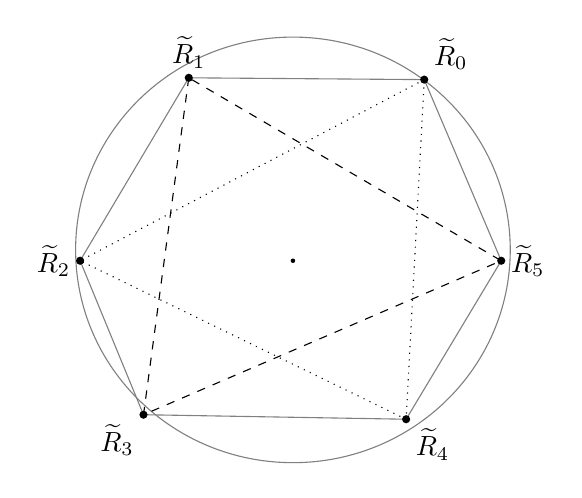
\begin{tikzpicture}[scale=1.15]
\coordinate (r0) at (1.35,2);\coordinate (r1) at (-1.25,2.02);
\coordinate (r2) at (-2.45,0);\coordinate (r3) at (-1.75,-1.7);
\coordinate (r4) at (1.15,-1.75);\coordinate (r5) at (2.2,0);
\draw[gray] (-.1,.12) ellipse (2.4 and 2.35);
\draw[gray] (r0)--(r1)--(r2)--(r3)--(r4)--(r5)--cycle;
\draw[dotted] (r0)--(r2)--(r4)--cycle;
\draw[dashed] (r1)--(r3)--(r5)--cycle;
\fill (-.1,0) circle(.025);
\foreach \p in {r0,r1,r2,r3,r4,r5}{\fill (\p) circle(.045);}
\node[above right] at(r0){$\widetilde R_0$};\node[above] at(r1){$\widetilde R_1$};
\node[left] at(r2){$\widetilde R_2$};\node[below left] at(r3){$\widetilde R_3$};
\node[below right] at(r4){$\widetilde R_4$};\node[right] at(r5){$\widetilde R_5$};
\end{tikzpicture}}
On s'intéresse au \unsure{complexifié} $V_{\mathbb C}$, et à la droite
projective complexe
\deleted{$\Sigma_{\widetilde{\unsure{I|J}}}=$}
\[
(10)\qquad\Sigma_{\widetilde{\unsure{I|J}}}(\mathbb C)
=\Sigma_{\widetilde{\unsure{I|J}}}=\Sigma
=\mathbb P(V_{\mathbb C})
=V_{\mathbb C}^*/\mathbb C^*,
\]
\deleted{les} sur laquelle $D$ opère, le noyau de cette opération étant le centre
$\{1,a_0\}$ i.e. $D$ opère par l'intermédiaire de
\[
(11)\qquad D'=D/\{1,a_0\}
\]
(isom. au groupe diédral $D_n$). On désigne par $R_i\in\Sigma$
l'image de $\widetilde R_i$ dans $\Sigma$, de sorte qu'on aura
\[
(12)\qquad R_i=R_{a_0(i)},
\]
En fait l'ens des $R_i$ est indexé de façon naturelle par l'ens quotient
\[
(13)\qquad\unsure{I|J}=\widetilde{\unsure{I|J}}/\{1,a_0\}.
\]

\margin{\uline{NB} $(\Sigma,\unsure{I|J}\subset\Sigma)$ étant donnés
($\Sigma$ comme droite projective complexe, ou comme sphère conforme orientée\ldots)
on a \unsure{équivalemment} un torseur sous $D_n$ $(\ne D_m!)$
\unsure{étant donné}, on peut en déduire $(V,\widetilde{\unsure{I|J}})$
à isom \unsure{non can.} près (i.e. un torseur sous $D_m$), mais seulement
modulo twist par $\{\pm1\}$-torseur\ldots On peut lever l'ambiguïté en imposant
une structure suppl. sur $\widetilde{\unsure{I|J}}$, à savoir la donnée
d'un élément de $\widetilde{\unsure{I|J}}/(D^+)^2$ i.e. de l'un
des deux $n$-gônes dans le $2n$-gône $\widetilde{\unsure{I|J}}$
\unsure{est stable par} $\unsure{C}$ \unsure{pour les ``positifs''}\ldots}

\scanpage{47}
\mspage{3}

L’ens des points fixes de $D'$ opérant sur
$\Sigma$ est \deleted{\unsure{indexé}} réduit à deux éléments,
un dans chacun des deux hémisphères
en lesquels $\Sigma_{\mathbb R}=P(V)$ découpe $\Sigma$ —
on a :
\[
(14)\qquad \pi_0(\Sigma\setminus\Sigma_{\mathbb R})\simeq
\begin{gathered}\underline\omega\\[-.5ex]\Vert\\[-.5ex]\Omega(\Sigma_{\mathbb R})\end{gathered}
\]
\margin{conv. de Stokes, provenant de l’orientation can. de $\Sigma$)}

donc les deux “pôles” seront indexés par
$\underline\omega$, et notés $\unsure{P|R}_\omega$
\[
(15)\qquad\left\{
\begin{aligned}
&P_\omega\qquad(\omega\in\underline\omega)\\
&P_\omega=\underbrace{\Sigma^{D^+}}_{\substack{\text{inv. sous}\\D^+\text{ op.}\\\text{sur }\Sigma}}
\cap\underbrace{\Sigma_\omega}_{\substack{\text{comp. conn.}\\\text{de }\Sigma\setminus\Sigma_{\mathbb R}\text{ indexée}\\\text{par }\omega}}
\end{aligned}\right.
\]

Si on exprime la définition de $\Sigma^{D^+}$ en
termes d’algèbre linéaire, on trouve que
ce sont les \uline{droites} \inserted{\uline{propres}} dans $V_{\mathbb C}$
\deleted{propres} \inserted{pour}
l’action de $D^+$. Mais considérons
la \unsure{double|seule} structure euclidienne sur $V_{\unsure{\mathbb C|\mathbb R}}$,
qui \deleted{\unsure{définit}} s’étend en une structure

\margin{46}

\scanpage{48}
quadratique non dégénérée sur $V_{\mathbb C}$,
\unsure{pour|par} laquelle $V_{\mathbb C}$ se décompose en
sous espaces isotropes
\[
(16)\qquad V_{\mathbb C}=\bigoplus_{\omega\in\underline\omega}V_{\mathbb C}^{\omega}
\]
qui sont aussi les sous-espaces propres
pour le groupe \inserted{$O^+(V)$} des rotations de $V$.
La donnée d’une orientation \inserted{$\omega$} de $V$
permet de définir un autom \unsure{d}
\[
(17)\qquad\left\{\begin{aligned}
&u_\omega\in\deleted{\unsure{\operatorname{Aut}}_{\mathbb R}(V)}\ O^+(V)\\
&u_\omega^2=-1
\end{aligned}\right.
\]
\margin{rotation d’un quart de tour dans le sens de l’orientation $\omega$}
d’où une structure complexe sur
$V$\inserted{(qui devient un \unsure{vect.} complexe de rang $1$, soit $V_{(\omega)}$)}, en faisant opérer $i\in\mathbb C$ par
\[
i\mathbin{\underset{\omega}{\cdot}}x=u_\omega x
\]
Mais par la définition universelle du
complexifié, la \deleted{structure} application
$\mathbb R$-linéaire $V\longrightarrow V_\omega$ se prolonge
canoniquement en une application

\margin{47}

\scanpage{49}
\mspage{4}

$\mathbb C$-linéaire, \deleted{\unsure{commutant} d’ailleurs (par tr. de str.)}
\[
(17')\qquad V_{\mathbb C}\xrightarrow{p_\omega}V_{(\omega)}
\]
\margin{cette application commute par transport de str. \unsure{à|:}
$O^+(V)$ (opérant sur $V_{\mathbb C}$ par complexification}

d’où une application \inserted{$\mathbb C$-lin.} canonique
$V_{\mathbb C}\longrightarrow\prod_{\omega\in\underline\omega}V_{(\omega)}$,
qui est un isomorphisme
\[
(18)\qquad p=(p_\omega)_{\omega\in\underline\omega}:
V_{\mathbb C}\xrightarrow{\sim}\prod_{\omega\in\underline\omega}
\underbrace{V_{(\omega)}}_{\simeq V_{\mathbb C}^{\omega}}.
\]
\margin{l’opération d’homothétie $i$ sur $V_{\mathbb C}$
\deleted{\unsure{comme}} \inserted{\unsure{s’identifie}}
\unsure{au prod des} $u_\omega$ sur les facteurs $V_{(\omega)}$}

Les $V_{\omega}$ sont apparus comme
des quotients de $V_{\mathbb C}$, si on veut les
regarder comme sous-espaces\inserted{— \unsure{auquel|auxquels} corresp. la \unsure{not°} $V_{\mathbb C}^{\omega}$ —} on trouve
que
\[
\begin{aligned}
(19)\qquad V_{\mathbb C}^{\omega\deleted{\unsure{\mathbb C}}}
&=\operatorname{Ker}\bigl(V_{\mathbb C}\xrightarrow{p_{\omega'}}V_{(\omega')}\bigr)\\
&=\{x\in V_{\mathbb C}\mid u_{\omega_{\mathbb C}}(x)=i.x\}
\end{aligned}
\]
\margin{\uline{\unsure{Ainsi|Aussi}}
$V_{\mathbb C}^{\omega}=\{\underbrace{x\unsure{-|+}iu_\omega x}_{\substack{\Vert\\\varphi_\omega(x)}}\mid x\in V\}$,
\unsure{où} $\varphi_\omega:V\xrightarrow{\sim}V_{\mathbb C}^{\omega}$
le $\mathbb R$-isom. inverse de $p_\omega$ $(17')$}

En fait, les $V_{\mathbb C}^{\omega}$\inserted{$(\omega\in\underline\omega)$} sont des sous-espaces
propres pour l’action de $O^+(V)$, i.e.
stables pour cette action, tandis que
les éléments de $O^-(V)$ les interchan-
gent.
\margin{vérifier que cette indexation des sous-espaces propres
$V_{\mathbb C}^{\omega}$ coïncide avec celle définie par la conv. de Stokes}

On s’intéresse au fibré vectoriel

\margin{48}

\scanpage{50}
$\mathcal O_{\unsure{\underline\Sigma|\Sigma}}(1)$ sur $\Sigma$, défini par la représentation (10) de $\Sigma$ comme \deleted{fibré} \unsure{espace} projectif associé à un vectoriel bien déterminé.

Je désigne par $P\Sigma_{J,\mathbb C}$ ou simplement $P\Sigma$ le fibré principal associé de groupe $\mathbb C^*$ (en des espaces analytiques complexes, disons, avec sa topologie habituelle --- pour le moment on ne travaille pas dans le contexte des schémas\ldots). \deleted{\unsure{I}}

Un point $x$ de $\Sigma$ étant une droite $F$ de $V$ \deleted{\unsure{de $D$}}, on a des isom. can.
\[
(18)\qquad
\left\{\begin{aligned}
\unsure{\check V|\mathbb V}(\underline{\mathcal O}(1))_x&=\deleted{\unsure{\Delta}}V/F\\
F\otimes\mathcal O_F(1)&\simeq\det(V)\simeq\mathbb R(\underline\omega)\left(\overset{\mathrm{déf}}=\mathbb R\mathbin{\wedge}_{\{\pm1\}}\underline\omega\right)\\
\mathcal O_F(1)&\simeq\check F(\omega)\left(\overset{\mathrm{déf}}=\check F\mathbin{\wedge}_{\{\pm1\}}\underline\omega\right)\simeq F^\perp
\end{aligned}\right.
\]
\inserted{$\mathcal O_F(1)\overset{\mathrm{déf}}=$}
\margin{d'où pass. à dét}
\margin{\unsure{i.e.}}
\deleted{\unsure{$\mathbb R\otimes$}}
\margin{orth. pour la str. quadratique \unsure{invariante\ldots}}

d'où
\[
(19)\qquad(P\Sigma)_x=(P\Sigma)_F\simeq(V/F)^*\simeq(\check F)^*\mathbin{\wedge}_{\{\pm1\}}\underline\omega\simeq F^\perp
\]
\deleted{et par un} isom.\unsure{$^s$} compatibles avec l'action de $\mathbb C^*$ (opérant sur $\check F$ par contragrédience de son action sur $F$), on aura
\[
\deleted{\unsure{(19)}}\quad(20)\qquad(P\Sigma)_x\simeq F^*\mathbin{\wedge}_{\{\pm1\}}\underline\omega=(F\mathbin{\wedge}_{\{\pm1\}}\underline\omega)^*\simeq(F^\perp)^*
\]
\mspage{49}

\scanpage{51}
\mspage{5}
en notant que pour deux droites vectorielles en dualité $F,F'$, on a $F^*\simeq F'^*$ can., --- mais cet isom. (20) \deleted{\unsure{doit}} \uline{renverse} l'\uline{action} de $\mathbb C^*$.
\inserted{de $(P\Sigma)_x$ et $(F\mathbin\wedge\omega)^*$}

On trouve ainsi des iso
\[
(21)\quad\left\{\begin{aligned}P\Sigma&\simeq(V(\omega))^*\\P\Sigma&\simeq V^*\end{aligned}\right.
\]
\diagram{\begin{tikzcd}[ampersand replacement=\&, column sep=small]
\deleted{\unsure{F}}\otimes\deleted{\unsure{F'}}\arrow[r] \&\deleted{\unsure{D}}\arrow[r]\&\deleted{\unsure{\mathbb C}}\\
\deleted{\unsure{F/e}}\&\&
\end{tikzcd}}
\margin{qui transforme le couple $(x,e\in(P\Sigma)_x\simeq\check F(\omega)\simeq F^\perp)$ \unsure{en} $F(\omega)^*\subset V(\omega)^*$ ; soit en $\check e$, considéré comme élém\unsure{$^t$} de $(F^\perp)^*\subset V^*$ soit en $e$, considéré comme élém\unsure{$^t$} de $\mathbb C^*$. Ces iso (21) \unsure{sont compatibles} à l'action de $D$ (\unsure{le groupe de structure}).}

Mais on a un isom canonique (provenant du produit extérieur
\[
V\simeq\check V(\omega)\qquad\deleted{et}
\]
et un isom canonique (provenant de la forme quadratique
\[
V\longrightarrow\check V\qquad\text{donc}\qquad\check V(\omega)\simeq V(\omega)
\]
d'où un isom canonique
\[
(21)\qquad V\xrightarrow{\sim}V(\omega)
\]
qui explicite le passage de l'un à l'autre isom. \deleted{\unsure{commutant d'ailleurs aux actions de $\mathbb C^*$}} (21). D'ailleurs, (21) induit \deleted{$D$, et par \unsure{transposant} l'identité} un isom
\diagram{\begin{tikzcd}[ampersand replacement=\&]
\deleted{\Sigma\simeq P(V)}\arrow[r,"\deleted{\mathrm{id}}"]\&\deleted{\Sigma\simeq P(V(\omega))}
\end{tikzcd}}
\diagram{\begin{tikzcd}[ampersand replacement=\&]
\text{(22)}\quad\Sigma=P(V)\arrow[r,"\sigma"]\&P(V(\omega))\quad(\deleted{\unsure{\Sigma}}\simeq\Sigma=P(V))
\end{tikzcd}}
(\deleted{qui est} la \deleted{\unsure{rotat\textsuperscript{n}}} symétrie p.r. à l'axe polaire, \inserted{qui du point de vue linéaire s'exprime} \deleted{i.e. l'\unsure{échange} de} comme le passage de $F$ à $F^\perp$). \deleted{et}

\deleted{par cet iso., \unsure{\illegible{1}} à $F$ correspond : $F'(\omega)(\simeq F^\perp)$ dans $V(\omega)$ \unsure{avec} \inserted{(où $F'\subset V$, en fait $F'=F^\perp$)} \unsure{on a} $F\longmapsto F'(\omega)$ i.e. $F(\omega)\simeq F'$.}
\mspage{50}

\scanpage{52}
Je travaillerai \deleted{donc} avec l'iso.
\[
(23)\qquad P\Sigma\simeq V^*
\]
plutôt qu'avec $P\Sigma\simeq V(\underline\omega)^*$, \deleted{\unsure{ce qui}} qui respecte l'action de $\mathbb C^*$ \deleted{\unsure{\illegible{1}}} (au lieu de la remplacer par l'action inverse), mais qui, par contre, n'est pas compatible aux projections --- on a seulement \unsure{d'int.}
\diagram{\begin{tikzcd}[ampersand replacement=\&, row sep=large,column sep=large]
P\Sigma_{\unsure{\Sigma}}\arrow[r,"\sim","(23)"']\arrow[d,"{\mathrm{proj.can.}}"']\&V^*\arrow[d,"{\mathrm{proj.can.}}"]\\
\Sigma\arrow[r,"\sigma"]\&\Sigma\simeq V^*/\mathbb R^*
\end{tikzcd}}
\margin{(24)}

\margin{Toute la digression précédente est un pur ``\unsure{sexe des anges}''. À retenir : pour le fibré vectoriel \deleted{\unsure{F}} \unsure{intrinsèque} $\underline L$ \deleted{\unsure{pour}} sur $\Sigma$ (\unsure{au moins dans le cas $n=3$}) au dessus d'un point $R_i\in\Sigma$, il y a un point $\widetilde R_i$ canonique (\unsure{impliquant des choix} \deleted{\unsure{amples}} \unsure{identifiés à} un $\omega\in\underline\omega$), et qui \deleted{$\unsure{\Gamma(\Sigma,L)}$} \deleted{$\unsure{\Gamma(\Sigma,L)}$} \unsure{identifie les} $\check R_i$ à des éléments de $\Gamma(\Sigma,\underline L)(\omega)\overset{\mathrm{déf}}=\check V$, dont la somme est $0$, et qui engendrent, \unsure{d'où un isom} $V\simeq\mathcal O^J/\mathcal O$ (diagonale) \unsure{--- le tout} \unsure{avec les flèches} \deleted{\unsure{et $\omega\in$}} \uline{\unsure{sur $\Sigma$}}. Ceci \unsure{se relativise} sur $\mathbb Z$. $\Sigma$ : un \deleted{\unsure{$V^*/\mathbb C^*$}} $V^*/\mathbb C^*$, \unsure{désigne par} $\check V$, $P\Sigma$ \unsure{``précisément comme les droites de la droite $L_x$''}, \uline{avant} de l'opération des $\mathbb C^*$) et \unsure{n'y a pas} dans $V=\Gamma(\Sigma,\underline L)(\omega)$ \unsure{qu'il faut prendre} (\unsure{plutôt} $V=\operatorname{Ker}(\mathcal O^J\to\mathcal O)$), $V=\mathcal O^J/\mathcal O$. Cet \uline{iso} est bien précis sur les \unsure{3 isom}, on a \unsure{une} commut\unsure{$^{\mathrm{n}}$} à l'action de $D\,(\simeq\unsure{\mathfrak S_3})$.}

Notons en passant que si $\tau$ désigne la conjugaison complexe (de $V_{\mathbb C}$ ou $\Sigma$) on aura
\[
(25)\qquad\tau\deleted{\unsure{\circ}}\sigma=\underline a\quad\text{ou ``antipodisme'' de }\Sigma\quad\ldots
\]
Je m'intéresse à l'ouvert
\[
(26)\qquad\Sigma^*=\Sigma-\{R_i\mid i\in J\}
\]
et à : \deleted{\unsure{B}}
\[
(27)\qquad P\Sigma^*=P\Sigma\mid\Sigma^*\overset{(23)}\simeq V^{**}=V-\bigcup_{i\in J}\Delta_i
\]
où les $\Delta_i$ sont les $n=m/2$ \uline{diagonales} du
\mspage{51}

\scanpage{53}
\mspage{6}
polygone régulier. Je veux décrire des groupoïdes équivalents aux groupoïdes fondamentaux
\[
(28)\qquad\Pi_1P\Sigma^*\simeq\Pi_1V^{**},\qquad\Pi_1\Sigma^*
\]
par générateurs et relations, avec des sommets bien choisis dans les espaces envisagés, stables par l'action de $D$ ainsi que de celle de $\tau$. Bien sûr, il faut garder présent le morphisme de groupoïdes
\diagram{\begin{tikzcd}[ampersand replacement=\&]
\text{(29)}\quad\Pi_1P\Sigma^*=\Pi_1V^{**}\arrow[r,no head]\&\Pi_1\Sigma^*
\end{tikzcd}}
Sur la situation (28), (29) opère le groupe
\[
\deleted{\unsure{\mathbb C}}\quad D\times\mathbb C^*\times\{1,\tau\}
\]
\margin{$D$ opère tautologiquement $\mathbb C^*$ par homothéties (mais c'est l'action \uline{opposée} de celle dans $P\Sigma^*$)}
\margin{\uline{NB} $\sigma$ n'opère sur $\Sigma^*,P\Sigma^*$ que si $n$ est pair (donc \inserted{pas dans le cas $n=3$} le plus \deleted{\unsure{intéressant}}).}
\margin{\uline{NB} action des groupes \uline{compatibles}, l'élément $(\unsure{\sigma_0},-1)$ opère trivialement}
on s'intéresse à l'action du sous-groupe fini
\[
(30)\qquad D\times\mu_m\times\{1,\tau\}
\]
\margin{d'ordre \deleted{\unsure{4}} $4m^2=16n^2$ ($144$ si $n=3$) mais \unsure{qui en fait a le quotient} fidèle est d'ordre $8n^2$ ($72$ si $n=3$)}
\margin{\uline{NB}. c'est le quotient $(D\times\mu_m)/\{\pm1\}\times\{1,\tau\}$ qui opère fidèlement.}
On peut \unsure{d'ailleurs} prendre le sous-groupe
\[
(31)\qquad D^+\times\mu_m\simeq\mu_m(\underline\omega)\times\mu_m
\]
de (30), en notant que pour la représentation
\mspage{52}

\scanpage{54}
(\unsure{16}) (18), $V_{\mathbb C}\simeq\bigoplus_{\omega\in\underline\omega}V_{\mathbb C}^{\omega}$, le groupe produit $\mu_m^{\underline\omega}$ d'ordre $m^2$ opère sur $V_{\mathbb C}$, par
\[
(32)\qquad(\lambda_\omega)_{\omega\in\underline\omega}\cdot(x_\omega)_{\omega\in\underline\omega}=(\lambda_\omega x_\omega)
\]
On \deleted{\unsure{va}} a des hom
\[
(33)\qquad\left\{\begin{aligned}
\mu_m&\longrightarrow\mu_m^{\underline\omega}\qquad\text{hom diagonal}\\
\mu_m(\omega)\simeq D^+&\longrightarrow\mu_m^{\underline\omega}\\
\lambda&\longmapsto(\unsure{\lambda^\omega|\lambda_\omega})_{\omega\in\underline\omega}\quad\deleted{\unsure{\mathrm{dont}}}
\end{aligned}\right.
\]
tels que les actions de $\mu_m,D^+$ sur $V^{\deleted{\unsure{\omega}}}$ \deleted{\unsure{passent}} passent via celle de $\mu_m^{\underline\omega}$. L'hom correspondant
\[
(34)\qquad\deleted{\unsure{\mu_m}}\underset{\mu_m(\underline\omega)}{\underbrace{D^+}}\times\mu_m\longrightarrow\mu_m^{\underline\omega}
\]
entre groupes de $=$ ordre $m^2=4n^2$ a comme noyau le sous-groupe d'ordre $2$ engendré par \deleted{$\unsure{a_0,-1}$} $(a_0,-1)$, son image est donc d'indice $2$, elle est formée des couples $(\lambda_\omega)_{\omega\in\underline\omega}$ tels que l'on ait
\[
(35)\qquad\deleted{\unsure{\prod\lambda_\omega}}\left(\prod_{\omega\in\underline\omega}\lambda_\omega\right)^n=1\qquad\mathrm{i.e.}\quad(\lambda_\omega\lambda_{\omega'})^n=1.
\]
Notons que les autom. de $V_{\mathbb C}$ qui stabilisent $V_{\mathbb C}^{**}$ i.e. qui induisent un autom de $\Sigma$ qui stabilise $J$, sont ceux qui provien-
\mspage{53}

\scanpage{55}
\mspage{7.}
nent de $D$ mod $\mathbb C^*$, donc qui proviennent de $D\times\mathbb C^*$. Ceux qui conservent \deleted{\unsure{P}} chaque $P_\omega$, i.e. chaque sous-espace isotrope $V_{\mathbb C}^\omega$, sont ceux qui proviennent de $D^+\times\mathbb C^*$.

Si on plonge
\[
(36)\qquad D^+\times\mathbb C^*\unsure{\lhook\joinrel\relbar|\hookrightarrow}(\mathbb C^*)^{\underline\omega}
\]
comme dans (34), alors l'image est formée des éléments \inserted{$(\lambda_\omega)_{\omega\in\underline\omega}$} tels que, choisissant $\omega\in\underline\omega$, on ait
\[
(37)\qquad\deleted{\unsure{\prod\lambda_\omega}}(\lambda_\omega\lambda_{\omega'}^{-1})^n=1
\]
(condition indépendante du choix de $\omega$), ce qui, pour \deleted{$\lambda_\omega,\lambda_{\omega'}$} $\lambda_\omega,\lambda_{\omega'}\in\mu_m=\mu_{2n}$, équivaut à la condition sous la forme plus symétrique \unsure{en apparence} (35). Donc les éléments de $\mu_m^{\underline\omega}$ qui ne satisfont pas cette relation ne stabilisent pas $V^{**}$.

On s'intéresse à des choix de pts \unsure{base} qui, en \deleted{tout} état de cause, soient stables par $D\times\{1,\tau\}$, et éventuellement $=$ par le groupe de symétries plus grand
\[
(D\times\mu_m)/\{\pm1\}\times\{1,\tau\}
\]
(d'ordre $72$ dans le cas $n=3$)
\mspage{54}

\scanpage{56}
${}_0\unsure{\mathcal T}_{05}$ et $S_0\unsure{\mathcal T}_{0,5}$
\mspage{55}

\scanpage{58}
\figure{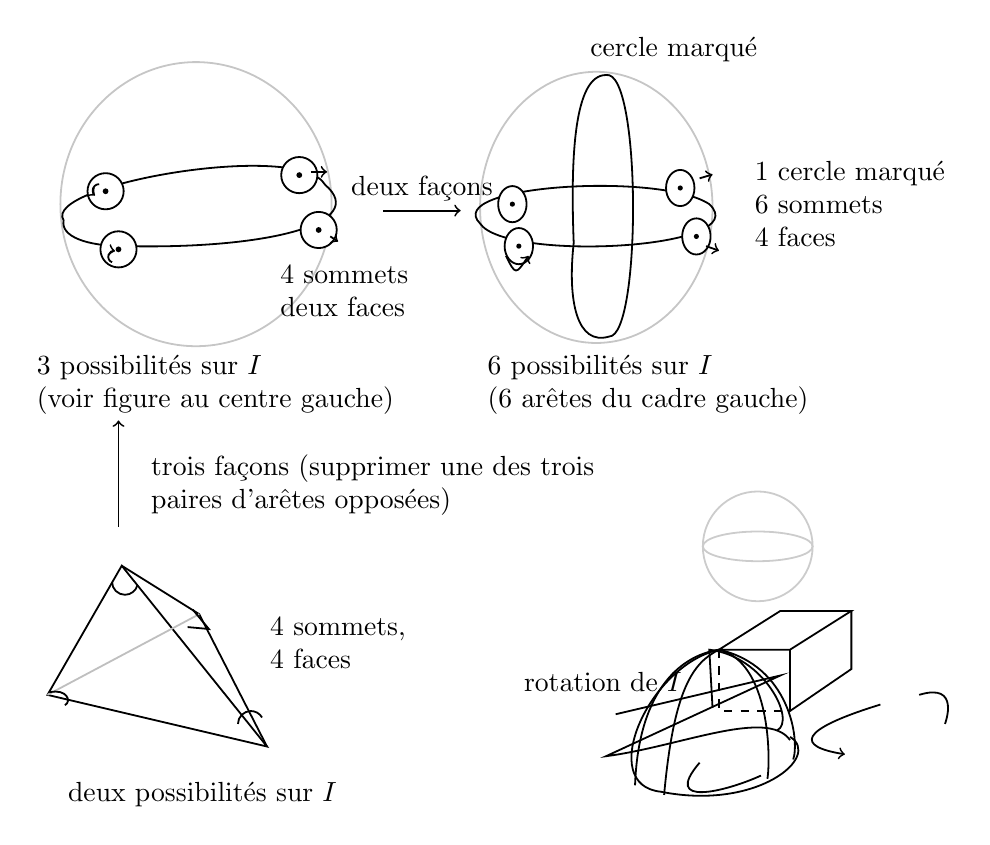
\begin{tikzpicture}[x=0.82cm,y=0.82cm,line width=.65pt]
\draw[gray!45] (2.3,8.7) ellipse (2.1 and 2.2);
\draw (0.25,8.45) .. controls (-.1,9) and (3.9,9.7) .. (4.3,9) .. controls (5,8.4) and (3.4,8) .. (1.2,8.05) .. controls (.6,8.05) and (.2,8.2) .. (.25,8.45);
\foreach \x/\y in {.9/8.9,1.1/8.0,3.9/9.15,4.2/8.3}{\draw[fill=white] (\x,\y) circle (.28);\fill (\x,\y) circle (.045);}
\draw[->] (.8,9.01) arc (90:230:.10);\draw[->] (1,7.8) arc (250:80:.09);\draw[->] (4.08,9.2)--(4.33,9.2);\draw[->] (4.38,8.2)--(4.5,8.12);
\node[align=left,anchor=west] at (3.45,7.35) {4 sommets\\deux faces};
\draw[->] (5.2,8.6)--(6.4,8.6) node[midway,above]{deux façons};
\draw[gray!45] (8.5,8.65) ellipse (1.8 and 2.1);
\draw (6.7,8.4) .. controls (6.1,9) and (9.5,9.2) .. (10.25,8.7) .. controls (11,8) and (7.1,7.8) .. (6.7,8.4);
\draw (8.15,8.1) .. controls (8.1,9.4) and (8.15,10.7) .. (8.65,10.7) .. controls (9.2,10.8) and (9.2,6.65) .. (8.7,6.65) .. controls (8.2,6.5) and (8.05,7.2) .. (8.15,8.1);
\foreach \x/\y in {7.2/8.7,7.3/8.05,9.8/8.95,10.05/8.2}{\draw[fill=white] (\x,\y) ellipse (.22 and .28);\fill (\x,\y) circle (.04);}
\draw[->] (7.1,7.9)..controls(7.25,7.6)..(7.45,7.9);\draw[->] (10.1,9.1)--(10.3,9.16);\draw[->](10.2,8.05)--(10.4,7.98);
\node at (9.7,11.1){\deleted{cercle marqué}};
\node[align=left,anchor=west] at (10.8,8.7){1 cercle marqué\\6 sommets\\4 faces};
\node[align=left] at (2.6,5.9){\uline{3 possibilités} sur $I$\\(\unsure{voir figure au centre gauche})};
\node[align=left] at (9.3,5.9){6 possibilités sur $I$\\(\unsure{6 arêtes du cadre gauche})};
\draw[->] (1.1,3.7)--(1.1,5.35);
\node[align=left,anchor=west] at (1.45,4.35){trois façons (supprimer une des trois\\\deleted{\unsure{paires}} d'arêtes opposées)};
\draw (0,1.1)--(1.15,3.1)--(3.4,.3)--cycle;
\draw (1.15,3.1)--(2.35,2.35)--(3.4,.3);\draw[gray!50](0,1.1)--(2.35,2.35);
\draw (1,2.85) arc(180:345:.2);\draw (2.17,2.15)--(2.5,2.12)--(2.25,2.42);\draw(.03,1.14)..controls(.3,1.2)and(.38,1)..(.27,.94);\draw(2.95,.65) arc(180:30:.2);
\node[align=left] at (4.5,1.9){4 sommets,\\4 faces};
\node at (2.4,-.45){deux possibilités sur $I$};
\draw[gray!40] (11,3.4) circle (.85);\draw[gray!40](11,3.4) ellipse(.85 and .23);
\draw (10.4,1.8)--(11.35,2.4)--(12.45,2.4)--(11.5,1.8)--cycle;\draw(11.5,1.8)--(11.5,.85)--(12.45,1.5)--(12.45,2.4);\draw[dashed](10.4,1.8)--(10.4,.85)--(11.5,.85);
\draw (10.4,1.8)..controls(9.3,1.55)and(8.5,-.3)..(9.5,-.4)..controls(11,-.7)and(12,.15)..(11.5,.45);
\draw(9.1,-.3)..controls(9.15,1.1)and(9.75,1.7)..(10.4,1.8)..controls(11.2,1.6)and(11.2,.1)..(11.15,-.2);
\draw(9.55,-.45)..controls(9.7,1.2)and(10,1.6)..(10.4,1.8)..controls(11.5,1.55)and(11.65,.4)..(11.55,.1);
\draw(10.3,.9)--(10.25,1.8)..controls(11.1,1.7)and(11.6,.7)..(11.3,.55);
\draw(8.8,.8)--(11.35,1.4)--(8.65,.15)..controls(9.8,.3)and(11.15,.9)..(11.5,.4);
\draw(10.1,.05)..controls(9.5,-.65)and(10.5,-.4)..(11.05,-.15);
\draw[->](12.9,.95)..controls(11.6,.55)and(11.6,.3)..(12.35,.18);\draw(13.5,1.1)..controls(14.15,1.3)and(13.9,.65)..(13.9,.65);
\node at (8.6,1.3){\deleted{\unsure{rotation de $I$}}};
\end{tikzpicture}}

\figure{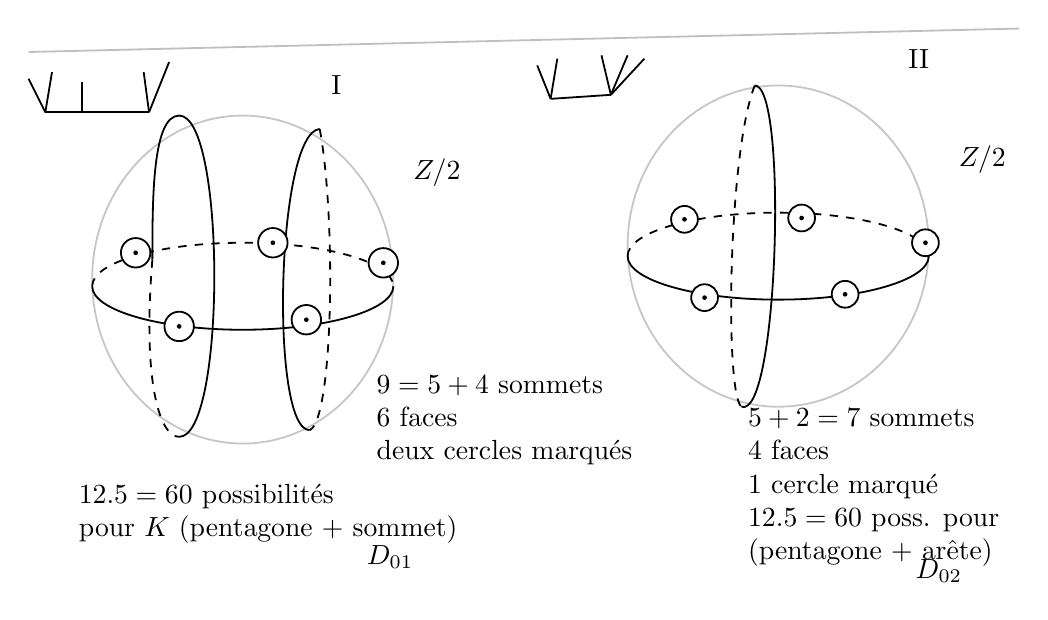
\begin{tikzpicture}[x=.85cm,y=.85cm,line width=.65pt]
\draw[gray!50](-.6,5.7)--(14.2,6.05);
\node at (4,5.2){I};\node at (12.7,5.6){II};
\draw(-.35,4.8)--(.6,4.8)--(1.2,4.8);\draw(-.35,4.8)--(-.6,5.3);\draw(-.35,4.8)--(-.25,5.4);\draw(.2,4.8)--(.2,5.25);\draw(1.2,4.8)--(1.12,5.4);\draw(1.2,4.8)--(1.5,5.55);
\draw(7.2,5)--(8.1,5.06);\draw(7.2,5)--(7,5.5);\draw(7.2,5)--(7.3,5.6);\draw(8.1,5.06)--(7.96,5.65);\draw(8.1,5.06)--(8.35,5.65);\draw(8.1,5.06)--(8.6,5.6);
\draw[gray!45] (2.6,2.3) ellipse(2.25 and 2.45);\draw (0.35,2.2) arc(180:360:2.25 and .65);\draw[dashed](.35,2.2) arc(180:0:2.25 and .65);
\draw(1.65,-.05)..controls(2.35,-.05)and(2.35,4.75)..(1.65,4.75)..controls(1.25,4.75)and(1.25,3.5)..(1.25,2.6);\draw[dashed](1.25,2.6)..controls(1.1,.8)and(1.35,-.05)..(1.65,-.05);
\draw(3.6,.05)..controls(3,.05)and(3.1,4.5)..(3.75,4.55);\draw[dashed](3.75,4.55)..controls(4,3.2)and(3.95,.2)..(3.6,.05);
\foreach \x/\y in {1/2.7,1.65/1.6,3.05/2.85,3.55/1.7,4.7/2.55}{\draw[fill=white](\x,\y) circle(.22);\fill(\x,\y)circle(.035);}
\node at (5.5,3.9){$\mathbb Z/2$};
\node[align=left,anchor=west] at (4.45,.2){$9=5+4$ sommets\\6 faces\\deux cercles marqués};
\node[align=left,anchor=west] at (0,-1.2){$12.5=\uline{60}$ possibilités\\pour $K$ (pentagone + sommet)};
\node at (4.8,-1.85){$D_{01}$};
\draw[gray!45](10.6,2.8) ellipse(2.25 and 2.4);\draw(8.35,2.65) arc(180:360:2.25 and .65);\draw[dashed](8.35,2.65) arc(180:0:2.25 and .65);
\draw(10.05,.4)..controls(10.6,.2)and(10.75,5.2)..(10.25,5.2);\draw[dashed](10.25,5.2)..controls(9.85,4.2)and(9.8,.6)..(10.05,.4);
\foreach \x/\y in {9.2/3.2,9.5/2.03,10.95/3.22,11.6/2.08,12.8/2.85}{\draw[fill=white](\x,\y)circle(.2);\fill(\x,\y)circle(.035);}
\node at (13.65,4.1){$\mathbb Z/2$};
\node[align=left,anchor=west] at (10,-.3){$5+2=7$ sommets\\4 faces\\1 cercle marqué};
\node[align=left,anchor=west] at (10,-1.55){$12.5=60$ poss. pour\\(pentagone + arête)};
\node at (13,-2.05){$D_{02}$};
\end{tikzpicture}}
\mspage{57}

\scanpage{59}
\begin{tabular}{c@{\qquad}l}
U N I V E R S I T E & MONTPELLIER, le 16 mars 1979\\
DES SCIENCES ET TECHNIQUES &\\
DU LANGUEDOC &\\
$\sim\sim\sim\sim\sim\sim\sim\sim\sim\sim\sim\sim$ &
\end{tabular}

Service de la Scolarité

MR/MG

\uline{Diffusion} : Liste H

N° 1634

\uline{AVIS DE SOUTENANCE D'UNE THESE DE DOCTORAT D'ETAT}

\uline{Nom et Prénom du candidat} : Monsieur LAIGNELET Bernard.

\uline{Titre de la thèse} : "Etude de certains facteurs biochimiques communs à la coloration et à la qualité culinaire des pâtes alimentaires de blé dur".

\uline{Date, heure et lieu de soutenance prévus} : Le 4 avril 1979 à 10 heures, Salle de Cours N° 9 U.S.T.L.

\uline{Nom du Directeur de la thèse} : Monsieur Pierre FEILLET.

\uline{Désignation du laboratoire où la thèse est préparée} : Laboratoire de Technologie des blés durs et du riz -INRA- Montpellier.

\uline{Résumé de la thèse} : Par des analyses statistiques et biochimiques, on montre qu'il n'existe pas de lien entre la coloration des pâtes alimentaires et les propriétés plastiques des pâtes et du gluten de blé dur.
Mais l'évolution de la coloration sous l'effet d'oxydations catalysées par les oxydoréductases présentes dans la semoule limiterait l'oxydation de la pâte et du gluten durant le pétrissage.

\uline{Durée approximative des recherches ayant abouti à la thèse} : 6 ans.

\uline{Noms des rapporteurs} :

M. CROUZET Jean\quad Directeur Scientifique, maître de conférences, Biochimie Alimentai-\\
\hspace*{3cm}re -U.S.T.L.-

M. ESCOUFIER Yves\quad Directeur Scientifique, maître de conférences, Statistique, -U.S.T.L.-

M. FEILLET Pierre\quad Directeur Ingénieur, maître de recherches, Technologie des Céréales -I.N.R A.-

\uline{Composition du jury} :

M. CROUZET J.\quad maître de conférences, Biochimie Alimentaire, U.S.T.L. (Président)

M. DRAPRON R.\quad Ingénieur 2° A, Biochimie Céréales, INRA\\
\hspace*{3cm}(Membre extérieur choisi en raison de sa compétence scientifique)

M. ECOCHARD R.\quad Professeur, Phytotechnie, E.N.S.A.T.

M. ESCOUFIER Y.\quad Maître de conférences, Statistiques, U.S.T.L.\\
\hspace*{3cm}(Membre étranger à la spécialité du candidat).

M. FEILLET P.\quad Maître de recherches, Technologie céréales,I.N.R.A.

Le Secrétaire Général,

MR LE PROFESSEUR GROTHENDIECK ALEX.

\unsure{E. Siau}

MATHEMATIQUES\qquad 5

\uline{E. SIAU}
\mspage{58}

\scanpage{60}
\figure{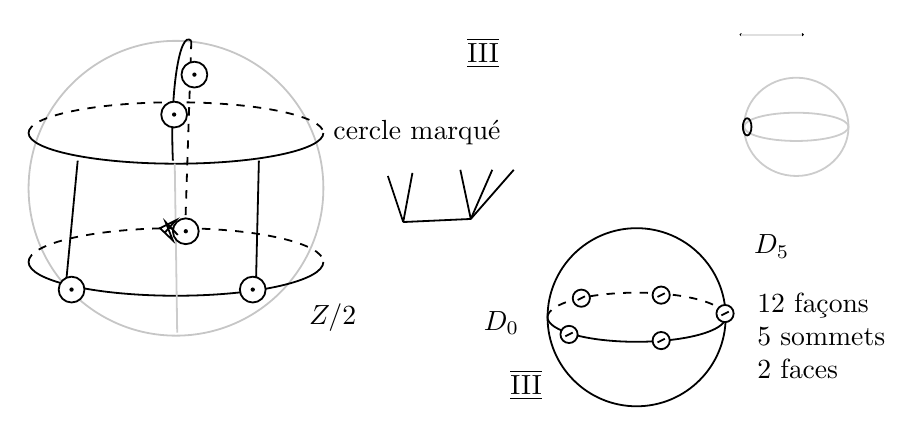
\begin{tikzpicture}[x=.78cm,y=.78cm,line width=.65pt]
\node at (8,6.2){$\underline{\overline{\mathrm{III}}}$};
\draw[gray!45](3,4)circle(2.4);\draw(0.6,4.9)arc(180:360:2.4 and .5);\draw[dashed](.6,4.9)arc(180:0:2.4 and .5);\draw(.6,2.8)arc(180:360:2.4 and .55);\draw[dashed](.6,2.8)arc(180:0:2.4 and .55);
\draw(1.4,4.45)--(1.2,2.35);\draw(4.35,4.45)--(4.3,2.35);\draw(2.95,4.45)..controls(2.9,5.5)and(3.05,6.6)..(3.25,6.4);\draw[dashed](3.25,6.4)--(3.15,3.35);\draw[gray!40](2.98,4.4)--(3.02,1.65);
\foreach \x/\y in {2.97/5.2,3.3/5.85,1.3/2.35,4.25/2.35,3.16/3.3}{\draw[fill=white](\x,\y)circle(.21);\fill(\x,\y)circle(.035);}
\draw(2.82,3.28)--(3,3.48)--(2.74,3.35)--(2.95,3.15)--(2.83,3.45)--(3.03,3.24);
\node[anchor=west]at(5.4,4.9){cercle marqué};\node at(5.55,1.9){$\mathbb Z/2$};
\draw(6.7,3.45)--(7.8,3.5);\draw(6.7,3.45)--(6.45,4.2);\draw(6.7,3.45)--(6.85,4.25);\draw(7.8,3.5)--(7.63,4.3);\draw(7.8,3.5)--(8.15,4.3);\draw(7.8,3.5)--(8.5,4.3);
\fill(12.2,6.5)circle(.025);\fill(13.2,6.5)circle(.025);\draw[gray!25](12.2,6.5)--(13.2,6.5);
\draw[gray!40](13.1,5)ellipse(.85 and .8);\draw[gray!40](13.1,5)ellipse(.85 and .23);\draw(12.3,5)ellipse(.07 and .14);
\draw(10.5,1.9)circle(1.45);\draw(9.05,1.9)arc(180:360:1.45 and .4);\draw[dashed](9.05,1.9)arc(180:0:1.45 and .4);
\foreach \x/\y in {9.6/2.21,9.4/1.62,10.9/2.26,10.9/1.52,11.94/1.96}{\draw[fill=white](\x,\y)circle(.14);\draw(\x-.06,\y-.03)--(\x+.06,\y+.03);}
\node at(8.3,1.8){$D_0$};\node at(12.7,3.05){$D_5$};\node at(8.7,.8){$\underline{\overline{\mathrm{III}}}$};
\node[align=left,anchor=west]at(12.3,1.6){\deleted{12 façons}\\5 sommets\\2 faces};
\end{tikzpicture}}

$9=3+3+1+2$ sommets\\6 faces\\1 cercle marqué

$60=10\times3\times2$ poss. pour $K$

\deleted{\unsure{K}} $(\underset{10}{\text{triangle}}+\underset{3}{\text{sommet marqué}}+\underset{2}{\text{1 sens de rot\unsure{.}}}$

\margin{\uline{12 possibilités} \unsure{qui définissent une} orientation de $K$}
\figure{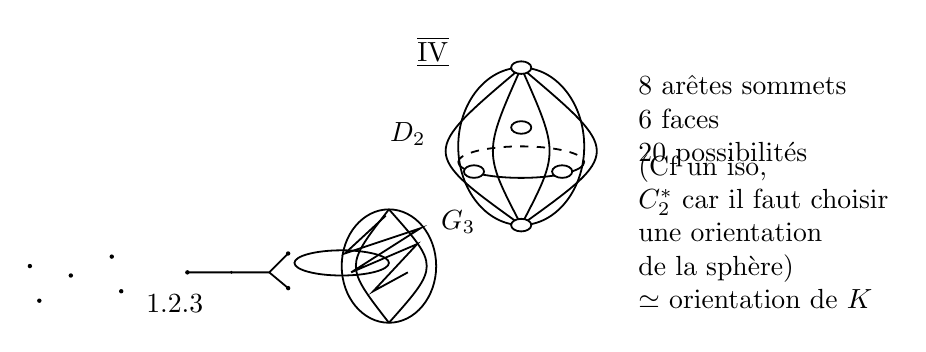
\begin{tikzpicture}[x=.8cm,y=.8cm,line width=.65pt]
\node at(6.4,3.1){$\underline{\overline{\mathrm{IV}}}$};\node at(6,1.8){$D_2$};
\draw(7.8,1.6)ellipse(1 and 1.25);\draw(7.8,2.85)..controls(6.2,1.5)..(7.8,.35);\draw(7.8,2.85)..controls(9.4,1.5)..(7.8,.35);\draw(7.8,2.85)..controls(7.2,1.5)..(7.8,.35);\draw(7.8,2.85)..controls(8.4,1.5)..(7.8,.35);\draw(6.8,1.35)arc(180:360:1 and .25);\draw[dashed](6.8,1.35)arc(180:0:1 and .25);
\foreach \x/\y in {7.8/2.85,7.8/1.9,7.05/1.2,8.45/1.2,7.8/.35}{\draw[fill=white](\x,\y)ellipse(.16 and .1);}
\node[align=left,anchor=west]at(9.5,2){$\unsure{8}$ \deleted{\unsure{arêtes}} sommets\\6 faces\\\uuline{20 possibilités}};
\node[align=left,anchor=west]at(9.5,.25){(\unsure{Cf un iso},\\\deleted{$\unsure{\mathbb C_2^*}$} car il faut choisir\\une orientation\\de la sphère)\\$\simeq$ orientation de $K$};
\draw(5.7,-.3)ellipse(.75 and .9);\draw(4.95,-.25)ellipse(.75 and .2);\draw(5.7,.6)..controls(5,-.3)..(5.7,-1.2);\draw(5.7,.6)..controls(6.5,-.3)..(5.7,-1.2);
\draw(5.65,.5)--(5,-.1)--(6.2,.3)--(5.1,-.4)--(6.15,.05)--(5.45,-.7)--(6,-.4);\node at(6.8,.4){$\unsure{G_3}$};
\foreach \x/\y in {0/-.3,.65/-.45,1.3/-.15,.15/-.85,1.45/-.7}{\fill(\x,\y)circle(.035);}
\draw(2.5,-.4)--(3.8,-.4)--(4.1,-.1);\draw(3.8,-.4)--(4.1,-.65);\fill(2.5,-.4)circle(.035);\fill(3.2,-.4)circle(.025);\fill(4.1,-.1)circle(.035);\fill(4.1,-.65)circle(.035);
\node at(2.3,-.9){\deleted{\unsure{$1.2.3$}}};
\end{tikzpicture}}

choisissons une orientation sur $K$, \deleted{\unsure{donc}} et bornons nous d'abord aux I, II avec pentagones compatibles avec l'orientation. Alors
\diagram{\begin{tikzcd}[ampersand replacement=\&]\deleted{\mathrm{II}}\arrow[r]\&\deleted{\mathrm I}\quad\deleted{\text{deux façons}}\end{tikzcd}}

donnée I $=$ sommet de l'icosaèdre \inserted{gauche $I_{C_\omega}$} $+$ arête \deleted{\unsure{qui en}} \inserted{incidente}, i.e. $\in D_{01}(I_{C_\omega})$
\margin{drapeaux de type 01}

donnée II $=$ sommet de l'icos. g. $+$ face \deleted{\unsure{qui en}} \inserted{incidente}, i.e. $\in D_{02}(I_{C_\omega})$

donnée III $=$ \deleted{\unsure{face}} \inserted{\unsure{tr. de}} \deleted{\unsure{arête}} de l'icos. g., \deleted{$+$ sommet dessus,}

\figure{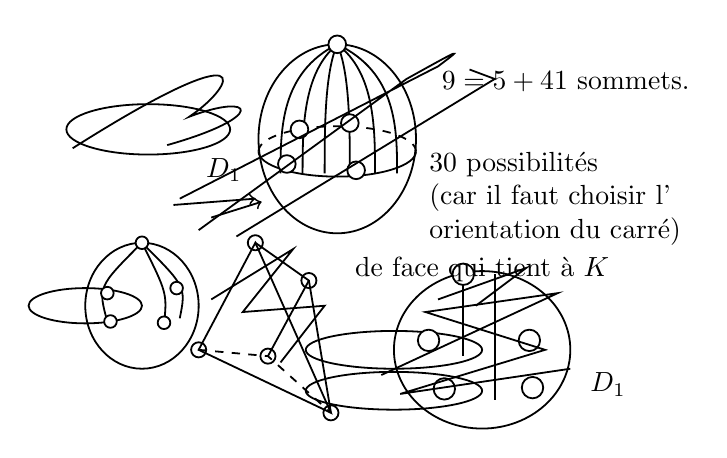
\begin{tikzpicture}[x=.8cm,y=.8cm,line width=.65pt]
\draw(5.7,3.4)ellipse(1.3 and .4);\draw(4.5,3.1)..controls(7.5,5)and(7.1,4.1)..(6.35,3.6)..controls(7.4,4)and(7.6,3.6)..(6,3.15);
\draw(8.7,3.25)ellipse(1.25 and 1.5);\draw(7.45,3.05)arc(180:360:1.25 and .4);\draw[dashed](7.45,3.05)arc(180:0:1.25 and .4);
\foreach \x in {7.8,8.15,8.5,8.9,9.3,9.65}{\draw(8.7,4.75)..controls(\x,4.3)and(\x,3.4)..(\x,2.7);}
\foreach \x/\y in {8.7/4.75,8.1/3.4,8.9/3.5,7.9/2.85,9/2.75}{\draw[fill=white](\x,\y)circle(.14);}
\draw(6.2,2.3)--(10.3,4.4)..controls(10.7,4.7)..(9.8,4.2)--(6.5,1.8);\draw(7.1,1.7)--(11.2,4.2)--(10.8,4.35);\draw[->](6.1,2.2)--(7.4,2.3);\draw[->](6.7,2)--(7.5,2.25);
\node at(6.9,2.75){$D_1$};\node[align=left,anchor=west]at(10.2,4.15){$9=5+4$\deleted{\unsure{1}} sommets.};
\node[align=left,anchor=west]at(10,2.3){30 possibilités\\(car il faut choisir l'\\orientation du carré)};
\draw(5.6,.6)ellipse(.9 and 1);\draw(4.7,.6)ellipse(.9 and .28);\draw(5.6,1.6)..controls(4.9,.9)..(5.05,.35);\draw(5.6,1.6)..controls(6.3,.9)..(6.2,.4);\draw(5.6,1.6)..controls(6,.8)..(5.95,.3);
\foreach \x/\y in {5.6/1.6,5.05/.8,6.15/.88,5.1/.35,5.95/.33}{\draw[fill=white](\x,\y)circle(.1);}
\draw(6.5,-.1)--(7.4,1.6)--(8.6,-1.1)--cycle;\draw(7.4,1.6)--(8.25,1)--(8.6,-1.1);\draw[dashed](6.5,-.1)--(7.6,-.2)--(8.6,-1.1);\draw(8.25,1)--(7.6,-.2);\foreach\x/\y in{6.5/-.1,7.4/1.6,8.25/1,8.6/-1.1,7.6/-.2}{\draw(\x,\y)circle(.12);}\draw(6.7,.7)--(8,1.5)--(7.2,.5)--(8.5,.6)--(7.8,-.3);
\draw(11,-.1)ellipse(1.4 and 1.25);\draw(9.6,-.1)ellipse(1.4 and .3);\draw(9.6,-.75)ellipse(1.4 and .3);\draw(10.7,1.15)--(10.7,-.2);\draw(11.2,1.1)--(11.2,-.9);\foreach\x/\y in{10.7/1.1,10.15/.05,11.75/.05,10.4/-.72,11.8/-.7}{\draw[fill=white](\x,\y)circle(.17);}\draw(9.4,-.5)--(12.2,.8)--(10.1,.5)--(12,-.1)--(9.7,-.8)--(12.4,-.4);\draw(10.3,.7)--(11.7,1.2)--(10.9,.6);\node at(13,-.65){$D_1$};
\node at(11,1.18){\deleted{\unsure{de face qui tient à $K$}}};
\end{tikzpicture}}
\diagram{\begin{tikzcd}[ampersand replacement=\&, row sep=small]
\deleted{D_0}\arrow[r]\&\deleted{D_1}\quad\deleted{\text{cinq façons}}\\
\deleted{D_1}\arrow[r]\&\deleted{D_2}\\
D_{01}\arrow[r]\&D_0\\
D_{01}\arrow[r,no head]\&D_1\\
D_{02}\arrow[r,no head]\&D_0\\
D_{02}\arrow[r,no head]\&D_2\quad\deleted{\uuline{\unsure{bipartité}}}
\end{tikzcd}}
\mspage{59}

\scanpage{61}
\begin{tabular}{c@{\qquad}l}
U N I V E R S I T E & MONTPELLIER, le 31 MAI 1979\\
DES SCIENCES ET TECHNIQUES &\\
DU LANGUEDOC &\\
\texttt{------------} &
\end{tabular}

Service de la Scolarité\\
MR / GJ\\
Diffusion : Liste A\\
N° : 3159

\uline{AVIS DE SOUTENANCE D'UNE THESE DE DOCTEUR INGENIEUR}

\uline{Chimie industrielle - l'Eau et les Nuisances}

\uline{Nom et prénom du candidat} : B L A N C H E T O N\quad J e a n - P a u l

\uline{Titre de la thèse} : Analyse du fonctionnement d'un étang-solaire par modélisation à partir de données recueillies sur un étang expérimental à Palavas.

\uline{Date, heure et lieu de soutenance prévus} : 12 JUIN 1979 à 14 Heures 30 mn\\
Salle de cours n° 9 - U.S.T.L.

\uline{Nom du Directeur de thèse} : Monsieur le Professeur BOCQUILLON Claude.

\uline{Désignation du laboratoire où la thèse est préparée:}\\
Laboratoire d'Hydrologie Mathématique

\uline{Résumé de la thèse} :

L'étang-solaire est un capteur solaire constitué d'un bassin peu profond, partiellement transparent au rayonnement solaire, et dont les pertes thermiques sont réduites en éliminant les phénomènes convectifs par un gra-\\
dient salin et stabilisateur.

Plusieurs de ces bassins ont déjà été étudiés dans le monde. Un bassin expérimental a été construit à Palavas et exploité en collaboration, par l'Université des Sciences et Techniques du Languedoc, le Centre National pour l'Exploitation des Océans et la Société ELF.

Deux campagnes de mesures, de mars 1977 à décembre 1977 et de mars 1978 à mai 1979, ont permis de résoudre les problèmes technologiques de mise en place et maintien de la stratification saline, et de suivre l'évolution thermique du milieu.

Cette expérimentation a rendu possible la mise au point d'un modèle d'évolution d'un tel bassin à partir de la connaissance des données géographiques, météorologiques et techniques du bassin.

Des tests de validité ont montré l'exactitude du modèle. Des simulations ont permis la définition des rendements du système sous diverses conditions du fonctionnement (\textit{température d'extraction,quantité de chaleur extraite}).

\uline{Durée approximative des recherches ayant abouti à la thèse} : 2 ans et demi.

\uline{Composition du jury proposé} :
\begin{tabular}{lll}
MM.:& BEN AIM & R.\\
& BOCQUILLON & Cl.\\
& HYACINTHE & J-L.\\
& DE CHABERT & F.\\
& ROUSSEL & A.\\
& PERRUT & M.\\
& RONC & M.
\end{tabular}

Le Secrétaire Général,

\unsure{E S}

\uline{E. S I A U}
\mspage{60}

\scanpage{62}
\figure{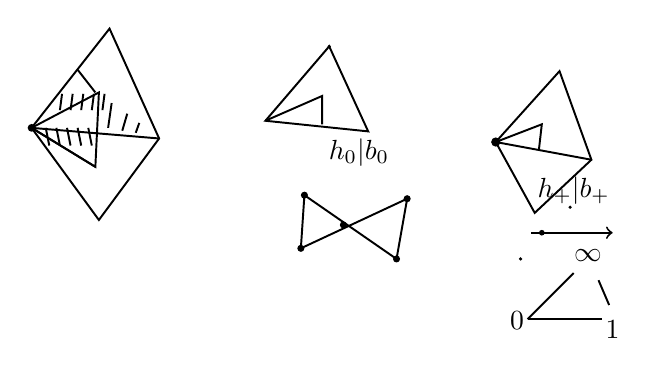
\begin{tikzpicture}[x=.9cm,y=.9cm,line width=.7pt]
\draw(0,1.6)--(1.1,3)--(1.8,1.45)--(.95,.3)--cycle;\draw(0,1.6)--(1.8,1.45);\draw(0,1.6)--(.95,2.1)--(.9,1.05)--cycle;\draw(.65,2.42)--(.9,2.1);\draw(0,1.6)--(.9,1.05);\foreach \x in {.2,.35,.5,.65,.8}{\draw(\x,1.6)--(\x+.05,1.35);\draw(\x+.2,1.85)--(\x+.23,2.08);} \draw(1.08,1.6)--(1.13,1.95);\draw(1.28,1.56)--(1.35,1.8);\draw(1.47,1.53)--(1.52,1.67);\fill(0,1.6)circle(.055);
\draw(3.3,1.7)--(4.2,2.75)--(4.75,1.55)--cycle;\draw(3.3,1.7)--(4.1,2.05)--(4.1,1.65);\fill(4.2,2.75)circle(.025);\node at(4.62,1.25){$\unsure{h_0|b_0}$};
\draw(3.85,.65)--(3.8,-.1)--(5.3,.6)--(5.15,-.25)--cycle;\foreach\x/\y in{3.85/.65,3.8/-.1,4.4/.23,5.3/.6,5.15/-.25}{\fill(\x,\y)circle(.05);}
\draw(6.55,1.4)--(7.45,2.4)--(7.9,1.15)--(7.1,.4)--cycle;\draw(6.55,1.4)--(7.9,1.15);\draw(6.55,1.4)--(7.2,1.65)--(7.16,1.3);\fill(6.55,1.4)circle(.065);\node at(7.65,.72){$\unsure{h_+|b_+}$};\draw[->](7.05,.12)--(8.2,.12);\fill(7.2,.12)circle(.04);\fill(6.9,-.25)circle(.025);\fill(7.6,.48)circle(.025);
\draw(7,-1.1)--(8.05,-1.1);\draw(7,-1.1)--(7.65,-.45);\draw(8,-.55)--(8.15,-.9);\node at(6.85,-1.12){$0$};\node at(7.85,-.2){$\infty$};\node at(8.2,-1.25){$1$};
\end{tikzpicture}}

\diagram{\begin{tikzcd}[ampersand replacement=\&]\mathbb Z/5\mathbb Z\arrow[d]\\D_5\end{tikzcd}}
($D_5\times\mathbb Z/2\mathbb Z$ dans \unsure{théo. non orientée}
\figure{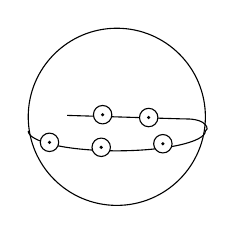
\begin{tikzpicture}[scale=.9]
\draw(0,0)circle(1.25);\draw(-1.25,-.2)arc(180:360:1.25 and .28);\draw(-.7,.02)--(.95,-.03)..controls(1.3,-.02)and(1.3,-.2)..(1.25,-.2);
\foreach\x/\y in{-.95/-.36,-.22/-.43,.65/-.38,-.2/.03,.45/-.01}{\draw[fill=white](\x,\y)circle(.13);\fill(\x,\y)circle(.025);}
\end{tikzpicture}}
12 possibilités \deleted{\unsure{K}} (struct. pentag. sur $K$)

(\uline{NB} \deleted{\unsure{les}} 12 sommets de l'icos. le stabilisateur d'un sommet est $\mathbb Z/5\mathbb Z$, \deleted{\unsure{d'ordre $\mathbb Z/5\mathbb Z$}} \inserted{et dans le cas non orienté} $D_5$)
\margin{\uline{Implique \unsure{orientation} de $K$}}

$\mathbb Z/4\mathbb Z$

($D_4$ dans théorie non orientée)
\figure{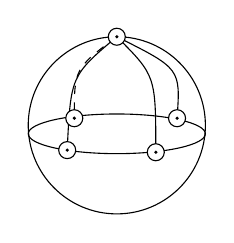
\begin{tikzpicture}[scale=.9]
\draw(0,0)circle(1.25);\draw(0,-.12)ellipse(1.25 and .28);\draw(0,1.25)..controls(-.65,.7)..(-.7,-.35);\draw(0,1.25)..controls(.9,.8)..(.85,.1);\draw(0,1.25)..controls(.55,.7)..(.55,-.38);\draw[dashed](0,1.25)..controls(-.6,.8)..(-.6,.1);
\foreach\x/\y in{0/1.25,-.6/.1,.85/.1,-.7/-.35,.55/-.38}{\draw[fill=white](\x,\y)circle(.12);\fill(\x,\y)circle(.025);}
\end{tikzpicture}}
$30=15\times2$ possibilités (\inserted{\uline{structure en}} carrés orientés dans $K$)

(\uline{NB} 30 arêtes de l'icosaèdre, le stabilisateur d'un sommet est $\mathbb Z/2\mathbb Z$ (et $D_2=\mathbb Z/2\times\mathbb Z/2$ au cas non orienté)

\uline{n'implique pas d'orientation de $K$}

\diagram{\begin{tikzcd}[ampersand replacement=\&]\mathbb Z/3\mathbb Z\arrow[d]\\\unsure{\mathfrak S_3|G_3}\end{tikzcd}}
($D_3\times\mathbb Z/2\mathbb Z$ en théorie non orientée
\figure{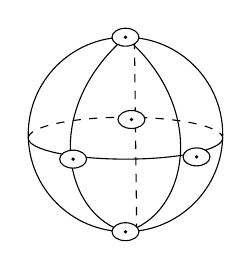
\begin{tikzpicture}[scale=.95]
\draw(0,0)circle(1.3);\draw(-1.3,-.05)arc(180:360:1.3 and .28);\draw[dashed](-1.3,-.05)arc(180:0:1.3 and .28);\draw(0,1.3)..controls(-1.15,.3)and(-.8,-1.1)..(0,-1.3);\draw(0,1.3)..controls(1.15,.3)and(.8,-1.1)..(0,-1.3);\draw[dashed](.12,1.25)--(.15,-1.25);
\foreach\x/\y in{0/1.3,.08/.2,-.7/-.33,.95/-.3,0/-1.3}{\draw[fill=white](\x,\y)ellipse(.18 and .12);\fill(\x,\y)circle(.025);}
\end{tikzpicture}}
$20=10\times$ possibilités (triangles de $K$ \deleted{\unsure{pas de nature}} \inserted{orientés} de $K$) (NB 20 faces de l'icosaèdre, stabilisateur de chacune est $\mathbb Z/3\mathbb Z$ ; groupe $\unsure{\mathfrak S_3|G_3}$ cas non orienté)
\mspage{61}

\scanpage{63}
\figure{\begin{tikzpicture}\draw(0,0)--(1.1,0);\end{tikzpicture}}

Avant de me lancer vers une exploitation des principes dégagés, il me faut encore développer le formalisme des ``points base à l'infini''. Le point de départ est le suivant. \deleted{\unsure{Et}} (NB je me borne pour l'instant à la dim 1, \deleted{bien que} \inserted{mais} il sera nécessaire de revenir par la suite sur les phénomènes analogues en dimension quelconque, relatifs à la donnée d'un diviseur à croisements normaux\ldots) Soit $X$ un schéma local régulier de dim 1 (i.e. le spectre d'un anneau \unsure{rég.} \inserted{$A$}), et $x$ son point fermé, $k=k(x)$,
\inserted{on suppose $k$ de car. nulle}
\deleted{$\unsure{U=}$}
\[
\tag{53} U=X\setminus\{x\}=\{\eta\}
\]
l'ouvert réduit au point générique, et
\[
\tag{54} T_x=\mathbf V(\mathfrak m_x/\mathfrak m_x^2)
=\check{\mathbf V}\bigl(\unsure{(\mathfrak m_x/\mathfrak m_x^2)|(\mathfrak m_x/\mathfrak m_x^2)^\vee}\bigr)
\]
le $k$-schéma ``espace tangent en $x$'', \inserted{$T_x^*=T_x\setminus\{0\}$,} je dis qu'on a alors un morphisme canonique
\[
\tag{55} \widehat\Pi_1(T_x^*)\longrightarrow\widehat\Pi_1(U)
\]
(où les $\widehat\Pi_1$ ici sont les $\Pi_1$ schématiques).

On est \unsure{ramené} \unsure{d'emblée} au cas où $A$ est \deleted{\unsure{\textup{à. A} est}} complet \deleted{\unsure{et alors}} (puisque $\widehat U\longrightarrow U$ donc $\widehat\Pi_1(\widehat U)\mathrel{-}\widehat\Pi_1(U)$)

Alors on sait qu'on a \unsure{!|:}
\mspage{62}

\scanpage{64}
\figure{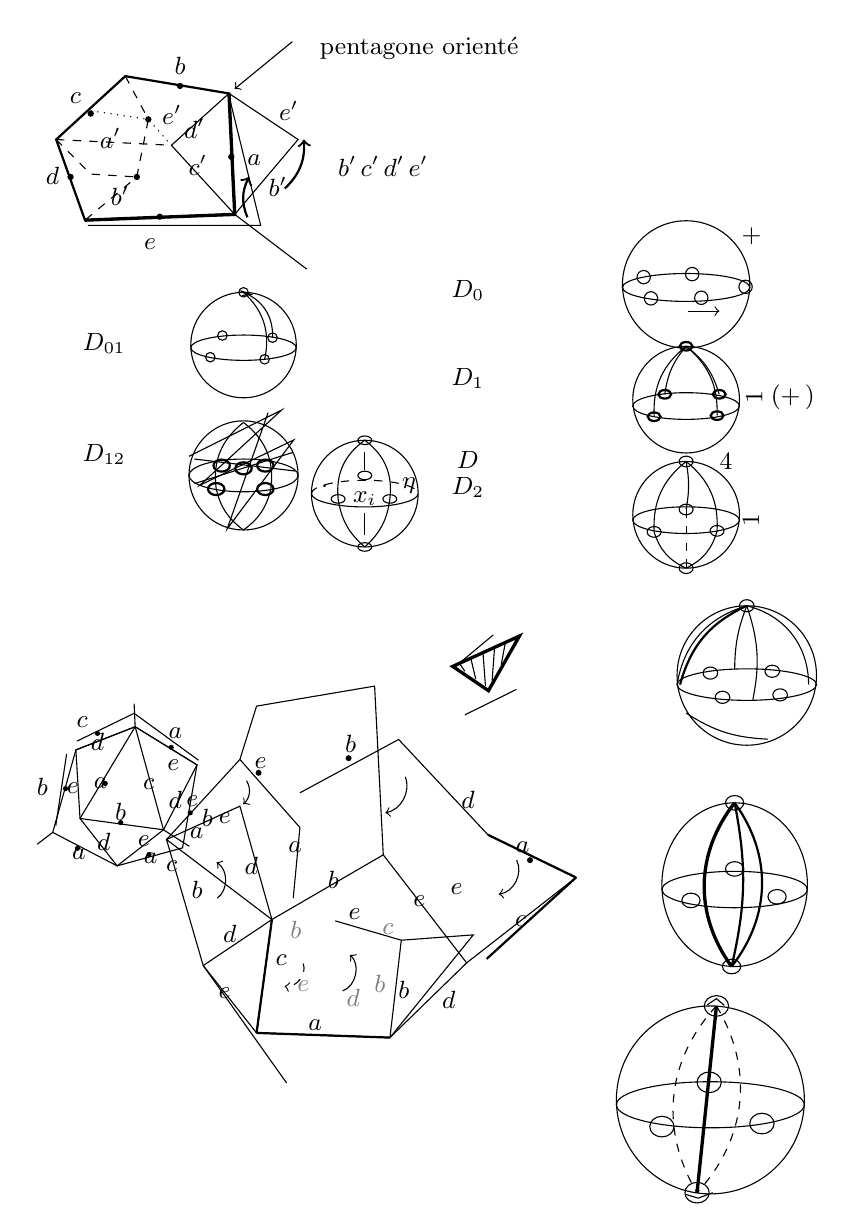
\begin{tikzpicture}[scale=.77, every node/.style={font=\small}]
\node[anchor=west] at(5.1,1.7){pentagone orienté};
\node at(6.3,-.25){$b'\,c'\,d'\,e'$};
\begin{scope}[shift={(3,0)},scale=.95]
\draw[thick](-1,1.3)--(.8,1)--(.9,-1.1)--(-1.7,-1.2)--(-2.2,.2)--cycle;
\draw[very thick](.8,1)--(.9,-1.1)--(-1.7,-1.2);
\draw(.8,1)--(2,.2)--(.9,-1.1);
\draw(.8,1)--(-.2,.1)--(.9,-1.1);
\draw[dashed](-1,1.3)--(-.6,.55)--(-.8,-.45)--(-1.7,-1.2);
\draw[dashed](-2.2,.2)--(-.2,.1);
\draw[dashed](-2.2,.2)--(-1.6,-.4)--(-.8,-.45);
\draw[dotted](-1.6,.7)--(-.6,.55)--(-.2,.1);
\draw[->](1.9,1.9)--(.9,1.08);
\draw(.9,-1.1)--(2.15,-2.05);
\draw[->,thick](1.12,-1.15) to[bend left=25](1.15,-.45);
\draw[->,thick](1.77,-.65) to[bend right=25](2.1,.2);
\draw(-1.65,-1.29)--(1.35,-1.29)--(.8,.96);
\foreach \p in {(.84,-.1),(-.05,1.13),(-1.6,.65),(-1.95,-.45),(-.4,-1.14),(-.6,.55),(-.8,-.45)} \fill\p circle(.055);
\node[right]at(.95,-.16){$a$}; \node[above]at(-.05,1.16){$b$};\node[above left]at(-1.6,.65){$c$};\node[left]at(-1.98,-.43){$d$};\node[below]at(-.57,-1.35){$e$};
\node at(-1.26,.22){$a'$};\node[below left]at(-.76,-.44){$b'$};\node at(.26,-.25){$c'$};\node at(.2,.39){$d'$};\node[right]at(-.53,.63){$e'$};\node[right]at(1.5,.7){$e'$};\node at(1.65,-.62){$b'$};
\end{scope}
\node at(1.7,-3.18){$D_{01}$};
\begin{scope}[shift={(4,-3.2)},scale=.87]
\draw(0,0)circle(1);\draw(0,-.05)ellipse(1 and .24);
\draw(0,1)to[bend left=30](.4,-.27);\draw(0,1)to[bend left=35](.55,.14);
\foreach\p in{(0,1),(-.4,.18),(.55,.14),(-.63,-.23),(.4,-.27)}\draw\p circle(.09);
\draw(-.06,1.03)--(.14,.96)--(-.03,.94);
\end{scope}
\node at(1.7,-5){$D_{12}$};
\begin{scope}[shift={(4,-5.35)},scale=.9]
\draw(0,0)circle(1);\draw(0,0)ellipse(1 and .3);\draw(0,.97)to[bend right=30](-.5,-.25)to[bend right=20](0,-1);\draw(0,.97)to[bend left=30](.5,-.25)to[bend left=20](0,-1);
\foreach\p in{(-.4,.18),(.4,.18),(-.5,-.25),(.4,-.25),(0,.13)}\draw[thick]\p ellipse(.15 and .11);
\draw(-1,.35)--(.7,1.2)--(-.8,-.18)--(.92,.65)--(-.3,-.98)--(.45,1.15);
\draw(-.9,.3)--(.95,.08);\draw(-.9,-.15)--(.9,.42);
\end{scope}
\begin{scope}[shift={(6,-5.65)},scale=.88]
\draw(0,0)circle(1);\draw[dashed](-1,0)arc(180:0:1 and .25);\draw(-1,0)arc(180:360:1 and .25);
\draw(0,1)to[bend right=30](-.5,-.1)to[bend right=20](0,-1);\draw(0,1)to[bend left=30](.47,-.1)to[bend left=20](0,-1);
\draw(0,.78)--(0,.45);\draw(0,-.37)--(0,-.78);
\foreach\p in{(0,1),(0,-1),(-.5,-.1),(.47,-.1),(0,.34)}\draw\p ellipse(.13 and .08);
\node at(0,-.1){$x_i$};\node at(.83,.16){$\unsure{\eta}$};\node at(-.75,.13){$\unsure{\cdot}$};
\end{scope}
\node at(7.7,-5.1){\deleted{$\unsure{D}$}};
\node at(7.7,-5.55){$D_2$};
\node at(7.7,-2.3){$D_0$};\node at(7.7,-3.75){$D_1$};
\begin{scope}[shift={(11.3,-2.2)}]
\draw(0,0)circle(1.05);\draw(0,-.05)ellipse(1.05 and .23);
\foreach\p in{(-.7,.12),(.1,.17),(.98,-.04),(-.58,-.23),(.25,-.22)}\draw\p circle(.11);
\draw[->](.03,-.44)--(.55,-.44);\node at(1.08,.8){$+$};
\end{scope}
\begin{scope}[shift={(11.3,-4.1)},scale=.88]
\draw(0,0)circle(1);\draw(0,-.12)ellipse(1 and .25);
\draw(0,1)to[bend right=27](-.6,-.32);\draw(0,1)to[bend right=16](-.4,.1);\draw(0,1)to[bend left=26](.58,-.3);\draw(0,1)to[bend left=18](.62,.1);
\foreach\p in{(0,1),(-.6,-.32),(-.4,.1),(.58,-.3),(.62,.1)}\draw[thick]\p ellipse(.12 and .08);
\node[rotate=90]at(1.28,.05){\deleted{\unsure{\illegible{1}}}};\node at(2,.05){$(+\,\circlearrowleft)$};
\end{scope}
\begin{scope}[shift={(11.3,-6)},scale=.88]
\draw(0,0)circle(1);\draw(0,-.1)ellipse(1 and .25);
\draw(0,1)to[bend right=27](-.6,-.32)to[bend right=24](0,-1);\draw(0,1)to[bend left=27](.58,-.3)to[bend left=24](0,-1);
\draw(0,1)to[bend left=10](0,.1);\draw[dashed](0,.1)--(0,-1);
\foreach\p in{(0,1),(0,-1),(-.6,-.32),(.58,-.3),(0,.1)}\draw\p ellipse(.13 and .1);
\node at(.75,1){$\unsure{4}$};\node[rotate=90]at(1.22,-.1){\deleted{\unsure{\illegible{1}}}};
\end{scope}
\begin{scope}[shift={(8,-8.5)}]
\draw[very thick](-.55,0)--(.55,.5)--(.04,-.4)--cycle;
\draw(-.44,.05)--(-.35,-.08);\draw(-.25,.13)--(-.17,-.21);\draw(-.05,.22)--(-.01,-.32);\draw(.14,.31)--(.1,-.24);\draw(.32,.4)--(.25,.03);
\draw[thin](-.35,-.8)--(.5,-.38);\draw(-.48,.02)--(.12,.52);
\end{scope}
\begin{scope}[shift={(12.3,-8.65)}]
\draw[thin](0,0)circle(1.15);\draw[thin](0,-.15)ellipse(1.15 and .26);
\draw[thick](0,1.15)to[bend right=25](-1.1,-.15);\draw[thin](0,1.15)to[bend right=32](-1.15,-.15);\draw(0,1.15)to[bend left=15](.1,-.4);\draw[thin](0,1.15)to[bend right=10](-.2,.1);\draw[thin](0,1.15)to[bend left=38](1.02,-.15);
\foreach\p in{(0,1.15),(-.6,.04),(.42,.07),(-.4,-.36),(.55,-.32)}\draw\p ellipse(.12 and .1);
\draw[thin](-1,-.62)to[bend right=15](.35,-1.05);
\end{scope}
\begin{scope}[shift={(2,-10.6)},scale=.85]
\draw(-.9,.85)--(.25,1.3)--(1.45,.56)--(1.17,-1.05)--(-.1,-1.4)--(-1.35,-.75)--cycle;
\draw(-.9,.85)--(-.82,-.48)--(.8,-.7)--(.25,1.3)--cycle;
\draw(-.82,-.48)--(.25,1.3)--(1.45,.56)--(.8,-.7)--(-.1,-1.4)--(-.82,-.48);
\draw(-1.35,-.75)--(-1.65,-.98);\draw(.25,1.3)--(.23,1.75);\draw(.8,-.7)--(1.3,-1.02);
\draw(-.88,1.02)--(.23,1.56)--(1.48,.65);\draw(-1.29,-.62)--(-1.08,.77);
\foreach\p in{(-.48,1.17),(.95,.9),(-1.1,.1),(-.33,.2),(-.03,-.56),(-.87,-1.06),(.52,-1.18),(1.32,-.37)}\fill\p circle(.05);
\node at(-.78,1.39){$c$};\node at(-.48,1){$d$};\node at(1.03,1.17){$a$};\node at(.99,.55){$e$};\node at(-1.55,.13){$b$};\node at(-.96,.11){$\unsure{e}$};\node at(-.42,.21){$a$};\node at(.51,.18){$c$};\node at(1.03,-.12){$d$};\node at(1.36,-.15){$\unsure{e}$};\node at(1.65,-.47){$b$};\node at(1.99,-.48){\deleted{$\unsure{e}$}};
\node at(-.03,-.35){$b$};\node at(-.84,-1.18){$a$};\node at(-.36,-.94){$d$};\node at(.42,-.92){$e$};\node at(.55,-1.25){$a$};\node at(.96,-1.4){$c$};
\end{scope}
\begin{scope}[shift={(5.7,-13.5)},scale=1.1]
\draw[thin](-1.35,-.95)--(.65,-1.02)--(1.8,.1)--(.55,1.72)--(-1.12,.75)--cycle;
\draw[thick](-1.35,-.95)--(.65,-1.02);\draw[thick](-1.35,-.95)--(-1.12,.75);
\draw[thin](-1.12,.75)--(-2.7,1.95)--(-1.6,3.15)--(-.7,2.13)--(-.8,1.07);
\draw[thin](-1.6,3.15)--(-1.35,3.95)--(.42,4.25)--(.55,1.72);
\draw[thin](-.7,2.65)--(.78,3.45)--(2.12,2.02)--(3.44,1.38)--(1.8,.1);
\draw[thin](-2.7,1.95)--(-2.15,.06)--(-1.35,-.95);\draw[thin](-2.7,1.95)--(-1.6,2.45)--(-1.12,.75)--(-2.15,.06);
\draw[thick](2.12,2.02)--(3.44,1.38);\draw[thick](3.44,1.38)--(2.1,.16);
\draw[thin](-1.12,.75)--(-1.35,-.95)--(.65,-1.02)--(.82,.44)--(-.17,.73);
\draw[thin](-2.15,.06)--(-.9,-1.7);\draw[thin](.65,-1.02)--(1.9,.52)--(.82,.44);
\draw[->](-.06,-.32)to[bend right=60](.05,.22);\draw[->,dashed](-.65,.09)to[bend left=60](-.93,-.25);
\draw[->](-1.94,1.07)to[bend right=55](-1.95,1.61);\draw[->](2.55,1.64)to[bend left=55](2.28,1.13);\draw[->](.88,2.89)to[bend left=50](.58,2.35);\draw[->](-1.5,2.83)to[bend left=40](-1.55,2.48);
\foreach\p in{(-1.32,2.95),(.03,3.17),(2.75,1.64)}\fill\p circle(.045);
\node at(-.47,-.84){$a$};\node at(-.98,.14){$c$};\node at(.86,-.3){$b$};\node at(1.53,-.45){$d$};\node at(-1.83,-.35){$e$};\node at(-1.75,.54){$d$};\node at(-2.24,1.2){$b$};\node at(-2.25,2.04){$a$};\node at(-1.43,1.56){$d$};\node at(-.77,1.83){$a$};\node at(-1.29,3.1){$e$};\node at(.06,3.38){$b$};\node at(1.82,2.54){$d$};\node at(2.64,1.83){$a$};\node at(2.61,.73){$c$};\node at(1.65,1.21){$e$};\node at(1.09,1.03){$e$};\node at(-.2,1.34){$b$};\node at(.12,.83){$\unsure{e}$};
\node[text=gray]at(-.76,.6){$\unsure{b}$};\node[text=gray]at(.62,.6){$\unsure{c}$};\node[text=gray]at(.5,-.21){$b$};\node[text=gray]at(.1,-.43){$d$};\node[text=gray]at(-.65,-.25){$\unsure{e}$};
\end{scope}
\begin{scope}[shift={(12.1,-12.1)}]
\draw[thin](0,0)ellipse(1.2 and 1.35);\draw[thin](0,-.08)ellipse(1.2 and .3);
\draw[very thick](0,1.35)to[bend right=37](-.05,-1.35);\draw[thick](0,1.35)to[bend left=37](-.05,-1.35);\draw[thick](0,1.35)to[bend left=12](-.05,-1.35);
\foreach\p in{(0,1.35),(-.05,-1.35),(-.72,-.26),(.7,-.2),(0,.26)}\draw\p ellipse(.15 and .12);
\end{scope}
\begin{scope}[shift={(11.7,-15.65)}]
\draw[thin](0,0)circle(1.55);\draw[thin](0,-.08)ellipse(1.55 and .38);
\draw[very thick](.1,1.55)--(-.22,-1.53);\draw[dashed](.1,1.55)to[bend right=37](-.22,-1.53);\draw[dashed](.1,1.55)to[bend left=37](-.22,-1.53);
\foreach\p in{(.1,1.55),(-.22,-1.53),(-.8,-.44),(.85,-.39),(-.02,.29)}\draw\p ellipse(.2 and .17);
\draw(-.05,1.57)--(.1,1.67)--(.23,1.56);\draw(-.4,-1.56)--(-.2,-1.62)--(.04,-1.53);
\end{scope}
\end{tikzpicture}}
\mspage{63}

\scanpage{65}
\unsure{mes b.r.} étaient $0,\infty$ au lieu de $0,1$, et la troisième \unsure{borne} (im. \unsure{pt} de $0,\infty$ sur $\mathbb X_1$) était $1$ au lieu de $\infty$,
\deleted{\unsure{ici on avait --- $\mathbb X_1$ au but et non $\mathbb X_0$}}, l'application cherchée serait donnée par (25) $z\longmapsto z^2$;
\inserted{modulo composition avec des transformations homographiques}
\deleted{\unsure{il aurait à donner} \unsure{composée avec l'isomorphisme}}
\[
g_1(z)=\psi\bigl(\varphi(z)^2\bigr),\quad\unsure{-}
\]
\deleted{(application homographique) qui réalise}
où $\psi$ est l'application homographique qui réalise
\[
0\quad1\quad\infty\quad\longrightarrow\quad0\quad\infty\quad1
\]
\deleted{i.e.}
\[
\deleted{\psi(z)=\sigma_0(z)=\frac{\unsure{z}}{\unsure{z-1}},}
\]
et où $\varphi$ est l'application homographique qui réalise
\deleted{donc on trouve}
\[
1\longrightarrow0,\quad-1\longmapsto\infty,\quad0\,(\text{ou }\infty)\longrightarrow1
\]
\[
\deleted{\mathbb X_1\longrightarrow\mathbb X_0\quad z\longmapsto\frac{z^2}{\unsure{z^2-1}}}
\]
donc
\[
\psi(z)=\sigma_0(z)=\frac{z}{z-1},\qquad\varphi(z)=\frac{z-1}{z+1}
\]
et en composant l'application cherchée
\[
\tag{26}
\left\{\begin{aligned}
g_1&:\mathbb X_1\longrightarrow\mathbb X_0:\quad\deleted{z\longmapsto\frac{z^4}{\unsure{z^4-1}}}\\
g_1(z)&=-\frac14\frac{(z-1)^2}{z}
\end{aligned}\right.
\]
\margin{équation du monogone, victoire !}
d'où comme équation pour le bigone
\[
\tag{27}
\left\{\begin{aligned}
g_2&:\mathbb X_2\mathrel{-}X_0:\\
g_2(z)&=g_1(z^2)=-\frac14\frac{(z^2-1)^2}{z^2}=-\frac14\left(z-\frac1z\right)^2
\end{aligned}\right.
\]
(l'équation du \uline{bigone}, \unsure{la merveille} !)
\mspage{64}

\scanpage{66}
\diagram{\begin{array}{cc||c|c||cc|cc}
&&&&\multicolumn{2}{c|}{\text{NB de \unsure{pos}}}&\multicolumn{2}{c}{\text{Nb de \unsure{feuillets|feuilles}}}\\
D_5&D_5\times\mathbb Z/2\mathbb Z&\mathbb Z/5\mathbb Z&D_5&12&\deleted{\unsure{6|12}}\inserted{12}&12&6\\[8pt]
\mathbb Z/4\mathbb Z&\begin{gathered}D_4\supset\mathbb Z/2\mathbb Z\\[-3pt]\qquad\times\mathbb Z/2\mathbb Z\end{gathered}&\mathbb Z/2\mathbb Z&\mathbb Z/2\mathbb Z\times\mathbb Z/2\mathbb Z&30&15&30&15\\[8pt]
\deleted{\mathbb Z/\unsure{3}\mathbb Z}&\mathfrak S_3\times\mathbb Z/2\mathbb Z&\mathbb Z/3\mathbb Z&\mathfrak S_3&20&10&20&10
\end{array}}
\figure{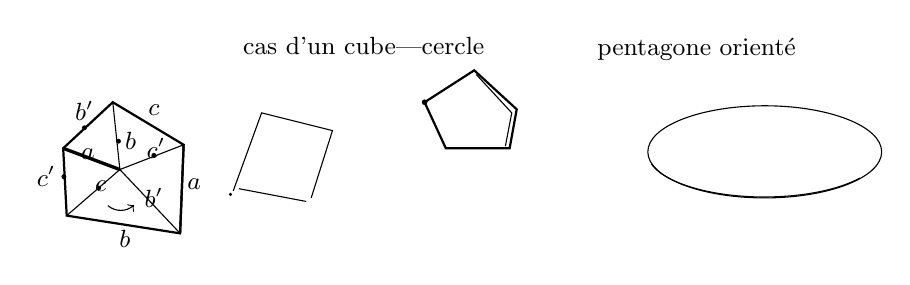
\begin{tikzpicture}[scale=.9,every node/.style={font=\small}]
\node[anchor=west]at(3,2.25){cas d'un \unsure{cube|cercle}};
\node[anchor=west]at(8,2.2){pentagone orienté};
\begin{scope}[shift={(1.4,.6)}]
\draw[thick](-.8,.2)--(-.1,.85)--(.9,.25)--(.85,-1)--(-.75,-.75)--cycle;
\draw[very thick](-.8,.2)--(0,-.1);\draw[thick](.9,.25)--(.85,-1);
\draw(-.1,.85)--(0,-.1)--(.85,-1);\draw(-.75,-.75)--(0,-.1)--(.9,.25);
\foreach\p in{(-.5,.49),(-.79,-.2),(-.02,.3),(-.3,-.36),(.48,.1)}\fill\p circle(.035);
\draw[->](-.17,-.61)to[bend right=40](.2,-.6);
\node at(-.5,.73){$b'$};\node at(.48,.74){$c$};\node at(-.45,.12){$a$};\node at(.15,.3){$b$};\node at(.51,.2){$c'$};\node at(-1.04,-.2){$c'$};\node at(-.27,-.34){$\unsure{c}$};\node at(.48,-.5){$b'$};\node at(1.05,-.3){$a$};\node at(.07,-1.08){$b$};
\end{scope}
\draw[thin](3,.2)--(3.4,1.3)--(4.4,1.05)--(4.1,.1);\draw[thin](3.08,.23)--(4.03,.05);\fill(2.96,.15)circle(.025);
\draw[thick](6,.8)--(5.7,1.45)--(6.4,1.9)--(7,1.35)--(6.9,.8)--cycle;
\draw[thin](6.43,1.84)--(6.93,1.3)--(6.84,.83);\fill(5.7,1.45)circle(.04);
\draw(10.5,.75)ellipse(1.65 and .65);\draw[thin](8.9,.58)arc(195:325:1.65 and .63);
\end{tikzpicture}}

\figure{\begin{tikzpicture}
\node[rotate=180,inner sep=0pt] {\begin{minipage}{13.8cm}\footnotesize
\begin{tabular}{l@{\hspace{1.5cm}}l}
U N I V E R S I T E&MONTPELLIER, le 31 MAI 1979\\
DES SCIENCES ET TECHNIQUES&\\
DU LANGUEDOC&\\
------------&\\
Service de la Scolarité&\\
MR / GJ&\\
Diffusion : Liste A&\\
N\textsuperscript{o} : 3161&
\end{tabular}

\begin{center}
\uline{AVIS DE SOUTENANCE D'UNE THESE DE DOCTORAT D'UNIVERSITE}\\[5pt]
\uline{( SCIENCES\quad NATURELLES )}
\end{center}

\uline{Nom et prénom du candidat} : B E Y R I E S\quad A n d r é

\uline{Titre de la thèse} : Le greffage, moyen de lutte contre les parasites telluriques des Solanées cultivées pour leurs fruits.

\uline{Date, heure et lieu de soutenance prévus:}
\begin{center}20 JUIN 1979 à 10 Heures\\Salle de cours n\textsuperscript{o} 5\end{center}

\uline{Nom du Directeur de thèse} :
\begin{center}Monsieur le Professeur VAGO.\end{center}

\uline{Désignation du laboratoire où la thèse est préparée} :

Laboratoire de Recherches de la Chaire de Biologie et Pathologie Végétales ENSA et INRA - Montpellier .

\uline{Résumé de la thèse} :

\hspace*{2cm}L'objectif de ce travail, commencé en 1963, est consacré à la mise au point d'une méthode de lutte contre les parasites du sol de la Tomate, de l'Aubergine et du Piment dans des conditions climatiques différentes : méditerra-\\néenne et tropicale.

\hspace*{2cm}Le greffage de variétés sensibles sur des porte-greffes résistant à un ou plusieurs parasites telluriques permet de lutter efficacement contre ces derniers en cultures intensives pratiquées sur de petites exploitations.

\uline{Durée approximative des recherches ayant abouti à la thèse} : 15 ans.

\uline{Composition du jury proposé} :\\
\hspace*{3cm}MM.:\\
\hspace*{3.5cm}\begin{tabular}{ll}VAGO&C.\\PARIS&N.\\BOUIX&G.\\MESSIAEN&C.M.\end{tabular}

\begin{flushright}Le Secrétaire Général,\\[4pt]
\begin{tikzpicture}[scale=.7]\node at(0,0){\unsure{E. Siau}};\draw(-2,-.5)to[bend left=18](1.4,.28)to[bend left=12](-2,-.5);\draw(-1.9,-.6)--(1.35,.44);\draw(.4,-.58)to[bend right=12](.55,.32)to[bend left=20](.7,-.5);\end{tikzpicture}\\
\uline{E. S I A U}
\end{flushright}
\end{minipage}};
\end{tikzpicture}}
\mspage{65}

\scanpage{67}
\[
-1-(-1)\;/\;0\;/\;1\mathrel{\vert\!\!-}0
\qquad -\frac{1}{4i}(i-1)^2=\frac12
\]
\diagram{\begin{tikzcd}[ampersand replacement=\&, column sep=large]
X_2\arrow[r,no head,"z\mapsto z^2"]\&X_1\arrow[r]\&X_0
\end{tikzcd}}
\[
\begin{array}{ccc}
0&0\mid\infty&\infty\\
1\quad-1&1&0\\
\infty&\deleted{\unsure{-1|\infty}}&1
\end{array}
\qquad\unsure{\text{en}|i}\quad -1+1-2i
\]
\figure{\begin{tikzpicture}[scale=.76, every node/.style={font=\small}]
\begin{scope}[rotate=180,transform shape]
\node[anchor=west]at(0,0){Cartes};\node[anchor=west]at(0,-.7){Cartes orientées};
\node[anchor=west]at(3.3,0){$\unsure{\mathcal G_2|\Gamma_2}$-ens};\node[anchor=west]at(3.3,-.7){$\unsure{\mathcal G_2^0|\Gamma_2^0}$-ens};
\node[anchor=west]at(6.8,0){$\sigma_0^2=\sigma_1^2=\sigma_\infty^2=(\sigma_0\sigma_\infty)^2=1$};
\node[anchor=west,align=left]at(6.8,-.9){$\bigl(\unsure{\rho_0,\rho_1,\rho_\infty|f_0,f_1,f_\infty},$\\$\qquad\unsure{\rho_0\rho_1\rho_\infty=\rho_1^2|f_0f_1f_\infty=f_1^2}=1\bigr)$};
\node[anchor=west]at(3.4,-2.05){$\varphi(z)=\dfrac{z-1}{z+1}$};
\node[anchor=west]at(-.1,-2.1){$\begin{array}{ccc}0&\longrightarrow&1\\1&\mathrel{-}&1\end{array}$};
\node[anchor=west]at(-.15,-3.15){$i,$};
\node[anchor=west]at(.2,-4.05){$\begin{array}{ccc}1&\mathrel{-}&1\\-1&\mathrel{-}&0\\0&\mathrel{-}&\infty\end{array}$};
\node at(2.3,-3.18){$\deleted{\unsure{z}}$};\node at(3.35,-3.8){$\deleted{\unsure{i}}$};
\node[anchor=west]at(3,-4.18){$i,-i\longmapsto\tfrac12$};\node at(3.6,-4.9){$z$};
\node[anchor=west]at(4.7,-5.45){$(0,\infty)$};\node at(5.45,-6.15){$1$};\node at(5.45,-6.8){$0$};
\node at(8,-5.15){$\left(\dfrac{z-1}{z+1}\right)^2$};
\begin{scope}[shift={(8.1,-3.35)}]
\draw(-1.25,0)arc(180:0:1.25 and .95);\draw(-1.25,-.15)arc(180:360:1.25 and .95);\draw(-1.35,-.05)--(1.3,-.05);
\fill(0,-.05)circle(.035);\node[below]at(0,-.06){$0$};\node[left]at(-1.35,-.1){$\unsure{\beta|3}$};\draw(1.3,-.1)--(1.45,-.1);
\end{scope}
\begin{scope}[shift={(-3,-1.9)}]
\draw(-.7,-.5)--(-.75,.4)--(0,.65)--(.7,.38)--(.35,-.5)--cycle;
\draw(-.7,-.5)--(0,.65)--(.35,-.5);\draw(-.7,-.22)--(-.45,.02)--(-.67,.06)--(-.41,.21);\draw(.24,.55)--(.42,.32)--(.47,.49)--(.58,.3)--(.6,.45);
\draw(0,.7)--(.2,1.55);\node at(.25,.97){$0$};\node[below]at(-.7,-.5){$1$};\node[below]at(.35,-.5){$\infty$};
\end{scope}
\begin{scope}[shift={(-3.1,-4.25)}]
\draw(-1,0)arc(180:0:1 and .6);\draw(-1,-.12)arc(180:360:1 and .6);\draw[thick](-1,-.02)--(-.15,-.06);\draw[thick](.15,-.09)--(1.03,-.12);
\fill(-.05,-.07)circle(.025);\node[above]at(-.05,-.08){$0$};\node at(0,.3){$r$};\node at(0,-.4){$\sigma_0r=\sigma_1r$};\node[left]at(-1.06,0){$1$};\node at(-1.2,-.25){$\unsure{\varphi}$};\node[right]at(1.02,-.1){$\infty$};
\end{scope}
\begin{scope}[shift={(-2.4,-7.35)}]
\draw(0,0)circle(1.25);\draw[dashed](-1.17,.3)--(-.1,.2);\fill(-.1,.2)circle(.03);\node[right]at(-.1,.2){$0$};
\draw[thick](-1.15,.25)to[bend right=45](-.25,-.4);
\end{scope}
\draw[very thick](1.35,-6.65)--(3.25,-6.7);\fill(1.35,-6.65)circle(.045);\fill(3.25,-6.7)circle(.045);\node[below]at(1.35,-6.65){$0$};\node[below]at(3.25,-6.7){$1$};
\begin{scope}[shift={(2,-9.4)}]
\draw(0,0)circle(1.48);\draw[dashed](-1.46,.05)arc(180:0:1.46 and .27);\draw(-1.46,.05)arc(180:360:1.46 and .27);
\draw[very thick](-.63,-.18)to[bend right=6](.65,-.19);\fill(-.63,-.18)circle(.075);\fill(.65,-.19)circle(.075);\node[below]at(-.63,-.18){$0$};\node[below]at(.65,-.19){$0$};\node at(0,-.05){$1$};\fill(.07,.3)circle(.035);\node[right]at(.07,.3){$\infty$};
\draw[->](-.05,1.05)--(-.08,1.26)--(-.4,1.06);\node[right]at(.1,1.12){$1\quad-1\quad0.$};
\end{scope}
\begin{scope}[shift={(-1,-12.5)}]
\draw(0,0)ellipse(2 and .8);\draw[very thick](-1.55,-.5)to[bend right=12](.2,-.79);\fill(.2,-.79)circle(.075);\fill(-1.55,-.5)circle(.03);\node[below]at(-1.55,-.5){$1$};\fill(.53,.77)circle(.03);\node[above]at(.53,.77){$\infty$};
\end{scope}
\node at(5.5,-12.75){$\dfrac{\left(\dfrac{z-1}{z+1}\right)^2}{\left(\dfrac{z-1}{z+1}\right)^2-1}$};
\node[align=left]at(8.6,-13.1){$=\dfrac{(z-1)^2}{(z-1)^2-(z+1)^2}$\\[10pt]$=\dfrac{(z-1)^2}{-4z}$};
\draw[thin](-.1,.65)to[bend right=5](-1.7,-9.2)to[bend right=5](-1.9,-14.8);
\draw[thin](7.2,-1.25)to[bend right=6](6.2,-8.8)to[bend right=5](6,-15.4);
\end{scope}
\end{tikzpicture}}
\diagram{\begin{tikzcd}[ampersand replacement=\&, column sep=large]
X_1\arrow[r]\&\mathbb X_1\arrow[r,"z\mapsto z^2"]\&\mathbb X_0\arrow[r,no head,"\psi"]\&\mathbb X_0
\end{tikzcd}}
\[
(0,1,\infty)\longrightarrow(0,1,\infty)\mathrel{\vert\!\!-}\quad0\quad\infty\quad1
\]
\mspage{66}

\scanpage{68}
\diagram{\begin{tikzcd}[ampersand replacement=\&, column sep=large,row sep=large]
M_{0,5}\arrow[r,hook]\arrow[dr,bend right=25,hook]\&\widehat M_{0,5}\\
\&\widehat M'_{0,5}\arrow[u,bend right=25,hook]\arrow[d,no head,"\simeq"']\\
\&\widehat{\mathcal X}_{0,4}^{*}
\end{tikzcd}}
--- correspond. aux courbes MD de type $(0,5)$ qui restent stables en \deleted{\unsure{le}} abandonnant le trou $5$
\deleted{$\unsure{\ell}$}

\diagram{\begin{tikzcd}[ampersand replacement=\&, column sep=large]
\widehat{\mathcal X}_{0,4}\arrow[r]\&\mathbb P^1\times\mathbb P^1
\end{tikzcd}}
éclatement de trois points de la diagonale $\Delta$, correspondant aux pts $0,1,\infty$
\figure{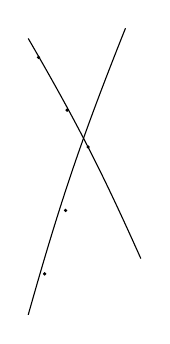
\begin{tikzpicture}[scale=.65]
\draw[thin](-1,2.2)to[bend left=3](1.2,-2.1);\draw[thin](.9,2.4)to[bend right=3](-1,-3.2);
\foreach\p in{(-.8,1.83),(-.24,.8),(.17,.08),(-.27,-1.16),(-.68,-2.4)}\fill\p circle(.035);
\end{tikzpicture}}
\[
\widehat{\mathcal X}_{0,4}^{*}\simeq\deleted{\unsure{\mathbb P^1\times\mathbb P^1}}\unsure{\mathrel{-}}\widehat{\mathcal X}_{0,4}
-\text{les quatre sections }\widetilde\Delta_{\unsure{0|1}}\quad\widetilde\Delta_{\unsure{2|1}}\quad\widetilde\Delta_{\unsure{\infty|3}},\quad\widetilde\Delta
\]
\[
\deleted{\unsure{\widehat{\mathcal X}_{0,\ell}}}\quad\widehat M_{0,5}\quad\text{via}\quad\widehat{\mathcal X}_{0,4}^{*}\ ?
\]
que manque-t-il :

Courbes \inserted{MD} de type $(0,5)$ qui ne sont plus stables en enlevant un des pts à l'infini
\inserted{Il faut que ce soit une \unsure{courbe régulière}}
\figure{\begin{tikzpicture}[scale=.88,every node/.style={font=\small}]
\node at(-.25,.65){$5$};\draw(0,0)--(1.5,0);\draw(0,0)--(-.16,.9);\draw(0,0)--(.2,.9);\draw(1.5,0)--(1.3,.9);\draw(1.5,0)--(1.55,.9);\draw(1.5,0)--(1.9,.8);
\begin{scope}[shift={(1.5,-2.15)}]
\draw(-1,1.65)to[bend right=5](.95,-.6);\draw(.65,1.5)to[bend left=2](-.55,-2.1);
\draw(-.87,1.43)--(-.67,1.27);\draw(-.85,1.26)--(-.67,1.44);
\node[left]at(-.86,1.31){$5$};\fill(-.52,1.03)circle(.04);\node[left]at(-.52,1.03){$i$};
\foreach\p in{(-.22,-1.09),(-.39,-1.57),(-.49,-1.87)}\fill\p circle(.04);
\node at(-1.55,-.2){$1\leq i\leq4$};
\end{scope}
\begin{scope}[shift={(4.7,-1.9)}]
\draw(0,0)--(1.5,.1)--(2.8,.28);\draw(0,0)--(-.18,1.2);\draw(0,0)--(.3,1.25);\draw(1.5,.1)--(1.47,1.25);\draw(2.8,.28)--(2.58,1.5);\draw(2.8,.28)--(3.3,1.5);
\end{scope}
\node at(10,-2.15){$\mathbb P$};
\begin{scope}[shift={(5.6,-4.45)}]
\draw(-1.3,1.65)--(-.28,-.5);\draw(2.9,1.95)to[bend right=3](2.35,-.7);\draw(-1.15,0)to[bend left=4](3.4,.4);
\foreach\p in{(-1.04,1.12),(-.82,.65),(2.82,1.62),(2.7,1.16),(1.08,.22)}\fill\p circle(.04);
\end{scope}
\end{tikzpicture}}
\deleted{$\unsure{\widehat{\mathcal X}}$}
\diagram{\begin{tikzcd}[ampersand replacement=\&, column sep=large,row sep=large]
\widehat X_{0,4}\arrow[d]\&\widehat{\mathcal X}_{0,4}\times\widehat X_{0,4}\arrow[l]\arrow[d,shift right=1]\phantom{.}\\
\deleted{\widehat M_{0,4}}\arrow[r,phantom,"\supset"]\&\widehat{\mathcal X}_{0,4}\arrow[u,bend right=35,"{\sigma_i\ (1\leq i\leq4),\ \delta}"']
\end{tikzcd}}
\figure{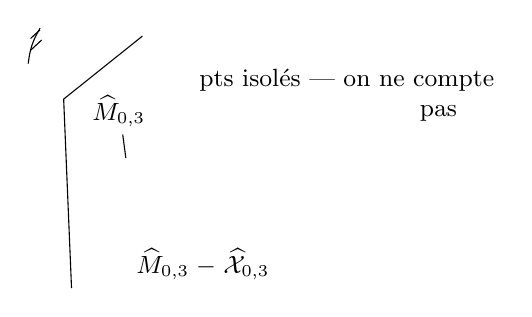
\begin{tikzpicture}[every node/.style={font=\small}]
\draw(-1.2,1.7)--(-2.2,.9)--(-2.1,-1.5);
\node at(-1.5,.75){$\deleted{\widehat M_{0,3}}$};\draw(-1.45,.45)--(-1.41,.15);
\node[anchor=west]at(-1.4,-1.2){$\widehat M_{0,3}\mathrel{-}\widehat{\mathcal X}_{0,3}$};
\node[anchor=west,align=left]at(-.6,.95){\uline{pts isolés} --- on ne compte\\\hspace*{2.8cm}pas};
\draw(-2.5,1.8)to[bend right=12](-2.65,1.35);\draw(-2.62,1.67)--(-2.5,1.78);\draw(-2.62,1.52)--(-2.48,1.65);
\end{tikzpicture}}
\mspage{67}

\scanpage{69}
\figure{\begin{tikzpicture}
\node[rotate=180,inner sep=0pt]{\begin{minipage}{14cm}\small
\begin{tabular}{l@{\hspace{.8cm}}l}
UNIVERSITÉ DES SCIENCES&\\
ET TECHNIQUES DU LANGUEDOC&ACADÉMIE DE MONTPELLIER\\
MONTPELLIER II&\\
Place Eugène Bataillon&\\
34060 MONTPELLIER CEDEX&
\end{tabular}

Tél. : 63.91.44 -- Télex : USTMONT 49944 F

\begin{tabular}{l@{\hspace{3cm}}l}
FA/RR&Montpellier, le\quad\unsure{16|06} FEVR. 1979\quad19
\end{tabular}

01011
\begin{flushright}
Le PRESIDENT de l'UNIVERSITE\\
à\hspace*{5cm}\\
Monsieur le Professeur MICALI\\
Directeur de l'U.E.R. 5
\end{flushright}
\vspace{1cm}
Monsieur le Directeur et Cher Collègue,

\hspace*{1.2cm}Le Bureau du Conseil scientifique dans sa réunion du 8 Février 1979 a réexaminé votre demande de subvention pour l'a-\\ménagement de la bibliothèque de mathématiques.

\hspace*{1.2cm}Il semble difficile d'accorder des crédits sur le bud-\\get ``recherche'' pour couvrir des frais d'aménagement de locaux. En conséquence, il a été envisagé de vous accorder une avance de 50.000 F. Pour vous permettre de rembourser cette somme, le bureau étudiera la possibilité de revaloriser les ``points chercheurs'' at-\\tribués aux mathématiciens.

\hspace*{1.2cm}Je vous signale toutefois que cette avance ne pourra être mise à votre disposition que dans la mesure où la procédure compta-\\ble à utiliser aura été définie et qu'elle vous aura été notifiée.

\hspace*{1.2cm}Veuillez agréer, Monsieur le Directeur et Cher Collègue, l'expression de mes sentiments les meilleurs.

\begin{flushright}
Le Président :\\[4pt]
\begin{tikzpicture}[scale=.6]
\node[font=\itshape]at(0,0){\unsure{L. Thaler}};
\draw(-1.7,.25)to[bend right=65](-1.43,-.23);\draw(-.8,.38)to[bend right=35](-.4,.35)--(-.5,-.32);\draw(-.1,.21)to[bend right=60](.3,-.18)to[bend right=30](.6,.14)to[bend right=45](1,-.18)to[bend right=20](1.6,-.2);
\end{tikzpicture}\\
L. THALER\\[3pt]
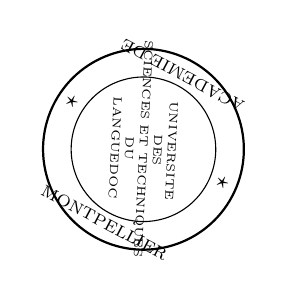
\begin{tikzpicture}[scale=.85,rotate=-28,transform shape]
\draw[thick](0,0)circle(1.5);\draw(0,0)circle(1.08);
\node[font=\scriptsize,rotate=180]at(0,1.25){\unsure{ACADEMIE DE}};
\node[font=\scriptsize]at(0,-1.24){MONTPELLIER};\node at(-1.28,.13){$\star$};\node at(1.27,.12){$\star$};
\node[font=\tiny,align=center,rotate=-65]at(0,0){UNIVERSITE\\\unsure{DES}\\SCIENCES \unsure{ET TEC}HNIQUES\\DU\\LANGUEDOC};
\end{tikzpicture}
\end{flushright}
\end{minipage}};
\end{tikzpicture}}
\mspage{68}

\scanpage{71}
\[
\bigotimes_{i\in K}L_i=L_K
\]
\deleted{$\unsure{A}$}
\figure{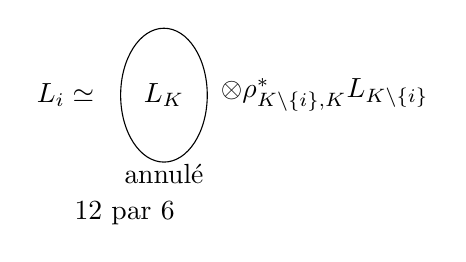
\begin{tikzpicture}[every node/.style={font=\normalsize}]
\node at(0,0){$L_i\simeq$};\node at(1.25,0){$\uline{L_K}$};\draw(1.25,0)ellipse(.55 and .85);
\node[anchor=west]at(1.85,0){$\otimes\rho_{K\setminus\{i\},K}^{*}L_{K\setminus\{i\}}$};
\node at(1.25,-1){annulé};\node at(.75,-1.5){\deleted{$12$ \unsure{par} $6$}};
\end{tikzpicture}}
\diagram{\begin{array}{l|c|c|c}
n&4&5&6\\\hline
(n-1)(n-2)&6&12&20\\\hline
\begin{gathered}\text{meilleur}\\\text{\unsure{exposant}}\\\text{pour trivialiser}\\L\end{gathered}&3&12?&20?\\\hline
\begin{gathered}\text{meilleur}\\\text{\unsure{exp.} pour}\\\text{trivialiser }L_i\end{gathered}&6&12?&60?\\\hline
\begin{gathered}\text{exposant}\\\text{pour}\\\text{trivialiser}\\\uuline{H^1(M_{0,I},\mathfrak S_I;\mathbb G_m)}\end{gathered}&&&\\\hline
\begin{gathered}\text{\unsure{diviseurs}}\\H^1(M_{0,I},\mathfrak S_{I\setminus\{i\}};\mathbb G_m)\end{gathered}&&&\\\hline
\end{array}}
\figure{\begin{tikzpicture}\draw(0,0)--(2,.9);\end{tikzpicture}}
\[
L_K\qquad\text{cas }n=5
\]
\[
\unsure{\simeq}\prod_{A\in\mathcal P_4}\rho_A^*(\uline{L_A})
\]
\inserted{annulé par $3$}
\[
=\prod_{\substack{\unsure{(i,A)|(i\in A)}\\i\in A\in\mathcal P_4(K)}}L_i
=\left(\prod_{i\in K}L_i\right)^{\otimes4}
=L^4
\]
\[
(L^4)^3\simeq\mathcal O
\]
\deleted{\unsure{annulé par}}

\figure{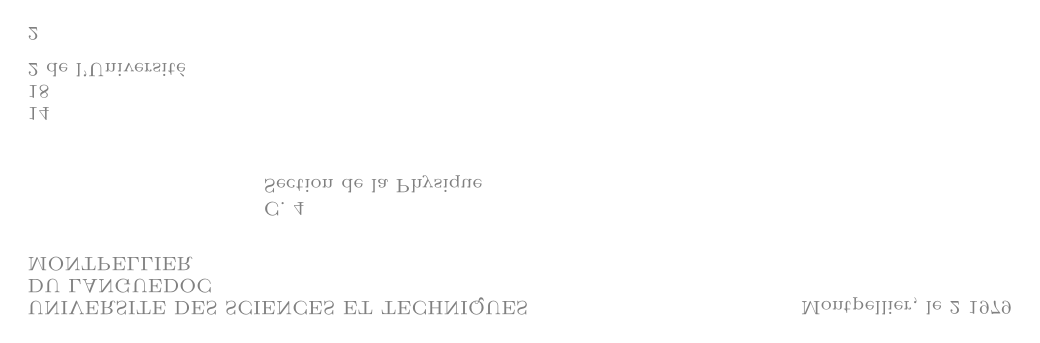
\begin{tikzpicture}
\node[yscale=-1,transform shape,text=gray,inner sep=0pt]{\begin{minipage}{12.5cm}\scriptsize
\unsure{UNIVERSITE DES SCIENCES ET TECHNIQUES}\hfill\unsure{Montpellier, le}\ \illegible{2}\ \unsure{1979}\\
\unsure{DU LANGUEDOC}\\
\uline{\unsure{MONTPELLIER}}\\[12pt]
\hspace*{3cm}\unsure{C.}\ \illegible{4}\\
\hspace*{3cm}\uline{\unsure{Section de la Physique}}\\[18pt]
\illegible{14}\\
\illegible{18}\\
\illegible{2}\ \unsure{de l'Université}\\[5pt]
\illegible{2}
\end{minipage}};
\end{tikzpicture}}
\mspage{70}

\scanpage{72}
\figure{\begin{tikzpicture}[every node/.style={text=gray}]
\node[xscale=-1,transform shape]at(0,0){$\unsure{3}\ \unsure{=|-}\ \unsure{L_K}$};
\node at(-.1,-.65){$\unsure{r}$};
\end{tikzpicture}}
\figure{\begin{tikzpicture}
\node[rotate=180,transform shape,inner sep=0pt]{\begin{minipage}{15cm}\ttfamily
\begin{tabular}{ll}
UNIVERSITE DES SCIENCES \& TECHNIQUES&Session de Juin 1978\\
\hspace*{2cm}DU LANGUEDOC&\\
\hspace*{2cm}\uline{Mathématiques}&
\end{tabular}
\par\vspace{1.1cm}
\begin{center}C4 Math. Pures et Approfondies,\\[12pt]
\uline{Option de M. Petrich}\end{center}
\vspace{1.1cm}
\hspace*{1.2cm}Décrire les classes de conjugaison de sous-groupes et d'éléments

du groupe alterné $\unsure{G_5|\mathcal G_5}$, en indiquant leur interprétation géométrique en

termes de l'icosaèdre.
\hfill\raisebox{1.5\baselineskip}{-}
\par\vspace{1cm}
\begin{center}\begin{tikzpicture}\draw(0,0)--(1.3,0);\end{tikzpicture}\end{center}
\end{minipage}};
\end{tikzpicture}}
\mspage{71}

\scanpage{73}
\begin{tabular}{ll}
UNIVERSITE DES SCIENCES \& TECHNIQUES&Session de Juin 1978\\
\hspace*{2cm}DU LANGUEDOC&\\
\hspace*{2cm}\uline{Mathématiques}&
\end{tabular}

\begin{center}C4 Math. Pures et Approfondies,\\[12pt]
\uline{Option de M. Petrich}\end{center}

Décrire les classes de conjugaison de sous-groupes et d'éléments du groupe alterné $\unsure{G_5|\mathcal G_5}$, en indiquant leur interprétation géométrique en termes de l'icosaèdre.
\margin{-}
\figure{\begin{tikzpicture}\draw(0,0)--(1.3,0);\end{tikzpicture}}

\[
\zeta_A\in\Gamma(M_{0,I},L_A^*)
\]
\[
\prod_A\zeta_A\in\Gamma(M_{0,I},\bigotimes_A L_A)
\]
\figure{\begin{tikzpicture}\fill(0,0)circle(.035);\fill(.8,-.05)circle(.035);\fill(1.25,-.05)circle(.035);\end{tikzpicture}}
\deleted{$\unsure{\zeta}$}
\[
A\in\mathcal P_3(I)
\]
\figure{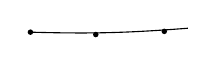
\begin{tikzpicture}\draw(0,0)to[bend right=3](2,0.05);\fill(0,0)circle(.035);\fill(.83,-.03)circle(.035);\fill(1.7,.01)circle(.035);\end{tikzpicture}}
\deleted{$\unsure{4|\ast}$}
\diagram{\begin{tikzcd}[ampersand replacement=\&]
M_{0,I}\arrow[r]\&M_{0 A}
\end{tikzcd}}
\margin{$i$}
\inserted{$\deleted{\unsure{2}}\ \frac{(n-1)(n-2)}{\deleted{\unsure{2}}\inserted{2}}=\nu$}
\[
\zeta=\prod\zeta_A\in L^{\otimes\deleted{\unsure{2\nu|4\nu}}}
\]
\[
L
\]
\diagram{\begin{tikzcd}[ampersand replacement=\&,column sep=large]
L_i\arrow[r,"{\varphi_{i,A,\omega}}"]\&\mathcal O
\end{tikzcd}}
\[
i\in A\in\mathcal P_3(I)
\]
\[
L=\deleted{\unsure{\prod}}\bigotimes_{i\in I}L_i
\]
\diagram{\begin{tikzcd}[ampersand replacement=\&,column sep=large]
L_i^2\arrow[r,no head,"{\psi_{i,A}}","\simeq"']\&\mathcal O
\end{tikzcd}}
\[
\nu=\frac{\unsure{(n-1)(n-1)|(n-1)(n-2)}}{\unsure{2}}
\]
\diagram{\begin{tikzcd}[ampersand replacement=\&,column sep=large]
\deleted{L_i}\arrow[r,no head,"{\deleted{\unsure{\varphi}}}","{\deleted{\simeq}}"']\&\deleted{\mathcal O}
\end{tikzcd}}
\[
\zeta\in L_i\qquad-\zeta
\]
\[
\zeta_{i,A}^{\deleted{\unsure{*}}}\in\Gamma L_i^2
\qquad\deleted{\unsure{L_2}}\qquad A
\]
\[
\zeta\in L_A^2\ \unsure{\sim}
\]
\figure{\begin{tikzpicture}\draw(0,0)to[out=-90,in=100](.05,-2.1)to[out=-80,in=140](.5,-2.7);\end{tikzpicture}}
\uline{Ex}\quad$n=4,\quad\nu=3$

on \unsure{trouve}\quad$L^{\otimes6}\simeq1$

\uline{Ex}\quad$n=5,\quad\nu=6,$\quad on \unsure{trouve}
\[
L^{\otimes\unsure{6|\sigma}}\simeq1
\]
\[
L_i\simeq L\otimes L_{\uline{I\setminus\{i\}}}^{-1}\simeq L\otimes p_i^*(\mathcal O(\unsure{1|{-1}}))
\]
\diagram{\begin{tikzcd}[ampersand replacement=\&,column sep=large]
p_i:\ M_{0,I}\arrow[r]\&M_{0,I\setminus\{i\}}\simeq\overline\Sigma
\end{tikzcd}}
\mspage{72}

\scanpage{74}
\[\unsure{S_i}\mathcal T_{0,I}\qquad \mathcal T_{0,I}\qquad i_0\ \uline{I}\qquad i'_1\ne i'_0\]
\[i_0\deleted{\unsure{i}}\in I\setminus\{i_1\}
= i_0\amalg\unsure{(I\setminus\{i_0,i_1\})}\]
\[\deleted{\unsure{\pi^2}}\]
\diagram{\begin{tikzcd}[ampersand replacement=\&]\mathcal T_{0,I}\arrow[d,"\unsure{\pi_1}"]\\\mathcal T_{0,I\setminus\{i_1\}}\end{tikzcd}}
\figure{\begin{tikzpicture}\draw (0,0)--(.7,1.6);\end{tikzpicture}}
\diagram{\begin{tikzcd}[ampersand replacement=\&]M_{0,K}\arrow[d]\\M_{0,I}\end{tikzcd}}
\[\unsure{\mathcal T}\qquad \times\quad 1\ 2\ 3\ 4\qquad 5\]
\[H\qquad \unsure{\mathcal O(}\qquad
\mathcal O(4)^{\unsure{\otimes}}\,\deleted{\uline{\unsure{degrés}}}\simeq\mathcal O(-2)\simeq\Omega^1\]
\[\prod_{i\in I}\deleted{\unsure{\mathcal O}}L_i\]
\[H^1(\widetilde G_5,M^!_{0,5};G_m).\qquad
M_{0,I}\hookrightarrow\prod_{i\in\deleted{K}}\uline{\Sigma_{J(i)}}\qquad I\setminus\{i\}\]
\[H^1(M_{0,5};G_m)\simeq 0\]
\[H^0(M^!_{0,5},G_m)\qquad \uline{M_{0,5}}\]
\unsure{à coups d'éclatements}

\[H^2(\mathcal T^+_{0,5},\mathbb Z)=\qquad :\ \text{\unsure{partir de}}\quad\mathbb P_1\times\mathbb P_1\]
\[\unsure{H^1(M^!_{0,5}}\]
\figure{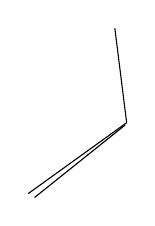
\begin{tikzpicture}\draw (1.1,2.1)--(1.25,.9)--(0,0);\draw (1.23,.87)--(.08,-.05);\end{tikzpicture}}
\diagram{\begin{tikzcd}[ampersand replacement=\&]M^!_{0,5}\arrow[d]\&\unsure{-}\&U_{0,3}\times U_{0,3}\arrow[d]\\M^!_{0,4}\simeq U_{0,3}\&\&U_{0,3}\end{tikzcd}}
\[H^0(U_{0,3},G_m)\qquad\unsure{21}\qquad\unsure{\ne}\]
\figure{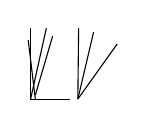
\begin{tikzpicture}\draw (0,.9)--(0,0)--(.5,0);\draw (0,0)--(.2,.9);\draw (.06,0)--(-.03,.75);\draw (.06,.05)--(.28,.8);\draw (.6,0)--(.61,.9);\draw (.6,0)--(.8,.85);\draw (.6,0)--(1.1,.7);\end{tikzpicture}}
\diagram{\begin{tikzcd}[ampersand replacement=\&, column sep=small]0\arrow[r]\&G_m\arrow[r]\&H^0(M^{\unsure{\partial}}_{0,\deleted{K}},G_m)\arrow[r]\&(\mathbb Z^{P_3(K)})'\arrow[r,dash]\&0\end{tikzcd}}
\diagram{\begin{tikzcd}[ampersand replacement=\&, column sep=small]
0\arrow[r,dash]\&\underbrace{H^1(\widetilde G_K,G_m)}_{\unsure{\pm1}}\arrow[r]\&\underbrace{H^1(\widetilde G_K,H^0(M_{0,K},G_m))}_{\unsure{H^1(M_{0,n},\widetilde G_n;G_m)}}\arrow[r]\&H^1(\widetilde G_{\unsure{5}},(\mathbb Z^{P_3(K)})')\arrow[d]\\\&\&\&H^2(\widetilde G_n,\unsure{G_m})
\end{tikzcd}}
\mspage{73}

\scanpage{75}
dont le deuxième est donné par
\[(41)\qquad\boxed{\rho_1\unsure{\leftrightarrow}\sigma_\infty,\ \rho_\infty\longmapsto\rho^{-1},}\quad\rho_0=(\rho_\infty\rho_1)^{-1}\longmapsto\sigma_\infty\rho^{\unsure{\wedge}}=\varepsilon_0\]
et le premier par
\[(42)\qquad\boxed{\tau_{\deleted{\unsure{\infty}}}\longmapsto\tau_\infty},\quad\underset{\underset{\rho_0}{\Vert}}{\tau_{\deleted{\unsure{0}}}}\longmapsto\quad,\quad\boxed{\tau_\infty\longmapsto\tau_{\unsure{a}}}\quad,\]
\figure{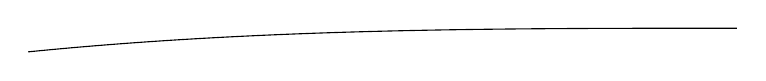
\begin{tikzpicture}\draw (0,0)..controls(3,.3)and(6,.3)..(9,.3);\end{tikzpicture}}
\figure{\begin{tikzpicture}[scale=1.4]
\node at(-.4,1.2){$\unsure{\xi}$};
\draw (0,.3)..controls(.3,.8)and(.7,1.2)..(1.1,1.5)..controls(1.3,1.3)and(1.25,.8)..(1.2,.15);
\draw (0,.3)..controls(.3,.1)and(.8,.1)..(1.15,.15);
\node at(-.1,.13){$0$};\node at(1.3,1.6){$\infty$};\node at(1.3,0){$1$};\node at(-.2,-.6){$\unsure{i}$};
\begin{scope}[xshift=3.1cm,yshift=-.2cm]
\draw (0,.4)--(.75,1.25)--(1,.2)--cycle;
\draw (0,.4)--(.64,.62);\draw (.75,1.25)--(.5,.3);\draw (1,.2)--(.32,.82);
\draw[very thick] (.62,.62)--(1.33,.75)--(1.65,.25)--(1.3,-.5)--(.54,-.08)--cycle;
\draw (.57,.65)--(.51,.03);\draw (1.3,-.5)--(1.33,-.57);\draw (1.34,.71)--(1.7,.29)--(1.64,.2);
\fill (0,.4)circle(.035);\fill (.75,1.25)circle(.035);\fill (1,.2)circle(.035);\fill (.64,.62)circle(.035);\fill (.5,.3)circle(.035);\fill (.32,.82)circle(.025);
\draw (.15,.4)--(.21,.49)--(.24,.38)--(.28,.5)--(.32,.4)--(.38,.52)--(.4,.4)--(.46,.52)--(.49,.4)--(.53,.51);
\node at(-.02,.17){$\unsure{0}$};\node at(.9,1.4){$\unsure{\infty}$};\node at(1.05,.03){$1$};
\end{scope}
\end{tikzpicture}}
\[\pi_{D_n},\quad\pi_{\widetilde G^+_4},\quad\pi_{\widetilde G_4},\quad\pi_{\widetilde G^+_5}\quad\unsure{-}\]
\[\pi_X\qquad\pi_X\longrightarrow X\ \text{une cat : \unsure{en excluant les sommets}}\]
\[\deleted{\pi_{\unsure{P_\infty}}}\qquad\pi_{\mathrm{icos}},\quad\pi_{\mathrm{dodéc}},\quad\pi_{\mathrm{tétr.}},\quad\pi_{\mathrm{cube}},\quad\pi_{\mathrm{oct.}},\quad\deleted{\pi_{\unsure{opicos}}}\]
\[\pi_{\unsure{\mathrm{paricos}}},\qquad\pi_P\longrightarrow\text{polygone combinatoire fini}\ldots\]
\mspage{74}

\scanpage{77}
\figure{\begin{tikzpicture}[scale=1.2]
\draw (0,0) ellipse (1 and 1.1);\draw (0,0) ellipse (1 and .26);
\foreach \x/\y/\lab in {-.45/.25/c,.34/.23/b,-.78/-.15/d,.17/-.24/e,.92/0/a}{\draw (\x,\y)ellipse(.1 and .075);\node[above right]at(\x,\y){$\lab$};}
\draw[very thick](.9,0)ellipse(.09 and .1);\draw(.9,-.1)--(.95,.1)--(.86,-.06)--(.94,.04);
\draw (.08,.04)--(.8,-.16)--(.93,0)--cycle;\foreach \x in {.45,.53,.61,.69,.77}{\draw(\x,.02)--(\x+.08,-.12);}
\node at(-1.12,.18){$v$};\node at(-.16,.4){$u$};\node at(-.21,-.4){$w\unsure{\alpha}$};\node at(.55,-.38){$s$};\node at(.87,.32){$t$};
\draw[->](1.2,-.05)..controls(1.6,.1)and(1.4,.3)..(1.15,.28);
\end{tikzpicture}}
\figure{\begin{tikzpicture}[scale=1.2]
\draw (0,0)ellipse(.85 and 1.05);\draw(0,-.18)ellipse(.85 and .24);\draw(-.08,1.05)..controls(-.68,.4)and(-.67,-.2)..(-.5,-.35);\draw(-.08,1.05)..controls(.4,.7)and(.34,.2)..(.32,-.3);
\draw[dashed](-.08,1.05)..controls(-.2,.6)and(-.45,.2)..(-.4,-.06);\draw[dashed](-.08,1.05)..controls(.5,.8)and(.44,.3)..(.3,0);
\foreach\x/\y/\l in {-.08/1.05/a,-.4/-.06/c,.3/0/b,-.5/-.35/d,.32/-.3/e}{\draw(\x,\y)ellipse(.09 and .055);\node[above right]at(\x,\y){$\l$};}
\fill(.77,-.18)circle(.06);\draw(.7,-.17)--(.92,-.18);\draw[->](.95,-.3)..controls(1.18,-.1)and(1.1,.12)..(.94,.05);
\draw(0,.9)--(-.14,.09)--(.18,.1)--cycle;\draw(-.05,.6)--(.07,.26);\draw(-.08,.48)--(.14,.14);\draw(-.12,.27)--(.03,.12);
\end{tikzpicture}}
\figure{\begin{tikzpicture}[scale=1.2]
\draw(0,0)ellipse(.85 and 1);\draw(0,-.12)ellipse(.85 and .3);
\draw(0,1)..controls(-.65,.8)and(-.6,.1)..(-.7,-.2);\draw(0,1)..controls(.45,.5)and(.42,-.7)..(0,-1);\draw[dashed](0,1)..controls(-.5,.6)and(-.5,-.5)..(0,-1);\draw[dashed](0,1)..controls(.4,.8)and(.38,.6)..(.4,.2);
\foreach\x/\y/\l in {0/1/a,-.4/.18/c,.4/.2/b,-.7/-.2/d,.3/-.4/e}{\draw(\x,\y)ellipse(.08 and .055);\node[above right]at(\x,\y){$\l$};}
\node at(.83,-.15){$\times$};\draw(0,.93)--(-.08,.04)--(.24,.11)--cycle;\foreach\y in {.15,.26,.37,.48,.59,.7,.8}{\draw(-.07,\y)--(.23-.22*\y,\y+.045);}
\end{tikzpicture}}
\figure{\begin{tikzpicture}[scale=1.1]
\coordinate(w)at(-2,.7);\coordinate(u)at(.1,1.9);\coordinate(t)at(2.2,1.05);\coordinate(s)at(-.05,.08);\coordinate(x)at(0,1.1);\coordinate(y)at(1.12,.48);
\draw(w)..controls(-2.5,1.7)and(-1,2.2)..(u)..controls(1.5,2)and(2.2,1.6)..(t)..controls(2.3,.2)and(.8,-.05)..(s)..controls(-.9,-.05)and(-1.6,.3)..cycle;
\draw(w)--(-1.3,1.72);\draw(w)--(s)--(t)--(u);\draw[dashed](u)--(x)--(w);\draw[dashed](x)--(t);\draw(x)--(s)--(y)--cycle;
\foreach\a/\b/\c/\d in {.05/.3/.45/.75,.1/.45/.6/.67,.1/.62/.76/.61,.15/.78/.9/.55}{\draw(\a,\b)--(\c,\d);}
\draw[yshift=.04cm](y)..controls(1.6,.4)and(1.8,.7)..(t);\draw[dashed](x)--(1.15,1.02)--(y);\node at(1.1,1.2){$(d)$};\node at(-.28,.72){$(c)$};
\foreach\p in {x,y,s}{\fill(\p)circle(.065);}
\node[below left]at(w){$w$};\node[above]at(-1.3,1.72){$v$};\node[above]at(u){$u$};\node[right]at(t){$t$};\node[below]at(s){$s$};
\foreach\a/\b/\l in {-2.05/1.38/d,-.8/2.02/c,1.72/1.75/b,-1.3/.25/e,1.4/.3/a}{\draw(\a,\b)ellipse(.15 and .09);\node[above]at(\a,\b+.1){$\l$};}
\draw[->](2.5,1.6)..controls(2.6,1.9)..(2.4,2);
\coordinate(p)at(-3.15,-.5);\coordinate(q)at(-2.5,-2.35);\coordinate(r)at(0,-1.72);
\draw(w)--(p)--(q)--(r);\draw(s)--(r)--(2.05,-2.3);\draw(t)--(3.25,-.35);\draw[->](3.25,-.6)--(2.45,-2.2);
\node at(-2.8,.2){$(b)$};\node at(-3.27,-1.5){$(a)$};\node at(-1.6,-2.34){$(d)$};\node at(.25,-.9){$(c)$};\node at(1,-2.32){$(b)$};\node at(2.9,-1.3){$(e)$};\node at(2.9,.4){$(d)$};
\draw(p)--(-1.8,-.86)--(q);\draw(p)--(-1.85,-.73);\foreach\a in {0,.15,.3,.45,.6,.75}{\draw(-3+.8*\a,-.48-.2*\a)--(-2.7+.8*\a,-.35-.7*\a)--(-2.65+.8*\a,-.2-.4*\a);}
\node at(-1.88,-1.22){$(\unsure{g})$};\draw[->](y)--(1.95,-.6);\draw[->](1.95,.6)--(1.95,-.6);\draw[dashed](s)--(1.95,-.6);\draw[dashed](y)--(.82,-.45);\node at(.96,-.42){$\unsure{g}$};\node at(2.16,-.02){$h$};\draw[->](1.56,.19)--(1.92,.23);\draw[->](-2.5,1.4)--(-3.4,-.2)--(p);
\end{tikzpicture}}
\figure{\begin{tikzpicture}
\coordinate(s)at(0,0);\coordinate(t)at(2.7,1.3);\draw(s)..controls(.8,1.25)and(1.8,1.6)..(t)..controls(2.05,.35)and(.7,-.35)..cycle;
\draw(s)--(1.3,.63);\draw[dashed](1.3,.63)--(t);\draw[dashed](.98,1.08)--(1.5,.17);\fill(1.3,.63)circle(.04);\node[right]at(1.3,.63){$\unsure{\alpha}$};
\foreach\x/\a/\b in {.3/.21/.45,.5/.32/.7,.7/.42/.88,.9/.52/1.02,1.1/.57/.94}{\draw(\x,\a)--(\x,\b);}
\node[below left]at(s){$s$};\node[right]at(t){$t$};\node at(.4,.91){$c$};\node at(1.8,1.6){$d$};\node at(2.15,.33){$b$};\node at(.67,-.2){$e$};
\end{tikzpicture}}
\diagram{\begin{tikzcd}[ampersand replacement=\&, column sep=large,row sep=large]
\&\begin{gathered}\unsure{F}\ \text{faces du}\\\text{\unsure{bidodécagone|bidodécaèdre}}\\(12)\end{gathered}\\
\begin{gathered}R\\\text{repères}\\\text{du \uline{\unsure{bidodécagone|bidodécaèdre}}}\\(120)\ \text{\unsure{gauche}}\end{gathered}\arrow[ur]\arrow[r]\arrow[dr]
\&\begin{gathered}A\ \text{arêtes}\ \deleted{\unsure{du}}\\\deleted{\unsure{bi}}\text{dodécagone}\\(30)\end{gathered}\\
\&\begin{gathered}S\ \text{sommets}\\\text{du \unsure{bidodécagone|bidodécaèdre}}\\(20)\end{gathered}
\end{tikzcd}}
\figure{\begin{tikzpicture}[scale=1.2]
\draw(0,0)ellipse(.95 and .95);\draw(0,-.18)ellipse(.95 and .3);\draw(-.2,.95)..controls(.25,.65)and(.2,-.25)..(.2,-.48);\draw(-.2,.95)..controls(-.7,.5)and(-.75,-.1)..(-.65,-.42);\draw[dashed](-.2,.95)..controls(.4,.7)..(.4,.1);
\foreach\x/\y/\l in {-.2/.95/a,-.45/.1/c,.4/.1/b,-.65/-.42/d,.2/-.48/e}{\draw(\x,\y)circle(.065);\node[above]at(\x,\y+.08){$\l$};}
\node at(-.31,-.45){$\times$};\node at(.59,-.33){$s$};\node at(1,-.2){$\alpha$};\draw[->](1.27,-.1)..controls(1.4,.1)and(1.4,.24)..(1.2,.4);\draw[->](-.2,-.95)arc(270:252:.95);
\end{tikzpicture}}
\figure{\begin{tikzpicture}
\draw(0,0)ellipse(1 and .35);\foreach\x/\y/\l in {-.5/.29/c,.58/.28/b,.99/-.03/a,-.6/-.28/d,.56/-.3/e}{\draw(\x,\y)ellipse(.1 and .06);\node[above right]at(\x,\y){$\l$};}
\node at(.91,-.36){$s$};\draw[dashed](-.4,.22)--(-.4,-.28);\draw[dashed](.47,.17)--(.2,-.5);\draw(.56,-.45)--(.2,-1.4);\draw[->](-.65,-.28)..controls(-.57,-.91)..(-.05,-1.34);\draw(.2,-1.4)ellipse(.08 and .055);\draw(-.12,-.92)--(.02,-1.2);\draw(.2,-.84)--(.13,-1.25);\node at(.12,-1.64){$\unsure{,}$};
\end{tikzpicture}}
\figure{\begin{tikzpicture}
\draw(0,0)ellipse(1 and .3);\foreach\x/\y/\l in {-.54/.23/c,.48/.25/b,.98/-.02/a,-.78/-.2/d}{\draw(\x,\y)ellipse(.09 and .055);\node[above right]at(\x,\y){$\l$};}
\draw[very thick](.36,-.29)ellipse(.14 and .08);\draw(.23,-.3)--(.48,-.27)--(.29,-.21)--(.42,-.37);\draw[->](.35,-.22)..controls(.39,.1)and(.25,.6)..(.07,1.02);
\end{tikzpicture}}
\[2\times(6+15+10)=62\]
\mspage{76}

\scanpage{78}
\begin{center}
UNIVERSITE DES SCIENCES ET TECHNIQUES\\
DU LANGUEDOC\\
---\\
U.E.R. 5\\
Place Eugène Bataillon\\
34060 MONTPELLIER CEDEX\\
---
\end{center}
\begin{flushright}Montpellier, le\quad 12 février 1982\end{flushright}
\figure{\begin{tikzpicture}[scale=1.2]
\draw[thick](0,.6)--(1,1.2)--(2.7,1.15)--(3.7,.3)--(3,-.25)--(1.55,.02)..controls(1.4,.2)and(1.42,.6)..(1.3,.7)--(.3,.05)--cycle;
\draw(0,.6)--(-.2,.65)--(.9,1.55)--(2.85,1.48)--(3.7,.3);\draw(-.2,.65)..controls(-.15,.2)..(.15,-.12)--(1.24,.46)..controls(1.35,.1)..(1.4,-.1)--(3,-.37)--(3.7,.19);
\foreach\a/\b/\c/\d in {.35/.38/.5/.65,.9/.6/1.1/1.04,1.35/.75/1.55/1.08,1.68/.35/1.95/1.02,1.95/.14/2.3/.98,2.33/-.08/2.8/.86,2.64/-.18/3.04/.6}{\draw[thin](\a,\b)--(\c,\d);}
\draw(-.35,.65)--(0,.6);\draw(.3,.05)--(.08,-.3);\draw(.9,1.55)--(1,1.9);\draw(1,1.2)--(1,1.6);\draw(2.7,1.15)--(2.9,1.65);\draw(3.7,.3)--(4.2,.35);\draw(3,-.25)--(3,-.8);\draw(1.55,.02)--(1.35,-.3);
\end{tikzpicture}}
\begin{center}\uline{D.E.A. DE MATHEMATIQUES}\end{center}
\begin{center}Organisation des cours pour l'année 1982 - 1983\end{center}
\figure{\begin{tikzpicture}
\draw(.1,.6)--(2.6,.65)--(2.75,.05)--(2.6,-.28)--(0,-.6)--(-.3,-.3)--(-.25,.25)--cycle;
\draw[thick](-.25,.25)--(.4,0)--(1,.1)--(2.3,.14)--(2.6,.65);\draw[thick](-.3,-.3)--(1,.1)--(2.6,-.28);\draw(.1,.6)--(1,.1)--(2.6,.65);\draw(0,-.6)--(1,.1)--(2.6,-.28);\draw(.1,.6)--(.4,0)--(0,-.6);\draw(2.6,.65)--(2.3,.14)--(2.6,-.28);\draw(.1,.6)--(-.2,.98);\draw(0,-.6)--(-.23,-.8);\draw(2.3,.14)--(3.15,.14);\draw(2.6,.65)--(2.88,1);\draw(2.6,-.28)--(2.9,-.55);
\end{tikzpicture}}
\begin{center}------\end{center}
\figure{\begin{tikzpicture}
\draw(0,0)ellipse(.14 and .3);\draw(2,.25)ellipse(.17 and .3);\draw(0,.3)--(2,.55);\draw[thick](.1,0)--(1.85,.24);\draw(0,-.3)--(2,-.05);\draw(0,.3)--(-.45,.8);\draw(0,-.3)--(-.13,-.6);\draw(1.85,.24)--(2.1,.95);\draw(2,.1)--(2.8,.4);\draw(2,-.05)--(2.83,-.5);\draw(1.88,.2)--(2.09,.05)--(1.97,.33);\draw(-.05,.1)--(.08,-.13);\draw[thin](0,.67)..controls(.5,1.1)and(1.2,1.2)..(1.8,1.15);
\end{tikzpicture}}
Réunion le 26 février à 15 h, salle 208

\figure{\begin{tikzpicture}
\draw(0,.45)--(2,.62);\draw(0,-.45)--(2.3,-.26);\draw[thick](0,.45)--(1,.1)--(2.5,-.28);\draw[thick](0,-.45)--(1,.1)--(2.3,.5);\draw(-.2,.3)--(-.36,.17)--(-.36,-.11)--(0,-.45);\draw(2.3,.5)--(2.5,.29)--(2.45,0)--(2.3,-.26);\draw(-.36,.17)--(-.65,.4);\draw(-.36,-.11)--(-.72,-.3);\draw(0,.45)--(-.3,.75);\draw(0,-.45)--(-.23,-.62);\draw(2.3,.5)--(2.6,.8);\draw(2.5,.29)--(2.9,.5);\draw(2.45,0)--(2.86,-.15);\draw(2.3,-.26)--(2.61,-.55);\draw(2,.62)--(2.14,.92);\draw(.43,.02)ellipse(.18 and .055);\draw[thin](1.1,.07)..controls(1.7,.7)and(1.87,-.2)..(1.3,.04);\foreach\x in {1.5,1.7,1.9,2.1}{\draw(\x,-.12)--(\x+.19,.33);}
\end{tikzpicture}}
Présence indispensable de tous les collègues intéressés par le fonctionnement du D.E.A. l'an prochain.

\figure{\begin{tikzpicture}
\draw(0,.45)--(2.6,.75)--(2.8,.38)--(2.78,-.05)--(2.55,-.3)--(0,-.6)--cycle;\draw[thick](0,.45)--(.4,-.05)--(1.35,.05)--(2.2,.1)--(2.6,.75);\draw[thick](0,-.6)--(.4,-.05);\draw[thick](2.2,.1)--(2.8,.38);\draw[thick](2.2,.1)--(2.78,-.05);\draw[thick](2.2,.1)--(2.55,-.3);\draw(0,.45)--(1.35,.05)--(2.55,-.3);\draw(0,-.6)--(1.35,.05)--(2.6,.75);\draw[xshift=-.04cm](0,.45)--(0,-.6);\foreach\x/\y in {0/.45,0/-.6,1.35/.05,2.6/.75,2.8/.38,2.78/-.05,2.55/-.3}{\fill(\x,\y)circle(.028);}
\end{tikzpicture}}
\begin{flushright}P. MOLINO\end{flushright}
\figure{\begin{tikzpicture}[rotate=28]
\draw[thin](0,0)ellipse(2 and 1.15);\draw[thin](0,0)--(.8,1.05);\draw[thick](0,0)--(.3,-1.12);\draw(-.06,-.02)--(.05,.04)--(.02,-.06)--cycle;
\end{tikzpicture}}
\figure{\begin{tikzpicture}
\draw[thick](0,1.4)--(.75,2.2)--(2.2,1.95)--(1.75,1)--(1.1,.8)--(.1,.58)--(-.45,-.18)--(-.2,-.55)--(1.72,-.57)--(2.25,.25)--(1.1,.8)--(0,1.4);
\draw(.1,.58)--(0,1.4);\draw(1.75,1)--(2.25,.25);\draw(-.45,-.18)--(1.1,.8)--(2.2,1.95);\draw(-.2,-.55)--(-.65,-.95);\draw(1.72,-.57)--(2,-.93);\draw(.1,.58)--(-.5,1.15);\draw(1.75,1)--(2.4,1.3);\draw(-.45,-.18)--(-.56,.07);\draw[yshift=.035cm](-.2,-.55)--(.2,-.53)--(.65,-.6)--(1.72,-.57);
\draw[thick](-1.5,-1.35)--(.1,-1.18)--(1.6,-1.05);\draw(-1.5,-1.35)..controls(-1,-1.02)and(-.6,-1.4)..(.1,-1.18)..controls(.6,-.97)and(1.1,-1.15)..(1.6,-1.05)..controls(2,-.94)and(2.3,-.94)..(2.5,-1.08);\foreach\x/\y in {-1.5/-1.35,.1/-1.18,1.6/-1.05}{\draw(\x,\y)circle(.045);}
\end{tikzpicture}}
\figure{\begin{tikzpicture}
\draw(0,0)..controls(-.2,.6)and(.1,1.25)..(.55,1.4)..controls(.75,.65)and(.5,.05)..cycle;\draw(0,0)circle(.045);\draw(.55,1.4)circle(.045);
\end{tikzpicture}}
\figure{\begin{tikzpicture}
\draw[thick](0,1)--(1.1,1.05);\draw(0,1)..controls(.22,.6)..(.36,0)--(1.1,1.05);\draw[thin](.36,0)..controls(.4,.7)..(1.1,1.05);\draw(.36,0)..controls(.6,-.6)and(.8,-.9)..(1,-1.1);\foreach\x/\y in {0/1,1.1/1.05,.36/0}{\draw(\x,\y)ellipse(.07 and .04);}
\end{tikzpicture}}
\mspage{77}

\scanpage{81}
\uline{Lemme} 1\qquad Soit
\[1\longrightarrow L\longrightarrow\widetilde\pi\;\text{---}\;\pi\;\text{---}\;1\]
une suite exacte de groupes, soit $(\unsure{x_i})_{i\in I}$ un syst. de générateurs de $\pi$,
\[(\unsure{a_j})_{j\in J}\qquad\text{\rule{5cm}{.4pt}}\qquad L,\]
$R_\alpha((x_i))=1$ $(\alpha\in A)$ un syst. de relations \unsure{définissantes} de $\pi$, $S_\beta((a_j))=1$ $(\beta\in B)$ un syst. de relations \unsure{définissantes} de $L$. Relevons les $x_i$ en des $\widetilde x_i\in\widetilde\pi$, et choisissons des mots $M_\alpha$ et $M_{i_0j_0}$ $(\alpha\in A,\ \deleted{\unsure{i\in I}}\ (i,j)\in I\times J)$ en \unsure{les} lettres $a_j$, de telle façon qu'on ait
\[
\left\{\begin{aligned}
(1)\quad R_\alpha((\widetilde x_i))&=M_\alpha((a_j))&&\forall\alpha\in A\\
(2)\quad\widetilde x_{i_0}a_{j_0}\widetilde x_{i_0}^{-1}&=M_{i_0j_0}((a_j))&&\forall(i_0,j_0)\in I\times J
\end{aligned}\right.
\]
\margin{relations $\widetilde R_\alpha$ ``\unsure{héritées}'' des rel. de $\pi$}
\margin{relations $\unsure{r_{(i,j)}}$ de ``conjugaison''}
Alors les relations (1) (2), plus les :
\[(3)\qquad\left\{S_\beta((a_j))=1\qquad(\beta\in B)\right.\]
\margin{``relations du \unsure{noyau}'' $S_\beta$}
sont un syst. de relations \unsure{définissantes} pour $\unsure{E|\widetilde\pi})$ p.r. aux générateurs $(\widetilde x_i)$, $(a_j)$.

\uline{NB} Si $L$ est central dans $\unsure{\widehat\pi|\widetilde\pi}$, \deleted{\unsure{les relations}}\inserted{\unsure{il y a}} intérêt à prendre les $M_{i_0j_0}$ les mots vides, donc (2) devient
\[(2')\qquad\widetilde x_i a_j\widetilde x_i^{-1}=a_j\qquad\text{i.e.}\quad[\widetilde x_i,a_j]=1\]
pour $\forall(i,j)\in I\times J$
\mspage{80}

\scanpage{82}
\deleted{
Cas d'un \deleted{\unsure{groupoïde algébrique}}\inserted{hom de groupoïdes}
\diagram{\begin{tikzcd}[ampersand replacement=\&]\widetilde{\mathcal T}\arrow[r,"p"]\&\mathcal T\end{tikzcd}}
qui est surjectif sur les $\pi_0$. On se donne une famille $(\widetilde u_i)_{i\in I}$ de flèches de $\widetilde{\mathcal T}$, \deleted{entre des objets} de projections $u_i$ dans $\mathcal T$ et des relations
\inserted{$\deleted{\unsure{i^{\alpha}}}\ i^{(\alpha)}=(i_0^{(\alpha)},\ldots,\unsure{i_{m_\alpha}^{(\alpha)}})\in I'^{m_\alpha}$}
\[(4)\qquad\unsure{u'_{i^{(\alpha)}_{m_\alpha}}}\,u'_{i^{(\alpha)}_{m_\alpha-1}}\cdots u'_{i^{(\alpha)}_1}u'_{i^{(\alpha)}_0}=1\quad\text{dans }\mathcal T\qquad(\alpha\in A)\]
\inserted{[pour le rôle des relations $R_\alpha$]}
(flèches composables dans $\mathcal T$, avec $\operatorname{or}(u'_{i_0})=\operatorname{ext}(u'_{i_{m-1}})$).
\margin{d'où une famille de flèches $\widetilde u'_{i'}$, $\deleted{\unsure{u_i}}=\widetilde u_i^{\pm1}$ paramétrée par les $i'\in I'\simeq I\times\{\pm1\}$, en posant $\widetilde u'_{(i,\varepsilon)}=\widetilde u_i^\varepsilon$ --- itou pour des $u'_{i'}$}
De plus, on se donne des \deleted{relations}\inserted{flèches} $(a_j)_{j\in J}$ de $\unsure{\mathcal T|\widetilde{\mathcal T}}$ qui sont des
\[\deleted{(5)\qquad\unsure{u}}\]
``flèches fibres'' (leur projection dans $\unsure{\widetilde{\mathcal T}|\mathcal T}$ des identités), \deleted{et des relations}\inserted{d'où des $a'_{j'}=a_j^{\pm1}\quad(j'\in J\times\{\pm1\})$}
\deleted{\unsure{S}} et des relations
\[(5)\qquad a'_{j^{(\beta)}_{n_\beta}}a'_{j^{(\beta)}_{n_\beta-1}}\cdots a'_{j^{(\beta)}_0}=1\]
\[\text{où }j^{(\beta)}=(j^{(\beta)}_0,\ldots,j^{(\beta)}_{n_\beta})\in J'^{\unsure{n_\beta}},\qquad\beta\in B\]
[pour le rôle des rel. $S_\beta$]
\margin{\uline{NB} Les indices \unsure{$i$ sont des éléments de} $\coprod_{n\in\mathbb N^*}I'^n$ \unsure{et $B$ un ens. d'éléments de} $\coprod_{n\in\mathbb N^*}J'^n$}
On suppose

1°) les relations (4) sont une famille \deleted{qui} de relations \unsure{définissantes} pour $\mathcal T$, en \inserted{flèches génératrices $u_i$ $(i\in I)$ et $\operatorname{Ob}\mathcal T$}
(ce qui implique que tous les sommets de $\mathcal T$ sont parmi les origines \inserted{et extr.} des flèches \deleted{\unsure{$u'_{i_j}$ intervenant dans (4)}} (à fortiori $\widetilde{\mathcal T}\text{---}\mathcal T$ est surjectif sur les objets). \deleted{et des}
}
\mspage{81}

\scanpage{83}
Soit $\deleted{\unsure{\widetilde{\mathcal T}\longrightarrow\mathcal T}}$
\[(1)\qquad\widetilde{\mathcal T}\longrightarrow\mathcal T\]
un morphisme de groupoïdes, et
\[(2)\qquad(\widetilde u_i)_{i\in I}\]
une famille de flèches de $\widetilde{\mathcal T}$
\[(3)\qquad(u_i)_{i\in I}\]
la famille correspondante de $\mathcal T$. On suppose que celle-ci est génératrice (donc $\operatorname{Ob}\mathcal T$ est formé des origines et ext. des flèches $u_i$) et on se donne une famille de relations \unsure{définissantes} de $\mathcal T$, avec les flèches génératrices $u_i$. Cela se fait, techniquement, en \deleted{\unsure{introduisant}}\inserted{\unsure{introduisant}} l'ens d'indices
\[(4)\qquad I'=I\times\{\pm1\}\]
et en définissant, pour $i'=(i,\varepsilon)\in I'$
\[(5)\qquad u'_{i'}=u_i^\varepsilon\]
et en se donnant une famille, \deleted{de} indexée par un ens d'indices $A$, d'éléments de l'ensemble somme
\[(6)\qquad\widehat I'=\coprod_{n\in\mathbb N^*}I'^n.\]
Donc pour $\forall\alpha\in A$, on a un $n_\alpha\in\mathbb N^*$,
\mspage{82}

\scanpage{84}
et un
\[(7)\qquad\begin{gathered}\unsure{i'^{(\alpha)}_\alpha}\in I'^{n_\alpha}\\\Vert\\(i'_{\alpha,\unsure{1}},i'_{\alpha,2},\ldots,i'_{\alpha,n_\alpha})\end{gathered}\]
d'où une suite d'éléments
\[u'_{i'_{\alpha,1}},u'_{i'_{\alpha,2}},\ldots,u'_{i'_{\alpha,n_\alpha}}\in\operatorname{Fl}\mathcal T\]
qu'on suppose composables, \deleted{avec} et formant un lacet, \deleted{i.e.} et on considère les relations
\[(8)\qquad\underbrace{u'_{i'_{\alpha,1}}u'_{i'_{\alpha,2}}\cdots u'_{i'_{\alpha,n_\alpha}}}_{M_\alpha((u_i)_{i\in I})\,\unsure{=}}=1.\]
Ceci posé, pour une telle relation,
\deleted{considérons les $\unsure{\widetilde u'_{i'}}$}
que j'écris pour simplifier
\[u'_{i'_1}u'_{i'_2}\cdots u'_{i'_n}=1\]
considérons les flèches \deleted{de $\widetilde{\mathcal T}$, \unsure{dont les}}
$\widetilde u'_{i'_1}\cdots\widetilde u'_{i'_n}$ de $\widetilde{\mathcal T}$, qui ne sont pas néc\textsuperscript{t} composables
\[(9)\]
\diagram{\begin{tikzcd}[ampersand replacement=\&, column sep=small]
\widetilde s'_{i'_n}\arrow[r]\&\widetilde t'_{i'_n}\&\widetilde s'_{i'_{n-1}}\arrow[r]\&\widetilde t'_{i'_{n-1}}\&\cdots\&\widetilde s'_{i'_2}\arrow[r]\&\widetilde t'_{i'_2}\&\widetilde s'_{i'_1}\arrow[r]\&\widetilde t'_{i'_1}
\end{tikzcd}}
\deleted{choisissons, pour tout}
Supposons que l'on ait une famille de ``flèches-fibres'' \deleted{\unsure{$a_j$}}
\[(10)\qquad(a_j)_{j\in J}\qquad\inserted{a_j\in\operatorname{Fl}(\widetilde{\mathcal T})}\]
dans $\widetilde{\mathcal T}$, telles que pour $\forall s\in\operatorname{Ob}\mathcal T$,
\mspage{83}

\scanpage{85}
les $a_j$ qui sont dans $\widetilde{\mathcal T}_s$ forment une famille génératrice des flèches de $\widetilde{\mathcal T}_s$ --- ce qui implique que tous les sommets de $\widetilde{\mathcal T}$ sont parmi \deleted{\unsure{des}} les origines et extrémités des $a_j$.
\deleted{De l'hypothèse \unsure{ici}}
Supposons que $\forall\alpha$, les \deleted{\unsure{origines}\ \unsure{sommets et les}\inserted{\unsure{paires}} des flèches $\widetilde u'_{i'_{\alpha,\nu}}$ $(0\leq\nu\leq n_\alpha)$ de $\widetilde{\mathcal T}$},
\[\{\widetilde t'_{i'_n},\widetilde s'_{i'_{n-1}}\}\ \cdots\ \{\widetilde t'_{i'_2},\widetilde s'_{i'_1}\}\quad\text{dans (9)},\]
\deleted{qui sont}\inserted{couples}, qui (par composabilité de la suite \deleted{\unsure{dans}}\inserted{des $u'_{i'}$} figurant dans $\unsure{R}$), sont contenus chacun dans un même groupoïde fibre de $\widetilde{\mathcal T}\text{---}\mathcal T$, soient contenus dans une même composante connexe de la catégorie fibre correspondante.

L'hyp. sur les \unsure{$a_j$} implique donc qu'il existe un mot \deleted{\unsure{g}} composable dans $\widetilde{\mathcal T}$ en les $\unsure{a_j^\varepsilon}$, qui joigne $\widetilde t_{i_n}\unsure{\,:}\widetilde s_{i_{n-1}}$, et
\[(11)\]
\diagram{\begin{tikzcd}[ampersand replacement=\&, column sep=large]
\deleted{\unsure{\widetilde t_{i'_n}}}\widetilde s'_{i'_n}\arrow[r,"u'_{i'_n}"]\&\widetilde t'_{i'_n}\arrow[r,squiggly,"M_{\alpha,i_n}((\unsure{a_j^\varepsilon}))"]\&\widetilde s'_{i'_{n-1}}\arrow[r,"u'_{i'_{n-1}}"]\&\widetilde t'_{i'_{n-1}}\arrow[r,squiggly,"M_{\alpha,i_{n-1}}((a_j))"]\&{}\\
\&\cdots\&\widetilde s'_{i'_2}\arrow[r]\&\widetilde t'_{i'_2}\arrow[r,squiggly,"M_{\alpha,2}((a_j))"]\&\widetilde s'_{i'_1}\arrow[r,"u'_{i'_1}"]\&\widetilde t'_{i'_1}
\end{tikzcd}}
\mspage{84}

\scanpage{86}
La flèche composée de (11) est alors une flèche $\widetilde s_{i'_n}\longrightarrow\widetilde t_{i'_1}$ qui se trouve dans une catégorie fibre, donc \inserted{à flèches génératrices \unsure{données}} on peut trouver un mot \inserted{$M_{\alpha,i_1}$} en les $a_j$ tels que
\[\deleted{\unsure{M_\alpha}}\]
\diagram{\begin{tikzcd}[ampersand replacement=\&]M_{\alpha,1}((a_j)):\quad\widetilde t_{i'_1}\arrow[r,squiggly]\&\widetilde s_{i'_n}\end{tikzcd}}
et que la composée de \deleted{la flè.} cette flèche avec la séquence précédente soit l'identité :
\[(12)\qquad\boxed{M_{\alpha,1}((a_j))u'_{i'_{\alpha,1}}M_{\alpha,2}((a_j))u'_{i'_{\alpha,2}}\cdots M_{\alpha,\unsure{i'_{\alpha,n_\alpha}}}((a_j))u'_{i'_{\alpha,n_\alpha}}=1}\]
\margin{relations (8) ``remontées''}
Supposons donné de plus une \deleted{\unsure{un}}\inserted{famille} de relations sur les flèches-fibres $a_j$
\[(13)\qquad\boxed{N'_\beta((a_j))=1}\]
telles que celles de ces relations qui sont relatives à une catégorie-fibre fixée $\widetilde{\mathcal T}_s$, soient \unsure{définissantes} pour celle-ci (pour la \deleted{\unsure{aux}}\inserted{famille génératrice} de flèches \deleted{\unsure{génératrices}}\inserted{$(a_j)$}) ! \unsure{Supposons} enfin que pour $\forall\widetilde s\in\widetilde S$, les \deleted{\unsure{flèch.}} flèches $a_j$ qui sont des lacets en $\widetilde s$ forment une
\mspage{85}

\scanpage{87}
syst. de générateurs \unsure{du}\inserted{groupe $\operatorname{Aut}\widetilde{\mathcal T}_s(\widetilde s)$, où $\widetilde{\mathcal T}_s$ est} la catégorie fibre, et donnons-nous de plus, pour $\forall a_{j_0}$ qui est un lacet, et tout $u_i$ qui a même origine $\widetilde s$ que $a_j$ une relation
\[(14)\qquad\boxed{\underbrace{\widetilde u_i(a_{j_0})}_{\substack{\text{flèche de la}\\\text{catégorie fibre}\\\text{contenant }\operatorname{ext}(\widetilde u_i)}}=M''_{i,j}((a_j))}.\]
Cela posé, je dis que (12) (13) (14) est un syst. de relations \unsure{définissant} pour $\mathcal T$.
\mspage{86}

\scanpage{89}
\uline{Généralités sur les groupoïdes}

Soient $\deleted{\unsure{\widetilde{\mathcal T},\mathcal T}}\inserted{C,C'}$ des groupoïdes, et
\[(1)\qquad f:C'\longrightarrow\unsure{C|C'}\]
un morphisme, et $\pi$ un groupe abélien.
On dit que $f$ est une $\pi$-fibration \inserted{(resp. stricte)} si

a) $f$ est \inserted{ess\textsuperscript{t}} surjection \inserted{(resp. surjective)} sur les objets, et \inserted{bijective} sur les flèches

b) les fibres de $f$ (\inserted{qui} sont connexes\inserted{, par a)}) \inserted{sont} munies d'une structure de $\pi$-groupoïdes (strict) i.e. le groupe fondamental est commutatif, et on donne un isomorphisme entre celui-ci et $\pi$.
\margin{\unsure{on dira que} $f$ fait de $\deleted{C}\inserted{C'}$ une \uline{extension de} $C'$ \uline{par} $\pi$}
Donc on a un hom de groupes
\[(2)\qquad\pi\longrightarrow\operatorname{End}(\operatorname{id}_{C'})\]
i.e. $\pi$ opère fonctoriellement sur $\forall$ objet de $\unsure{C}$, et pour \deleted{\unsure{$C'$}}\inserted{$x\in C$} on a une suite exacte
\[(3)\qquad1\;\text{---}\;\pi\longrightarrow\operatorname{Aut}_C(x)\longrightarrow\operatorname{Aut}_{C'}f(x)\longrightarrow1\]
\margin{l'extension est ici néc. centrale}
Les données (1) (2), satisfaisant à la \inserted{condition (3), plus la}\deleted{surjectivité de $f$ sur les objets (\unsure{ce qui veut dire celle de} $\pi_0(f)$), et}\inserted{bijectivité de $\pi_0(f)$}\ \unsure{expriment une}\ \deleted{\unsure{fibration}} une $\pi$-fibration --- qui est stricte si de plus $f$ est surjection sur les objets.
\[(4)\qquad\pi_0(f):\pi_0(C)\xrightarrow{\sim}\pi_0(C').\]
\margin{\unsure{Si on veut des ext. pas néc\textsuperscript{t} centrales, il faut remplacer} le groupe constant $\pi$ \unsure{par un} syst. local de groupes $\uline{\pi}$ \unsure{sur $C'$, dont on prend l'image inverse sur $C'$}.}
\uline{Ex} Soient $U$ un groupe top. \deleted{commutatif}\ \deleted{loc. 1-connexe,}\inserted{connexe et loc. 1-connexe}, $P$ un $U_T$-torseur sur un espace $T$,
\mspage{88}

\scanpage{90}
\mspage{89}
alors pour $\forall$ comp. connexe $T_i$ de $T$,
on a \deleted{$\pi_1(P_i,x_i)$}
\[
(5)\qquad \deleted{\unsure{1}}\quad
\pi\longrightarrow\pi_1(P_i,x_i)\mathbin{\text{---}}\pi_1(T_i,t_i)\mathbin{\text{---}}1
\]
\margin{$x_i\in P_i=P|T_i$\quad $t_i$ image dans $T_i$}
$\pi=\pi_1(U,1)$, supposons que les
hom $\pi\longrightarrow\pi_1(P_i,x_i)$ soient injectifs, alors ---
\[
\Pi_1(p):\quad \Pi_1(P)\mathbin{\text{---}}\Pi_1(T)
\]
\margin{$p:P\mathbin{\text{---}}T$\quad projection}
est muni d'une $\pi$-structure. (Si
$\pi\longrightarrow\pi_1(P_i,x_i)$ \deleted{est} n'est pas supposé injectif
et que son noyau $N_i$ est ind. de $i$,
alors $\Pi_1(p)$ est \deleted{muni d'} une $\pi'$-fibration,
\[
\pi'=\pi/N_i.\quad)
\]
\margin{\uline{NB} Si on remplace \unsure{le groupe constant}
$U$ par un \unsure{fibré loc. trivial} en groupes $U_T$ sur $T$
(défini par exemple par une opération de \unsure{$\Pi_1(T)$} sur
\unsure{un groupe connexe $U_0$}), \unsure{on a un groupe}
\unsure{local.} $\unsure{\underline{\pi}_t|\pi_t}\unsure{\simeq|=}\pi_1(U_t)$ \unsure{sur $T$}, et une
$\unsure{\pi_0|\underline{\pi}}$-structure sur $\Pi_1(P)$.}
\margin{\unsure{ici on peut} \deleted{\unsure{prendre $\mu$}}
\inserted{\unsure{remplacer $\mu$ par un}} \unsure{fibré en groupes} (6)
\unsure{sur $T$, et $E$ par un} \unsure{ensemble fibré} \unsure{relativement}.}

Soit, dans l'exemple précédent, $E$ un ensemble,
\inserted{$\mu$} un groupe \deleted{commutatif} qui opère sur
$E$,
\margin{\unsure{discret}\quad \deleted{\unsure{fibré}}}
\[
(6)\qquad \mu\xrightarrow{i_\mu}U
\]
un hom de groupes, et
\[
(7)\qquad \unsure{E}\xrightarrow{i_E}P
\]
une \deleted{hom} application, compatible avec les
opérations de $\mu$. Si on regarde le \deleted{\unsure{équi}} groupoïde
\inserted{$C''$} sur $E$ comme ens. d'objets, induit par
$\Pi_1(P)$ et (7),
\margin{\uline{NB} comme $\mu$ opère librement sur $P$,
(\unsure{quand} $i_\mu$ est injectif) il faut que $\mu$ opère
librement sur $E$.}

\scanpage{91}
\mspage{90}
\[
(8)\qquad \operatorname{Hom}_{C'}(x,y)=\operatorname{Hom}_{\Pi_1(P)}(i_E(x),i_E(y))
\qquad x,y\in E
\]
On voit par transport de structure que
$\mu$ opère sur $C'$, de façon que
\[
C'\longrightarrow\Pi_1(P)
\]
soit compatible avec les op. de $\mu$.
Considérons l'application
\[
(9)\qquad E_0=E/\mu\xrightarrow{i_{E_0}}T\simeq P/U
\]
induite par passage aux quotients, et soit
\deleted{\unsure{donc}} $C$ le groupoïde sur $E_0$ comme
ens. d'objets, induit par $i_{E_0}$ :
\[
(10)\qquad \operatorname{Hom}_C(x_0,y_0)=
\operatorname{Hom}_{\Pi_1(T)}(i_{E_0}(x_0),i_{E_0}(y_0)).
\]
On trouve alors un diagramme
commutatif d'hom de groupoïdes
\diagram{
\begin{tikzcd}[ampersand replacement=\&]
C' \arrow[r,"{\deleted{\unsure{équivalence}}}"] \arrow[d,"f"',"{\deleted{\unsure{app. aux fibres}}}"] \& \Pi_1(P) \arrow[d] \\
C \arrow[r] \& \Pi_1(T)
\end{tikzcd}
}\quad (11)
\margin{les flèches horizontales sont des équivalences,
si $\unsure{E}\longrightarrow\pi_0(T)$ surjectif\ldots}
compatible avec les op. de $\mu$, en faisant

\scanpage{92}
\mspage{91}
opérer $\mu$ trivialement sur $C$ et sur $\Pi_1(T)$.
On va relier les op. de $\mu$ sur $\Pi_1(P)$
resp. sur $C'$ avec la $\pi$-structure sur
$\Pi_1(p)$, ou celle de $f$ qui s'en déduit
par transport de structure. Considérons
pour ceci la suite exacte
\[
(12)\qquad 0\longrightarrow\pi\longrightarrow\widetilde U\longrightarrow U\longrightarrow0
\]
et son image inverse par (6), d'où
\[
(13)\qquad 0\mathbin{\text{---}}\pi\longrightarrow\mathcal E\longrightarrow\mu\longrightarrow0
\]
\margin{ext. \unsure{commutative}}
\deleted{On suppose}
\deleted{Supposons que $\mu$}
Soient $x,y$ deux points de $\unsure{E}$ \uline{qui soient}
\uline{congrus mod} $\mu$,
\inserted{i.e. dans une \deleted{\unsure{la}} même fibre $C'_{\unsure{\xi}}$ de $C'$ \unsure{sur $C$}}
(\deleted{\unsure{dont}} On suppose que \deleted{\unsure{il}} \unsure{$\mu$} y
opère librement sur $E$ (automatique si $i_E$ injectif)).
Je dis qu'on a alors un isom canonique
\inserted{de $\pi$-torseurs}
\[
(14)\qquad \operatorname{Isom}_{C'_{\unsure{\xi}}}(x,y)\simeq\mathcal E_{y-x}
\]
où $\unsure{z}=y-x$ est l'unique $z\in\mu$ tel que
$y=\unsure{z}\mathbin{.}x$, et où $\mathcal E_{\unsure{z}}$ désigne la fibre de
l'ext. $\mathcal E$ (13) sur l'élément $z\in\mu$. Cet
isom (14) est compatible avec la composition
dans $C'_{\unsure{\xi}}$, qui correspond à l'addition de $\mathcal E$.

\scanpage{93}
\mspage{92}
En d'autres termes, on trouve un isom.
\inserted{de $\pi$-groupoïdes}
\[
(15)\qquad C'_{\unsure{\xi}}\simeq\mathcal E(E_{\unsure{\xi}})
\]
avec les notations introduites plus haut,
où $E_{\unsure{\xi}}$ est le $\mu$-torseur image inverse de
$\unsure{\xi}\in E_0=\operatorname{Ob}C$ par $E\longrightarrow E_0=E/\mu$.

De façon générale, étant donnée une
extension \inserted{centrale} de groupes \deleted{commutatifs} $\mathcal E$
(13), on appelle $(\pi,\unsure{\mu})$-\uline{fibration \inserted{(stricte)} de groupoïdes}
\uline{subordonnée} à l'extension (13), un
hom de groupoïdes
\[
(16)\qquad f:C'\longrightarrow C
\]
muni

$2^\circ)$ D'une op. \inserted{(externe)} de $\mu$ sur $C'$,
\deleted{de façon} \inserted{compatible avec les $\pi$-opérations internes}

$1^\circ)$ D'une op. (interne) de $\pi$ sur $C'$, i.e.
d'un hom
\[
\pi\longrightarrow\operatorname{Aut}(\operatorname{id}_{C'})
\]
satisfaisant les conditions suivantes
\margin{\figure{\begin{tikzpicture}[x=.45cm,y=.45cm]
\draw[->] (.9,4.6) to[out=180,in=90] (0,2.4) to[out=-90,in=180] (1.5,0);
\draw (.9,5) to[out=150,in=100] (.8,4.1);
\end{tikzpicture}}}

a) La structure $1^\circ)$ fait de $f$ une $\pi$-fibration
stricte, en particulier on a exactitude des suites
\unsure{(3)}, et bijectivité de $\pi_0(f)$
[$+$ surjectivité de $f_0$
sur les objets, qu'on \unsure{doit préciser}]

\scanpage{94}
\mspage{93}
b) \deleted{\unsure{que}} $f$ est compatible avec opérations de $\mu$,
quand on fait opérer $\mu$ trivialement sur $C$ ---
\deleted{\unsure{c) $f$.}}

c) $\mu$ opère librement sur $\operatorname{Ob}C'$, et
$\operatorname{Ob}C'/\mu\longrightarrow\operatorname{Ob}C$
est \uline{bijectif} ($\Rightarrow f$ surjectif sur les objets)

d) \deleted{\unsure{Pourtant}} Condition à exprimer, sur la
structure des catégories fibres $C'_{\unsure{\xi}}$ ($\unsure{\xi}\in\operatorname{Ob}C$),
en tant que \inserted{$\pi$-}group. \deleted{stricts}\inserted{connexes}, avec gr.
d'opérateurs $\mu$.

Soit $\Phi$ \deleted{est} un $\pi$-groupoïde \inserted{connexe}, avec op.
de $\mu$ sur $C'$ (compatible avec $\pi$
structure), tel que $\operatorname{Ob}\Phi$ soit un
torseur sous $\mu$, soit $E$. Soient $x,y\in E$,
et considérons $\operatorname{Hom}_{\Phi}(x,y)$, c'est un
$\pi$-torseur, soit $H_{x,y}$, et on a, via l'op.
de $\mu$
\[
H_{x,y}\xrightarrow[\sim]{\alpha_*}H_{\alpha x,\alpha y}
\qquad\alpha\in\mu
\]
on trouve un système transitif d'iso. entre
les $H_{x,y}$ pour lesquels $y^{-1}x=u\in\mu$
est fixé, on peut les identifier entre
eux à un $H_u$. \deleted{\unsure{avec}} La composition
des homomorphismes s'exprime par des
isom canoniques
\[
H_u\mathbin{\wedge}H_v\xrightarrow{\sim}H_{uv}
\]
satisfaisant la condition d'associativité, \inserted{d'unité}, qu'il

\scanpage{95}
\mspage{94}
faut pour définir une extension
\[
1\mathbin{\text{---}}\pi\longrightarrow
\underbrace{\mathcal E_{\Phi_{\unsure{s}}}}_{\substack{\Phi\ \text{avec sa}\\(\pi,\mu)\text{ structure}}}
\longrightarrow\mu\mathbin{\text{---}}1
\]
\margin{\unsure{Avec les hyp. faites}, cette extension $\Rightarrow$ centrale,
mais on aurait pu faire opérer $\mu$ non trivialement sur $\unsure{\pi}$\ldots}
(\uline{NB} on n'a pas utilisé la commutativité de $\mu$
encore) --- et \inserted{inversement}, une \deleted{telle} extension
(\unsure{pas même|pas néc.} commutative)
\[
1\mathbin{\text{---}}\pi\mathbin{\text{---}}\mathcal E\mathbin{\text{---}}\mu\mathbin{\text{---}}1
\]
\margin{la commutativité de $\pi$ \unsure{entraîne une considérable simplification}}
plus la donnée d'un torseur $E$ sous $\mu$,
permet de construire canoniquement un
$\pi$-groupoïde $\Phi=\mathcal E(E)$, plus (par transport
de structure) une opération de $\mu$ sur
$\Phi=\mathcal E(E)$. En résumé, on a \deleted{une}
une équivalence de catégories
\diagram{\begin{tikzcd}[ampersand replacement=\&, column sep=large]
\begin{gathered}
\pi\text{-groupoïdes}\ \inserted{\text{conn. }\Phi},\ \text{avec}\\
\text{op. du groupe }\mu\text{ sur}\\
(\Phi,\unsure{E|R}),\ \text{tel que }\operatorname{Ob}\Phi\\
\text{soit un }\mu\text{-torseur}
\end{gathered}
\arrow[r,"\approx"] \&
\begin{gathered}\text{extensions de}\\\mu\text{ par }\pi\end{gathered}
\end{tikzcd}}\quad(17)

Ceci dit, l'extension (13) étant donnée
une fois pour toutes, on dit qu'on a
une $\mathcal E(\pi,\mu)$ structure sur $C'$ au dessus de
$C$, si \deleted{\unsure{pour tout}}
\inserted{(en plus des conditions a), b), c))}
pour tout $\unsure{\xi}\in\operatorname{Ob}C$ on se donne un iso. entre

\scanpage{96}
\mspage{95}
l'extension $\mathcal E_{C'_{\unsure{\xi}}}$ de $\mu$ par $\pi$, et l'extension
$\mathcal E$, avec une condition de passage d'un
tel isomorphisme à un autre à préciser,
pour $\unsure{\xi_1,\xi_2}\in\operatorname{Ob}C$ dans une même composante
connexe de $C$.
\margin{\uline{NB} On récupère $C$ à partir de $C'$
avec la $\mathcal E(\pi,\mu)$ structure,
\deleted{\unsure{le quotient défini}}
\unsure{on pose}\quad $C=C'/\mathcal E(\pi,\mu)$.}

Pour préciser ce point, je vais m'inspirer
de l'exemple précédent avec $C',C$
décrits en termes de $P,T$ et des
\unsure{homomorphismes}
\[
E\longrightarrow P
\qquad
\mu\mathbin{\text{---}}U,
\]
en notant que l'on a alors un diagramme
commutatif
\diagram{\begin{tikzcd}[ampersand replacement=\&]
E \arrow[r,no head] \arrow[d] \& P \arrow[d,"q"] \\
E/\mu=E_0 \arrow[r] \& P_0=\unsure{P/\mu}
\end{tikzcd}}\quad(18)
\margin{On suppose que $\mu\hookrightarrow U$
et $\mu$ distingué dans $U$}
Notons que \deleted{\unsure{pour le}} $P_0$ est un $U_0$-torseur sur $T$,
avec
\[
(19)\qquad U_0=U/\mu
\]
et par suite on a $\widetilde U_0=\widetilde U$ et un iso can
\[
(20)\qquad \unsure{\mathcal E}\simeq\pi_1(U_0,1_{U_0}).
\]
Par suite, \deleted{\unsure{par deux}} $\Pi_1(P_0)$ est muni d'une

\scanpage{97}
\mspage{96}
$\mathcal E$-structure
\[
(21)\qquad \mathcal E\longrightarrow\operatorname{Aut}\operatorname{id}_{\Pi_1(P_0)}
\]
\unsure{Alors} si $x_0,y_0\in P_0$, $\mathcal E$ opère librement sur
$\operatorname{Hom}_{\Pi_1(P_0)}(x_0,y_0)$ à droite (via son op. sur $x$) et à
gauche (via son opération sur $y$), les deux
structures \deleted{étant} se correspondent via \uuline{la}
\deleted{\unsure{même}} formule
\[
\ell\mathbin{.}\gamma_{x_0}=\deleted{\unsure{\gamma}}\,{}^\ell\gamma_{y_0}\mathbin{.}\ell
\qquad(\ell\in\operatorname{Hom}(x_0,y_0),\ \gamma\in\pi)
\]
\[
\text{où}\quad \deleted{\unsure{\mathcal E}}\,{}^\ell\gamma_{y_0}=\ell\mathbin{.}\gamma\mathbin{.}\ell^{-1}
\]
\figure{\begin{tikzpicture}[x=.4cm,y=.4cm]\draw[dashed] (0,0)--(2,0);\end{tikzpicture}}
\deleted{Si $x,y\in P$, alors}
L'image inverse du groupoïde $\Pi_1(P_0)$
par l'application \deleted{\unsure{Alors}} \inserted{$q:P\mathbin{\text{---}}P_0$} sur l'ens des objets
n'est autre que $\Pi_1(P)\mathbin{\wedge}_{\pi}\mathcal E$. Donc
l'image inverse de $\Pi_1(P_0)$ par la composée
\[
E\mathbin{\text{---}}P\mathbin{\xrightarrow{q}}P_0
\]
n'est autre que
$C'\mathbin{\wedge}_{\pi}\mathcal E$,
\deleted{et alors \unsure{le|la} \inserted{\unsure{structure de}} $\mathcal E$-groupoïde \unsure{obtenu}}
\unsure{qui peut s'obtenir ainsi}
\deleted{quotient}
\inserted{directement} à partir du groupoïde $C_0$ image
\inserted{inverse de} $\Pi_1(P_0)$ par l'application
\deleted{\unsure{Ob}} $E_0\longrightarrow P_0$. Je
\margin{\figure{\begin{tikzpicture}[x=.35cm,y=.35cm]\draw (0,0)--(-.35,4);\draw (.1,0)--(-.25,4);\end{tikzpicture}}}
dis que \unsure{cette|ce} $C_0$ peut se construire de
façon purement algébrique en termes de
$C'$ muni des structures de $\pi$-groupoïde à
groupe d'opérateurs $\mu$, \inserted{et de la structure d'ext. (13)}, \unsure{comme}

\scanpage{98}
\mspage{97}
$\mu$ opère sur $\mathcal E$ de façon compatible avec
son opération (triviale ici) sur $\pi$, il opère sur
$C'\mathbin{\wedge}_{\pi}\mathcal E$ par transport de structure, en opérant
librement sur $\operatorname{Ob}(C'\mathbin{\wedge}_{\pi}\mathcal E)=\operatorname{Ob}C'\overset{\mathrm{def}}{=}\unsure{E'}$, donc
on voit que sur le \inserted{l'ens.} quotient $E=E'/\mu$, il y
a une structure de $\unsure{\mathcal E}$-groupoïde ---
\margin{cf. \unsure{discussion} plus haut}
plus de doute c'est $C_0$ !

Inversement, Partons d'un \inserted{$\mathcal E$-}groupoïde
$C_0$ \deleted{sur}

\scanpage{99}
\mspage{98}
\margin{\diagram{\begin{tikzcd}[ampersand replacement=\&, column sep=small,row sep=small]
\& P \arrow[d,no head] \& U \arrow[d] \\
E_0 \arrow[r] \& P/\mu=P_0 \arrow[d] \& U_0=U/\mu \\
\& \unsure{T} \&
\end{tikzcd}}\quad\unsure{tor.}}
$1^\circ)$ Une structure de $\mathcal E$-groupoïde (central)
\inserted{$C_0$}
sur $E_0$ comme ens d'objets
\deleted{\unsure{$2^\circ)$}} $\unsure{C}$ fournit un paradigme de
$P_{\unsure{0|q_0}}\longrightarrow T$ comme $U_0$-torseur,
et $E_0\mathbin{\text{---}}P_0$ pour marquer des
pts pour groupoïde fondamental.

\margin{\diagram{\begin{tikzcd}[ampersand replacement=\&, column sep=small,row sep=small]
1 \arrow[r,no head] \& \mathcal E \arrow[r] \arrow[d] \&
\underset{\unsure{\pi_1^{\prime\prime}(P_0)}}{G_0} \arrow[r] \arrow[dl,"\varphi"] \&
\underset{\unsure{\pi_1^{\prime\prime}(T)}}{G} \arrow[r,no head] \&1 \\
\& \mu \&\&\&
\end{tikzcd}}}
$2^\circ)$ Un \deleted{$\mu\longrightarrow$} $\mu$-rev. principal
\deleted{\unsure{$\widetilde E|E$}} $E$
de $\unsure{E_0|P_0}$, défini par un système
local sur $C_0$ sur $P_0$, avec op. de
translation de $\mu$ dessus (de façon
que $C_0\simeq C/\mu$), l'homomorphisme
\[
\pi_1(C_0,x_0)\longrightarrow\mu\simeq\operatorname{Aut}(\unsure{E|\mathcal E}_{x_0})
\]
prolongeant
\inserted{$\mathcal E\hookrightarrow\pi_1(C_0,x_0)$}
l'homomorphisme de passage
au quotient $\mathcal E\mathbin{\text{---}}\mu$
\margin{i.e. on a\quad $\pi_{1\mathrm{ab}}(C_0)\longrightarrow\mu$\quad $\varphi_0$}
\margin{\deleted{$\operatorname{Ker}\varphi$}
$1\longrightarrow\pi\longrightarrow\operatorname{Ker}\varphi
\xrightarrow{\uuline{\mathrm{surj}}}G\mathbin{\text{---}}1$}

\diagram{\begin{tikzcd}[ampersand replacement=\&]P\arrow[d,"f"']\\T\end{tikzcd}}
\deleted{fibré} torseur sur le fibré
en groupes
top. connexes $U_T$
(syst. loc. des $\pi_1(U_t)$) est $\pi_T$
\diagram{\begin{tikzcd}[ampersand replacement=\&]\Pi_1P\arrow[d]\\\Pi_1T\end{tikzcd}}
$f^*(\pi_T)$ \deleted{\unsure{hom}} opère sur \deleted{\unsure{$\pi$}} $\Pi_1P$
\[
f^*(\pi_T)\longrightarrow\operatorname{Int}\Pi_1P
\]
$\gamma_T$ un sous-fibré en groupes inv. de $U_T$
(\unsure{noté comm.})
\[
U_{0T}=U_T/\gamma_T
\qquad \text{Syst. loc. des }\pi_1\text{ est }\mathcal E_T
\]
\[
0\longrightarrow\pi_T\mathbin{\text{---}}\mathcal E_T
\longrightarrow\gamma_T\longrightarrow1
\]
